%!TEX TS-program = xelatex
%!TEX encoding = UTF-8 Unicode
\documentclass[11pt]{book}
\usepackage{graphicx}
\usepackage{cancel}
\usepackage{color}
\usepackage{fancyhdr}
\usepackage{mathtools}
\usepackage{array,amsmath,amssymb,amsfonts,amsthm,blkarray,mathabx} % Typical maths resource packages
\usepackage{graphics}                 % Packages to allow inclusion of graphics
\usepackage{hyperref}                 % For creating hyperlinks in cross references
\usepackage{verbatim}                 % For inserting large sections of preformated text
\usepackage{graphicx,epsf}
\usepackage{makeidx}
\usepackage{epsfig}
\usepackage{tikz}
\usepackage{upgreek}
\usepackage{mathbbol} 
\usepackage[most]{tcolorbox}

\definecolor{accent}{RGB}{34,76,152}
\definecolor{lightaccent}{RGB}{240,245,252}
\definecolor{rulegray}{RGB}{120,120,120}




\usepackage{empheq,xcolor}
% \usepackage[dvipsnames]{xcolor}

\usepackage{listings} % for adding the matlab code sources

\usepackage{algorithm}
\usepackage{algpseudocode}
\usepackage{arydshln}

\makeatletter
\algrenewcommand\ALG@beginalgorithmic{\footnotesize}
\makeatother

\renewcommand{\thealgorithm}{\arabic{chapter}.\arabic{algorithm}} 


\usepackage{scalerel,stackengine}
\stackMath
\newcommand\reallywidecheck[1]{%
\savestack{\tmpbox}{\stretchto{%
  \scaleto{%
    \scalerel*[\widthof{\ensuremath{#1}}]{\kern-.6pt\bigwedge\kern-.6pt}%
    {\rule[-\textheight/2]{1ex}{\textheight}}%WIDTH-LIMITED BIG WEDGE
  }{\textheight}% 
}{0.5ex}}%
\stackon[1pt]{#1}{\scalebox{-1}{\tmpbox}}%
}
\parskip 1ex




\setlength{\parindent}{2em}
\setlength{\headheight}{13.6pt}
\addtolength{\topmargin}{-1.6pt}

\oddsidemargin -0.0cm
\evensidemargin -0.0cm
\textwidth 17.0cm
\topmargin -1cm
% \parindent 0cm
\textheight 22cm
\parskip 2mm


\newtcolorbox{summarybox}{
  colback=lightaccent,
  colframe=accent,
  boxrule=0.6pt,
  arc=2mm,
  left=2mm,right=2mm,top=1.5mm,bottom=1.5mm
}

\newtcolorbox{keybox}[1]{
  title=#1,
  colback=white,
  colframe=accent,
  boxrule=0.7pt,
  arc=2mm,
  left=2mm,right=2mm,top=1mm,bottom=1mm,
  fonttitle=\bfseries
}



\newtheorem{theorem}{Theorem}[section]
\newtheorem{proposition}[theorem]{Proposition}
\newtheorem{corollary}[theorem]{Corollary}
\newtheorem{lemma}[theorem]{Lemma}
\newtheorem{definition}[theorem]{Definition}
\newtheorem{example}[theorem]{Example}
\newtheorem{remark}[theorem]{Remark}

\newcommand{\reff}[1]{{\rm (\ref{#1})}}
\newcommand{\beq}{\begin{equation}}
\newcommand{\eeq}{\end{equation}}
\newcommand{\al}{\alpha}
\newcommand{\la}{\lambda}
\newcommand{\va}{\varphi}
\newcommand{\pa}{\partial}
\newcommand{\tri}{\triangle}
%\newcommand{\proof}{{\textbf{Proof} \ \ }}
\newcommand{\property}{{\textbf{Property} \ \ }}
\newcommand{\eproof}{$\quad \Box$}
\newcommand{\bea}{\begin{eqnarray}}
\newcommand{\eea}{\end{eqnarray}}
\newcommand{\bean}{\begin{eqnarray*}}
\newcommand{\eean}{\end{eqnarray*}}

\newcommand{\Rnn}{\mathbb{R}^{n\times n}}
\newcommand{\Rnm}{\mathbb{R}^{n\times m}}
\newcommand{\Rmm}{\mathbb{R}^{m\times m}}
\newcommand{\Rn}{\mathbb{R}^n}
\newcommand{\Rm}{\mathbb{R}^m}

\newcommand{\Urange}{\langle \hat{U} \rangle}
\newcommand{\Vrange}{\langle \hat{V} \rangle}
\newcommand{\Qrange}{\langle \hat{Q} \rangle}
\newcommand{\Uhat}{\hat{U}}
\newcommand{\Vhat}{\hat{V}}
\newcommand{\Qhat}{\hat{Q}}
\newcommand{\Utilde}{\tilde{U}}
\newcommand{\Vtilde}{\tilde{V}}
\newcommand{\Qtilde}{\tilde{Q}}

\newcommand{\prox}{\operatorname{prox}}
\newcommand{\diag}{\operatorname{diag}}
\newcommand{\grad}{\operatorname{grad}}
\newcommand{\divergence}{\operatorname{div}}
\newcommand{\KL}{\operatorname{KL}}
\newcommand{\argmin}{\operatorname{argmin}}
\newcommand{\argmax}{\operatorname{argmax}}
\newcommand{\dx}{\mathrm{d}\mathbf{x}}
\newcommand{\dt}{\mathrm{d}t}

\newcommand{\bbZ}{{\mathbb Z}}
\newcommand{\bbR}{{\mathbb R}}
\newcommand{\bbC}{{\mathbb C}}
\newcommand{\calE}{{\mathcal E}}
\newcommand{\calK}{{\mathcal K}}
\newcommand{\R}{\mathbb{R}}
\newcommand{\Z}{\mathbb{Z}}
\newcommand{\bx}{\mathbf x}
\newcommand{\bX}{\mathbf X}
\newcommand{\by}{\mathbf y}
\newcommand{\bz}{\mathbf z}
\newcommand{\bfm}{\mathbf m}
\newcommand{\bn}{\mathbf n}
\newcommand{\br}{\mathbf r}
\newcommand{\bv}{\mathbf v}
\newcommand{\bu}{\mathbf u}
\newcommand{\bT}{\mathbf T}
\newcommand{\ve}{\varepsilon}
\newcommand{\phinone}{\phi^{n+1}}
\newcommand{\phin}{\phi^{n}}

\def\non{\nonumber }
\newcommand{\NN}{\mathbb N}
\newcommand\defeq{\stackrel{\scriptscriptstyle \text{def}}=}
\newcommand\eps{{\epsilon}}
\newcommand{\RR}{\mathbb{R}}
\newcommand{\PP}{\mathcal{P}}
\newcommand{\calC}{\mathcal{C}}
\newcommand{\F}{\mathcal F}
\newcommand{\E}{\mathcal E}
\newcommand{\G}{\mathcal G}
\newcommand{\lm}{\displaystyle\liminf}
\newcommand{\TTT}{\mathbb{T}^3}
\renewcommand{\div}{\operatorname{div}}
\newcommand{\ud}{\mathrm{d}}
\def\p{\partial}
\newcommand{\tr}{\operatorname{tr}}
\newcommand{\I}{\mathrm{I}}
\newcommand{\TT}{\mathbb{T}^2}

\newcommand{\Ptwo}{\mathcal{P}_2(\mathbb{R}^n)}
\newcommand{\id}{\mathrm{Id}}
\newcommand{\dd}{\mathrm{d}}
\newcommand{\W}{W_2}
\newcommand{\gradw}{\nabla_{\!W}}
\newcommand{\deldrho}[1]{\frac{\delta #1}{\delta\rho}}






\definecolor{britishracinggreen}{rgb}{0.0, 0.26, 0.15}
\definecolor{cadmiumgreen}{rgb}{0.0, 0.42, 0.24}
\definecolor{dartmouthgreen}{rgb}{0.05, 0.5, 0.06}
\definecolor{forestgreen}{rgb}{0.13, 0.55, 0.13}
\definecolor{alizarin}{rgb}{0.82, 0.1, 0.26}
\definecolor{amber}{rgb}{1.0, 0.75, 0.0}
\definecolor{blue(munsell)}{rgb}{0.0, 0.5, 0.69}




\title{\bf Dynamical Optimal Transport}    % Supply information
\author{Yanxiang Zhao \\ George Washington University}              %   for the title page.
\date{\today}  


\begin{document}

\pagestyle{fancy}

\frontmatter                            % only in book class (roman page #s)
\maketitle                              % Print title page.
\tableofcontents                        % Print table of contents
\mainmatter  


%\fancyhead{}
\fancyhead[L]{Dynamical OT by Y. Zhao}

\fancyhead[R]{\textbf{Research Project}}
\fancyfoot[C]{\thepage}

\leftmargin=0.1cm

\fancyhf{}
\fancyhead[LE]{\leftmark}
\fancyhead[RE]{\rightmark}
\fancyhead[LO]{\leftmark}
\fancyhead[RO]{\rightmark}
%\fancyfoot[CE,CO]{\leftmark}
\fancyfoot[LE,RO]{\thepage}







\chapter[Preliminaries]{Preliminaries}\label{chapter:Preliminaries}




For simplicity, throughout this book we will always work on locally compact, separable, and complete metric spaces, which will be usually denoted by \(X\) (the space where the source measure lives) and \(Y\) (the space where the target measure lives). These assumptions are not optimal but simplify some of the proofs in this lecture notes. Still, readers not interested in such a level of generality can always think that \(X = Y = \mathbb{R}^d\).


\section[Push-forward]{Push-forward Operator}

In the optimal transport theory, an important concept is the push-forward operator of a measure. To understand it, we begin with some elementary definitions in measure theory.


\begin{definition}[$\sigma$-algebra]
A \(\sigma\)-algebra is a collection \(\Sigma\) of subsets of \(\Omega\) with these properties:
\begin{enumerate}
    \item[\emph{(i)}] \(\Omega, \emptyset \in \Sigma\).
    \item[\emph{(ii)}] If \(A \in \Sigma\), then \(A^c \in \Sigma\).
    \item[\emph{(iii)}] If \(A_1, A_2, \dots \in \Sigma\), then 
    \[
    \bigcup_{k=1}^{\infty} A_k \in \Sigma \quad \text{and} \quad \bigcap_{k=1}^{\infty} A_k \in \Sigma.
    \]
\end{enumerate}
\end{definition}
In other words, a $\sigma$-algebra is a collection of subsets of $\Omega$ which contains $\Omega$ itself and the empty set, and is closed under the operations of taking complements, infinite unions, and infinite intersections.



\begin{definition}[Borel $\sigma$-algebra]
The smallest \(\sigma\)-algebra containing all the open subsets of \(\mathbb{R}^n\) is called the Borel \(\sigma\)-algebra, denoted \( \mathcal{B}(\mathbb{R}^n) \). 
\end{definition}





\begin{definition}[Borel sets]
 Any subset in the Borel $\sigma$-algebra \( \mathcal{B}(\mathbb{R}^n) \) is called a Borel set. All Borel subsets, namely, \( \mathcal{B}(\mathbb{R}^n) \), comprise the smallest \(\sigma\)-algebra of subsets of \(\mathbb{R}^n\) containing all open sets.
\end{definition}
We may henceforth informally just think of \(\mathcal{B}(\mathbb{R}^n) \) as containing all the ``nice, well-behaved'' subsets of \(\mathbb{R}^n\).





\begin{definition}[Measure]
Let \(\Sigma\) be a \(\sigma\)-algebra of subsets of \(\Omega\). We call \(\mu: \Sigma \to [0,\infty)\) a measure provided:
\begin{enumerate}
    \item[\emph{(i)}] \(\mu(\emptyset) = 0\) and \(\mu(B)  \ge0\), $\forall B \in \Sigma$.
    \item[\emph{(ii)}] If \(A_1, A_2, \ldots \in \Sigma\), then
    \[
    \mu\left(\bigcup_{k=1}^\infty A_k\right) \leq \sum_{k=1}^\infty \mu(A_k).
    \]
    \item[\emph{(iii)}] If \(A_1, A_2, \ldots\) are disjoint sets in \(\Sigma\), then
    \[
    \mu\left(\bigcup_{k=1}^\infty A_k\right) = \sum_{k=1}^\infty \mu(A_k).
    \]
\end{enumerate}
It follows that if \(A, B \in \Sigma\), then
\[
A \subseteq B \text{ implies } \mu(A) \leq \mu(B).
\]
The triple $(\Omega,\Sigma,\mu)$ is called a measurable space. The set of (positive) measures over the space $\Omega$ will be denoted by $\mathcal{M}_+(\Omega)$.
\end{definition}


\begin{definition}[Probability measure]
When $\mu$ is a measure: $\Sigma \to [0,1]$, and satisfies all conditions required for a measure, with the additional condition that $\mu(\Omega) = 1$, then $\mu$ is referred to as a probability measure The triple $(\Omega,\Sigma,\mu)$ is called a probability space. The set of probability measures over a space $\Omega$ will be denoted by $\mathcal{M}_+^1(\Omega)$ or $\mathcal{P}(\Omega)$. Hereafter, the two notations will be interchangeably used.
\end{definition}

\begin{definition}[Borel measure]
When considering the measurable space $(\mathbb{R}^n, \mathcal{B}(\mathbb{R}^n),\mu)$, the measure $\mu$ is referred to as a Borel measure. .More generally, a Borel measure can be defined on $\mathcal{B}(\Omega)$ for any topological space $\Omega$. However, in this lecture, our primary focus will be on $\mathbb{R}^n$, and therefore, we will omit the detailed discussion of topological spaces.
\end{definition}

\begin{definition}[Borel map]
A map $T: X \to Y$ is Borel if the pre-image of any Borel subset $B\in\mathcal{B}(Y)$ is still Borel: $T^{-1}(B) \in \mathcal{B}(X)$.
\end{definition}

Now we are ready to introduce push-forward operator and its properties.



\begin{definition}[Push-forward operator]
Take a Borel map \(T: X \rightarrow Y\) and a probability measure \(\mu \in \mathcal{P}(X)\). We define the push-forward measure (or  image measure) \(T_{\sharp}\mu \in \mathcal{P}(Y)\) as
\[
(T_\sharp\mu)(B) = \mu(T^{-1}(B))
\]
for any \(B \in \mathcal{B}(Y)\).
\end{definition}

\begin{lemma}
\(T_\sharp\mu\) is a probability measure on \(Y\).
\end{lemma}





\begin{lemma}\label{lemma:pushforward}
Let \(T: X \rightarrow Y\), \(\mu \in \mathcal{P}(X)\), and \( \nu \in \mathcal{P}(Y) \). Then \(\nu = T_\sharp \mu\)
if and only if, for any Borel and bounded map \(\varphi: Y \rightarrow \mathbb{R}\), we have
\[
\int_Y \varphi(y) d\nu(y) = \int_Y \varphi(y) d (T_{\sharp}\mu)(y) = \int_X (\varphi\circ T)(x) d\mu(x)= \int_X \varphi(T(x)) d\mu(x).
\]
\end{lemma}




An immediate consequence of the previous lemma is the following:

\begin{corollary}\label{corollary:pushforward}
Let \(T: X \rightarrow Y\), \(\mu \in \mathcal{P}(X)\). For any function \(\varphi: Y \rightarrow \mathbb{R}\) Borel and bounded, it holds that
\[
\int_Y \varphi d(T_\sharp\mu) = \int_X \varphi \circ T \, d\mu.
\]
\end{corollary}

The next lemma shows the relation between composition and push-forward.




\begin{lemma}\label{pushforward:composition}
Let \(T: X \rightarrow Y\) and \(S: Y \rightarrow Z\) be measurable; then
\[
(S \circ T)_\sharp\mu = S_\sharp(T_\sharp\mu).
\]
\end{lemma}

\begin{proof}
Thanks to Corollary \ref{corollary:pushforward}, for any \(\varphi: Z \rightarrow \mathbb{R}\) Borel and bounded, we have
\[
\int_Z \varphi d(S \circ T)_\sharp\mu = \int_X \varphi \circ (S \circ T) d\mu = \int_X (\varphi \circ S) \circ T d\mu = \int_Y \varphi \circ S dT_\sharp\mu = \int_Z \varphi dS_\sharp(T_\sharp\mu).
\]
The result follows from Lemma \ref{lemma:pushforward}.
\end{proof}







\section[Transport]{Transport Maps}

In this section, we introduce two important concepts, transport map and coupling, which are the key to define the optimal transport in Monge and Kantorovich form, respectively.

\begin{definition}[Transport map]
Given \(\mu \in \mathcal{P}(X)\) and \(\nu \in \mathcal{P}(Y)\), a map \(T: X \rightarrow Y\) is called a transport map from \(\mu\) to \(\nu\) if \(T_\sharp\mu = \nu\).
\end{definition}

\begin{remark}
It is important to note that from particle point of view, when drawing samples $\{x_i\}_{i=1}^n \sim \mu$, then $\{T(x_i)\}_{i=1}^n \sim \nu$. In other words, when measure $\mu$ is pushforwarded by $T$ into $\nu$, its samples are mapped into the samples of $\nu$ through $T$. 
\end{remark}

\begin{remark}
Given \(\mu\) and \(\nu\), the set \(\{T \mid T_\sharp\mu = \nu\}\) may be empty. For instance, given \(\mu = \delta_{x_0}\) with \(x_0 \in X\) and a map \(T: X \rightarrow Y\), we have
\[
\int_Y \varphi(y) d(T_\sharp\mu)(y) = \int_Y \varphi \circ T(x) d\mu(x) = \varphi(T(x_0)) \quad \forall \varphi: Y \rightarrow \mathbb{R}
\]
which implies \(T_\sharp\mu = \delta_{T(x_0)}\). Hence, unless \(\nu\) is a Dirac delta at \(T(x_0)\), for any map \(T\) we have \(T_\sharp\mu \neq \nu\) and the set \(\{T \mid T_\sharp\mu = \nu\}\) is empty.
\end{remark}




\begin{definition}[Coupling]
We call \(\gamma \in \mathcal{P}(X \times Y)\) a coupling (or joint measure) of \(\mu\) and \(\nu\) if 
\[
(\pi_X)_\sharp \gamma = \mu \quad \text{and} \quad (\pi_Y)_\sharp \gamma = \nu,
\]
where \(\pi_X(x, y) = x\), \(\pi_Y(x, y) = y\) for \((x, y) \in X \times Y\). This is equivalent to requiring that
\[
\int_{X \times Y} \varphi(x)d\gamma(x,y) 
= \int_{X \times Y} \varphi \circ \pi_X (x,y) d\gamma(x,y)
= \int_X \varphi(x)d\mu(x)
\]
for all \(\varphi: X \rightarrow \mathbb{R}\) Borel and bounded, and
\[
\int_{X \times Y} \psi(y)d\gamma(x,y) 
= \int_{X \times Y} \psi \circ \pi_Y (x,y) d\gamma(x,y)
= \int_Y \psi(y)d\nu(y)
\]
for all \(\psi: Y \rightarrow \mathbb{R}\) Borel and bounded. We denote by \(\Gamma(\mu, \nu)\) the set of couplings of \(\mu\) and \(\nu\).
\end{definition}

\begin{remark}
Given \(\mu\) and \(\nu\), the set \(\Gamma(\mu, \nu)\) is always nonempty. Indeed the product measure \(\mu \otimes \nu\) (defined by \(\gamma(x, y) = \mu(x) \nu(y)\)) is a coupling:
\begin{align*}
&\int_{X \times Y} \varphi(x) d\mu(x) d\nu(y) = \int_Y d\nu(y) \int_X \varphi(x) d\mu(x) = 1 \cdot \int_X \varphi(x) d\mu(x) = \int_X \varphi(x) d\mu(x), \\
&\int_{X \times Y} \psi(y) d\mu(x) d\nu(y) = \int_X d\mu(x) \int_Y \psi(y) d\nu(y) = 1 \cdot \int_Y \psi(y) d\nu(y) = \int_Y \psi(y) d\nu(y).
\end{align*}
\end{remark}

\begin{remark}[Transport map vs. coupling] Let \(T: X \rightarrow Y\) satisfy \(T_\sharp \mu = \nu\). Consider the map \( \emph{Id} \times T: X \rightarrow X \times Y\), i.e., \(x \mapsto (x, T(x))\), and define
\[
\gamma_{_T} = (\emph{Id} \times T)_\sharp \mu \in \mathcal{P}(X \times Y).
\]
We claim that \(\gamma_{_T} \in \Gamma(\mu, \nu)\). Indeed, recalling Lemma \ref{pushforward:composition}, we have
\begin{align*}
&(\pi_X)_\sharp \gamma = (\pi_X)_\sharp(\emph{Id} \times T)_\sharp \mu = (\pi_X \circ (\emph{Id} \times T))_\sharp \mu = \emph{Id}_\sharp \mu = \mu, \\
&(\pi_Y)_\sharp \gamma = (\pi_Y)_\sharp(\emph{Id} \times T)_\sharp \mu = (\pi_Y \circ (\emph{Id} \times T))_\sharp \mu = T_\sharp \mu = \nu.
\end{align*}
which proves that any transport map \(T\) induces a coupling \(\gamma_{_T}\).
\end{remark}




\section[Jacobian]{A Jacobian Equation for Transport Maps}\label{section:Jacobian}


In this section, we introduce a Jacobian equation, or in the field of machine learning, people usually call it change-of-variable formula. This formula is the elementary formula for many important machine learning model such as neural ODE, Generative adversarial networks (GANs), normalizing flow, and diffusion model.

Let \( T: \mathbb{R}^d \rightarrow \mathbb{R}^d \) be a smooth diffeomorphism with \( \det \nabla T > 0 \), and assume that \( T_\sharp f (dx) = g \, dy \), where \( f \) and \( g \) are probability densities.
First of all, by the definition of the push-forward measure, for any bounded Borel function \( \xi: \mathbb{R}^d \rightarrow \mathbb{R} \) we have
\[
\int_{\mathbb{R}^d} \xi(y) g(y) \, dy = \int_{\mathbb{R}^d} \xi(T(x)) f(x) \, dx.
\]

On the other hand, using the change of variables \( y = T(x) \) we have \( dy = \det \nabla T(x) \, dx \), and therefore
\[
\int_{\mathbb{R}^d} \xi(y) g(y) \, dy = \int_{\mathbb{R}^d} \xi(T(x)) g(T(x)) \det \nabla T(x) \, dx.
\]

Comparing the two equations above, since \( \xi \) is arbitrary we deduce that \( T \) satisfies
\[
f(x) = g(T(x)) \det \nabla T(x) .
\]








































\chapter[Static OT]{Static Optimal Transport}\label{chapter:SOT}


This chapter contains what is usually considered to be the core of optimal transport theory: the solution of Kantorovich's problem for general costs (i.e., the existence of an optimal transport plan), the duality theory, and the solution of Monge's problem (i.e., the existence of an optimal transport map) for suitable costs. 

Since the goal of these lecture notes is to provide an elementary introduction to optimal transport, we will omit the technical tools required for proving theories, such as cyclical monotonicity.

In this chapter, $X, Y$ will be locally compact, separable, and complete metric space. The model case is $X=Y=\mathbb{R}^d$. Every measure here will be in $\mathcal{P}(X)$ or $\mathcal{P}(Y)$, namely, a probability measure.



\section[Monge v.s. Kantorovich]{Monge and Kantorovich Optimal Transport}


\begin{definition}
Fix  two measures \(\mu \in \mathcal{P}(X)\), \(\nu \in \mathcal{P}(Y)\), and a cost function \(c: X \times Y \rightarrow [0, +\infty)\) lower semicontinuous ($f(x_0) \le \liminf_{x\to x_0} f(x), \forall x_0$). The Monge and Kantorovich Optimal Transport (OT) problems can be stated as follows:
\begin{align}
C_{\mathrm{M}}(\mu, \nu) &= \inf \left\{\int_X c(x, T(x))d\mu(x) \mid T_\sharp \mu = \nu \right\}, \tag{M} \label{eqn:Monge} \\
C_{\mathrm{K}}(\mu, \nu) &= \inf \left\{\int_{X \times Y} c(x, y)d\gamma(x, y) \mid \gamma \in \Gamma(\mu, \nu) \right\}. \tag{K} \label{eqn:Kantorovich}
\end{align}
\end{definition}
In other words, Monge's problem (\ref{eqn:Monge}) consists in minimizing the transportation cost among all transport maps, while Kantorovich's problem (\ref{eqn:Kantorovich}) consists in minimizing the transportation cost among all couplings.

\begin{remark}
Recall that if \(T_\sharp \mu = \nu\), then \(\gamma_{_T} = (\emph{Id} \times T)_\sharp \mu \in \Gamma(\mu, \nu)\). Also
\[
\int_X c(x, T(x))d\mu(x) = \int_X c \circ (\emph{Id} \times T)(x)d\mu(x) = \int_{X \times Y} c(x, y)d\gamma_{_T}(x, y).
\]
In other words, any transport map \(T\) induces a coupling \(\gamma\) with the same cost. Thanks to this fact, we deduce that
\[
C_{\text{M}}(\mu, \nu) \geq C_{\text{K}}(\mu, \nu).
\]
\end{remark}

\begin{remark}
Let \(\gamma \in \Gamma(\mu, \nu)\) and assume that \(\gamma = (\emph{Id} \times S)_\sharp \mu\) for some map \(S: X \rightarrow Y\). Then
\[
\nu = (\pi_Y)_\sharp \gamma = (\pi_Y)_\sharp(\emph{Id} \times S)_\sharp \mu = (\pi_Y \circ (\emph{Id} \times S))_\sharp \mu = S_\sharp \mu,
\]
thus \(S\) is a transport map from \(\mu\) to \(\nu\). In other words, if we have a coupling with the structure of a graph, this yields a transport map.
\end{remark}

\begin{theorem}[Existence of minimizers]
Let \( c: X \times Y \rightarrow [0, +\infty] \) be lower semicontinuous, \( \mu \in \mathcal{P}(X) \), and \( \nu \in \mathcal{P}(Y) \). Then there exists a coupling \( \gamma \in \Gamma(\mu, \nu) \) that is a minimizer for (\ref{eqn:Kantorovich}).
\end{theorem}

It is useful to have the Kantorovich OT in dual form as follows.


\begin{proposition}[Kantorovich dual]
The Kantorovich OT in primal form (\ref{eqn:Kantorovich}) has a dual form
\begin{align}\label{eqn:Kantorovich_dual}
L_{\emph{K}}(\mu, \nu) = \sup_{(f,g) \in R(c)} \left( \int_X f(x) d\mu(x) + \int_Y g(y) d\nu(y) \right) 
\end{align}
where the set of admissible dual potentials is
\[
R(c) := \{(f,g) \in C(X) \times C(Y) : f(x) + g(y) \leq c(x,y), \forall (x,y)\}.
\]
Here, \((f,g)\) is a pair of continuous functions and are also called ``Kantorovich potentials.''
\end{proposition}


\begin{remark}[Unconstrained dual]
The constrained Kantorovich dual problem (\ref{eqn:Kantorovich}) can be replaced by an unconstrained one,
\begin{align}
L_{\emph{K}}(\mu, \nu)  = \sup_{(f,g) \in C(X) \times C(Y)} \left( \int_X f d\mu + \int_Y g d\nu + \min_{x,y} (c - f \oplus g) \right),
\end{align}
where we denoted \( (f \oplus g)(x,y) = f(x) + g(y) \). Here the minimum should be considered as the essential supremum associated to the measure \( \mu \otimes \nu \), i.e., it does not change if \( f \) or \( g \) is modified on sets of zero measure for \(\mu\) and \(\nu\). This alternative dual formulation was pointed out to us by Francis Bach. It is obtained from the Kantorovich primal (\ref{eqn:Kantorovich}) by adding the redundant constraint \( \int d\gamma = 1 \).
\end{remark}


Now we are ready to state the equivalence theory between Monge and Kantorovich OT, a cornerstone of the OT theory due to Brenier, which we call now Brenier theorem.

\begin{theorem}[Brenier]
In the case \( X = Y = \mathbb{R}^d \) and \( c(x, y) = \|x - y\|_2^2 \), if at least one of the two input measures, say $\mu$, is absolutely continuous with respect to the Lebesgue measure $\mu \ll dx$, namely it has a density \(\rho_{\mu}\) with respect to the Lebesgue measure, then there exists a unique optimal plan $\gamma^*$ for the Kantorovich OT (\ref{eqn:Kantorovich}).  is supported . In addition, $\gamma^* = (\emph{Id} \times T)_\sharp \mu$ is supported on the graph \((x, T(x))\) of a Monge map \( T: \mathbb{R}^d \rightarrow \mathbb{R}^d \)
\begin{align}
\int_{X \times Y} h(x, y) d\gamma^*(x, y) = \int_X h(x, T(x)) d\mu(x). 
\end{align}
Furthermore, this map \( T \) is uniquely defined as the gradient of a convex function \(\varphi\), \( T(x) = \nabla \varphi(x) \), where \(\varphi\) is the unique (up to an additive constant) convex function such that \( (\nabla \varphi)_\sharp \mu = \nu \). This convex function is related to the dual potential \( f \) solving the Kantorovich dual (\ref{eqn:Kantorovich_dual}) as \(\varphi(x) = \frac{1}{2} \|x\|_2^2 - f(x)\).
\end{theorem}






\section[Discrete OT]{Optimal Transport for Discrete Measures}

As an example of the Monge and Kantorovich OT problems, one can apply the theory to discrete measures. This application not only demonstrates the importance of the theory but also elucidates the geometric interpretation of OT.

In some OT textbooks, the discrete OT in Monge or Kantorovich form is introduced first and then generalized to OT for continuous measures. Depending on the preference of the readers, one may start with this section and then return to continuous OT, or simply follow the natural order.


We will use interchangeably the terms histogram and probability vector for any element \(\mathbf{a} \in \Sigma_n\) that belongs to the probability simplex
\[
\Sigma_n := \left\{ \mathbf{a} \in \mathbb{R}^n_+ : \sum_{i=1}^n a_i = 1 \right\}.
\]
A large part of this lecture notes focuses exclusively on the study of the geometry induced by optimal transport on the simplex.

\begin{definition}[Discrete measures]
A discrete measure $\alpha$ with weights $\mathbf{a}$ and locations \(x_1, \ldots, x_n \in X\) reads
\begin{align}\label{eqn:discrete_measure}
\alpha = \sum_{i=1}^n a_i \delta_{x_i},
\end{align}
where \(\delta_{x}\) is the Dirac at position \(x\), intuitively a unit of mass which is infinitely concentrated at location \(x\). Such a measure describes a probability measure if, additionally, \(\mathbf{a} \in \Sigma_n\) and more generally a positive measure if all the elements of vector are nonnegative. To avoid degeneracy issues where locations with no mass are accounted for, we will assume when considering discrete measures that all the elements of \(\mathbf{a}\) are positive.
\end{definition}


\begin{remark}[Push-forward operator on discrete measures]
For discrete measures (\ref{eqn:discrete_measure}), the push-forward operation consists simply in moving the positions of all the points in the support of the measure
\[
T_\sharp \alpha := \sum_i a_i \delta_{T(x_i)}.
\]
\end{remark}





\subsection[Discrete Monge]{Monge optimal transport for discrete measures}




Now we can define the discrete Monge OT using the push-forward operator on discrete measures. 

\begin{definition}[Monge OT between discrete measures]
Given discrete measures 
\begin{align}\label{eqn:discrete_measure02}
\alpha = \sum_{i=1}^n a_i \delta_{x_i}, \quad \text{and} \quad \beta = \sum_{j=1}^m b_j \delta_{y_j},
\end{align}
and a cost function $c(x,y)$, Monge OT between discrete measures is a minimization problem
\begin{align}
\mathcal{L}_{c}(\alpha, \beta) := \min_T \left\{\sum_i c(x_i, T(x_i)) \mid T_\sharp \alpha = \beta \right\}.\label{eqn:Monge_discrete} 
\end{align}
\end{definition}

The Monge map $T: \{x_i\}_{i=1}^n \to \{y_i\}_{j=1}^m $ satisfying $T_\sharp \alpha = \beta$ can equivalently be described as fulfilling the mass conservation condition:
\begin{align}\label{eqn:Monge_map_mass_conservation}
b_j = \sum_{i: T(x_i)=y_j} a_i, \quad \forall j \in [m].
\end{align}

Such a map $T$ between discrete points can be of course encoded, assuming all \(x\)'s and \(y\)'s are distinct, using indices \( \sigma: [n] \rightarrow [m] \) such that \( j = \sigma(i) \), and the mass conservation is written as
\[
b_j = \sum_{i \in \sigma^{-1}(j)} a_i,
\]
where the inverse \(\sigma^{-1}(j)\) is to be understood as the preimage set of \(j\). In the special case when \( n = m \) and all weights are uniform, that is, \( a_i = b_j = \frac{1}{n} \), then the mass conservation constraint implies that \( T \) is a bijection, such that \( T(x_i) = y_{\sigma(i)} \), and the Monge problem is equivalent to the following optimal matching problem:
\begin{align}
\min_{\sigma \in \text{Perm(n)}} \frac{1}{n} \sum_{i=1}^n C_{i,\sigma(i)}
\end{align}

where the cost matrix $\mathbf{C} = (C_{ij})_{n\times m}$ is given through the evaluation of the cost function over discrete locations $C_{ij} := c(x_i, y_j)$.

However, when \( n \neq m \), Monge maps may not even exist between a discrete measure to another. This happens when their weight vectors are not compatible, which is always the case when the source measure $\alpha$ has fewer points than the target measure $\beta$, \( n < m \). See Figure \ref{fig:Monge_map} for a failed example.

\begin{figure}[t]
\center
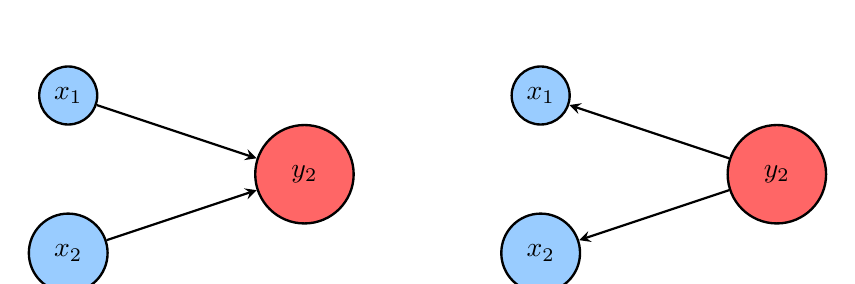
\begin{tikzpicture}


    % Define custom colors
    \definecolor{darkblue}{rgb}{0.6, 0.8, 1.0} % Defining dark blue
    \definecolor{darkred}{rgb}{1.0, 0.4, 0.4} % Defining dark red
    
 
    % Node styles
    \tikzset{every node/.style={circle, draw, line width=0.3mm}}
   
    
    % Nodes with different sizes and colors
    \node[fill=darkblue, minimum size=0.5cm] (x1) at (0-3,0) {$x_1$}; % Smaller node in dark blue
    \node[fill=darkblue, minimum size=1.0cm] (x2) at (0-3,-2) {$x_2$}; % Larger node in dark blue
    \node[fill=darkred, minimum size=1.25cm] (y2) at (3-3,-1) {$y_2$}; % Medium node in dark red
    
    % Arrows
    \draw[thick, ->, >=stealth] (x1) -- (y2);
    \draw[thick, ->, >=stealth] (x2) -- (y2);
    
    % Nodes with different sizes and colors
    \node[fill=darkblue, minimum size=0.5cm] (x1) at (0+3,0) {$x_1$}; % Smaller node in dark blue
    \node[fill=darkblue, minimum size=1.0cm] (x2) at (0+3,-2) {$x_2$}; % Larger node in dark blue
    \node[fill=darkred, minimum size=1.25cm] (y2) at (3+3,-1) {$y_2$}; % Medium node in dark red
    
    % Arrows
    \draw[thick, ->, >=stealth] (y2) -- (x1);
    \draw[thick, ->, >=stealth] (y2) -- (x2);    
    


\end{tikzpicture}

\caption{Schematic of discrete Monge OT. Let one define an optimal transport $T$ naturally as there is only one feasible transport map (Monge map). Right one does not have a compatible Monge map.} \label{fig:Monge_map} 


\end{figure}






\subsection[Discrete Kantorovich]{Kantorovich optimal transport for discrete measures}

As seen in the previous section, discrete Monge OT may not be well-defined in the absence of feasible solutions satisfying the mass conservation constraint (\ref{eqn:Monge_map_mass_conservation}). Additionally, discrete Monge OT is a nonconvex problem. Both drawbacks are therefore difficult to overcome.

The key idea of Kantorovich is to relax the deterministic nature of transportation, namely the fact that a source point \(x_i\) can only be assigned to another point or location \(y_{\sigma(i)}\), or \(T(x_i)\) only. Kantorovich proposes instead that the mass at any point \(x_i\) be potentially dispatched across several locations. Kantorovich moves away from the idea that mass transportation should be \textit{deterministic} to consider instead a \textit{probabilistic} transport, which allows what is commonly known now as \textit{mass splitting} from a source toward several targets. This flexibility is encoded using, in place of a permutation or a map \(T\), a coupling matrix \(\mathbf{P} = (P_{ij}) \in \mathbb{R}^{n \times m}\), where \(P_{ij}\) describes the amount of mass flowing from bin \(i\) to bin \(j\), or from the mass found at \(x_i\) toward \(y_j\) in the formalism of discrete measures (\ref{eqn:discrete_measure02}). Admissible couplings admit a far simpler characterization than Monge maps,
\begin{align}
\mathbf{U}(\mathbf{a}, \mathbf{b}) = \left\{ \mathbf{P} \in \mathbb{R}_+^{n \times m} : \mathbf{P}\mathbf{1} = \mathbf{a},  \mathbf{P}^{\text{T}}\mathbf{1} = \mathbf{b} \right\}, 
\end{align}
in which $\mathbf{1}$ represents all-one vector whose dimension is determined by dimension consistency of matrix multiplication in the context. In other words, the two constraints indicate that the row and column sums of $\mathbf{P}$ equal $\mathbf{a}$ and $\mathbf{b}$, respectively. The set of matrices \( \mathbf{U}(\mathbf{a}, \mathbf{b})  \) is bounded and defined by \( n+m \) equality constraints, and therefore is a convex polytope (the convex hull of a finite set of matrices).


\begin{figure}[t]
\center

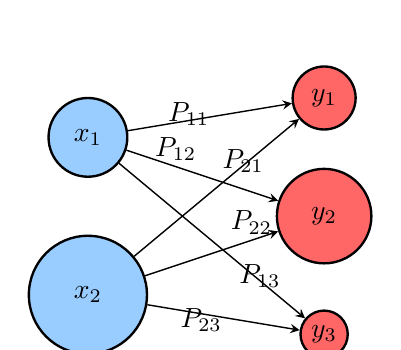
\begin{tikzpicture}

% Define custom colors
\definecolor{darkblue}{rgb}{0.6, 0.8, 1.0} % Defining dark blue
\definecolor{darkred}{rgb}{1.0, 0.4, 0.4} % Defining dark red

% Node styles
\tikzset{every node/.style={circle, draw, line width=0.3mm}}

\node[fill=darkblue, minimum size=1.0cm] (x1) at (0,1) {$x_1$}; 
\node[fill=darkblue, minimum size=1.5cm] (x2) at (0,-1) {$x_2$};
\node[fill=darkred, minimum size=0.8cm] (y1) at (3,1.5) {$y_1$};
\node[fill=darkred, minimum size=1.2cm] (y2) at (3,0) {$y_2$};
\node[fill=darkred, minimum size=0.6cm, inner sep=0] (y3) at (3,-1.5) {$y_3$};

% Arrows
\draw[line width = 0.5pt, ->, >=stealth] (x1) -- (y1) node[pos=0.6, left, fill=none, draw=none] {$P_{11}$};
\draw[line width = 0.5pt, ->, >=stealth] (x1) -- (y2) node[pos=0.5, above left, fill=none, draw=none] {$P_{12}$};
\draw[line width = 0.5pt, ->, >=stealth] (x1) -- (y3) node[pos=0.9, above left, fill=none, draw=none] {$P_{13}$};

\draw[line width = 0.5pt, ->, >=stealth] (x2) -- (y1) node[pos=0.5, above right, fill=none, draw=none] {$P_{21}$};
\draw[line width = 0.5pt, ->, >=stealth] (x2) -- (y2) node[pos=0.6,  above right, fill=none, draw=none] {$P_{22}$};
\draw[line width = 0.5pt, ->, >=stealth] (x2) -- (y3) node[pos=0.6, left, fill=none, draw=none] {$P_{23}$};

\end{tikzpicture}
\caption{Schematic of the coupling matrix $P$. \(P_{ij}\) describes the amount of mass flowing from bin \(i\) to bin \(j\), or from the mass found at \(x_i\) toward \(y_j\)} \label{fig:coupling_matrix} 

\end{figure}






\begin{definition}[Kantorovich OT between discrete measures]
Given discrete measures in (\ref{eqn:discrete_measure02})
and a cost function $c(x,y)$, Kantorovich OT between discrete measures is a minimization problem
\begin{align}
\mathcal{L}_{c}(\alpha, \beta) := \min_{\mathbf{P}\in \mathbf{U}(\mathbf{a}, \mathbf{b})} 
\sum_{i,j} P_{ij}c(x_i,y_j). \label{eqn:Kantorovich_discrete_01} 
\end{align}
If a cost matrix $\mathbf{C}$ is directly given, corresponding to the cost between $\{x_i\}_{i=1}^n$ and $\{y_j\}_{j=1}^m$, then the Kantorovich OT between probability vectors reads
\begin{align}
L_{\mathbf{C}}(\mathbf{a}, \mathbf{b}) := \min_{\mathbf{P}\in \mathbf{U}(\mathbf{a}, \mathbf{b})}  \langle \mathbf{P}, \mathbf{C} \rangle = 
\sum_{i,j} P_{ij} C_{ij}. \label{eqn:Kantorovich_discrete_02} 
\end{align}

\end{definition}


\begin{remark}
Discrete Kantorovich OT problem is a linear programming with convex constraints. Therefore the minimizers are achieved on the boundary of the convex polytope \( \mathbf{U}(\mathbf{a}, \mathbf{b})  \), and are not necessarily unique. See Figure \ref{fig:Linear_programming} for the schematic illustration.
\end{remark}

The Kantorovich problem (\ref{eqn:Kantorovich_discrete_02} ) is a constrained convex minimization problem, and as such, it can be naturally paired with a dual problem, which is a constrained concave maximization problem. The following fundamental proposition explains the relationship between the primal and dual problems.

\begin{proposition}[Discrete Kantorovich dual]
The Kantorovich problem (\ref{eqn:Kantorovich_discrete_02}) admits the dual
\begin{align}
L_{\mathbf{C}}(\mathbf{a}, \mathbf{b}) = \max_{(\mathbf{f}, \mathbf{g}) \in \mathbf{R}(\mathbf{C})} \langle \mathbf{f}, \mathbf{a} \rangle + \langle \mathbf{g}, \mathbf{b} \rangle,
\end{align}
where the set of feasible dual variables is
\begin{align}
\mathbf{R}(\mathbf{C}) := \{(\mathbf{f}, \mathbf{g}) \in \mathbb{R}^n \times \mathbb{R}^m : \forall (i, j) \in [n] \times [m], \mathbf{f} \oplus \mathbf{g} \leq \mathbf{C} \}. 
\end{align}
Such dual variables are often referred to as ``Kantorovich potentials''.
\end{proposition}


\begin{figure}[t]
\center
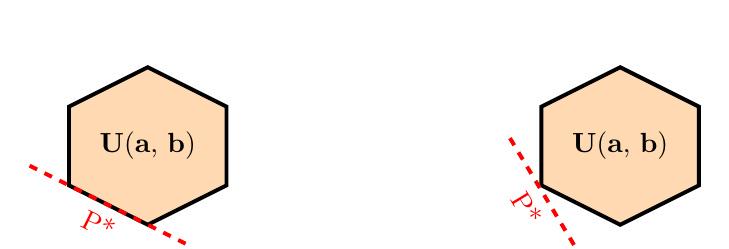
\begin{tikzpicture}

    % Define the hexagon
    \draw[fill=orange!30, line width=0.5mm] (0-3,0) -- (1-3,0.5) -- (1-3,1.5) -- (0-3,2) -- (-1-3,1.5) -- (-1-3,0.5) -- cycle;
    % Label the polygon
    \node at (0-3,1) {\textbf{U}(\textbf{a}, \textbf{b})};

    % Define and label the dashed line
    \draw[dashed, red, thick, line width=0.5mm] (-1.5-3,0.75) -- (0.5-3,-0.25) node[midway, below, sloped] {P*};

     % Define the hexagon
    \draw[fill=orange!30, line width=0.5mm] (0+3,0) -- (1+3,0.5) -- (1+3,1.5) -- (0+3,2) -- (-1+3,1.5) -- (-1+3,0.5) -- cycle;
    % Label the polygon
    \node at (0+3,1) {\textbf{U}(\textbf{a}, \textbf{b})};

    % Define and label the dashed line
    \draw[dashed, red, thick, line width=0.5mm] (-1.4+3,1.1) -- (-0.5+3,-0.4) node[midway, below, sloped] {P*};

\end{tikzpicture}

\caption{Schematic of optimal solutions of linear programming. Left: optimal solutions are not unique; Right: optimal solution is unique.} \label{fig:Linear_programming} 

\end{figure}




\section[Wasserstein Distance]{Wasserstein Distance and Metric Property}


Let $(X,d)$ be a locally compact and separable metric space. A model case is $(X,d) = (\mathbb{R}^n, \|x-y\|_2)$. Now we define the $p$-Wasserstein distance as follows:
\begin{definition}[$p$-Wasserstein distance]
Given \(\mu, \nu \in \mathcal{P}(X)\), we define their \(p\)-Wasserstein distance as
\begin{align}
W_p(\mu, \nu) := \left( \inf_{\gamma \in \Gamma(\mu, \nu)} \int_{X \times X} d(x, y)^p \, d\gamma(x, y) \right)^{\frac{1}{p}}.
\end{align}
\end{definition}

\begin{theorem}[Metric property]
$W_p$ is a distance on the space $\mathcal{P}(X)$, namely, $W_p$ is symmetric, nonnegative, $W_p(\mu,\nu) = 0$ if and only if $\mu = \nu$, and it satisfies the triangle inequality:
\begin{align*}
W_p(\mu,\nu) \le W_p(\mu,\sigma) + W_p(\sigma,\nu), \quad \forall \mu,\nu,\sigma \in \mathcal{P}(X).
\end{align*}
\end{theorem}

Define the discrete $p$-Wasserstein distance as
\begin{align}
W_p(\mathbf{a},\mathbf{b}) : = \left(\min_{\mathbf{P}\in \mathbf{U}(\mathbf{a}, \mathbf{b})}  \langle \mathbf{P}, \mathbf{D}^p \rangle \right)^{\frac{1}{p}} = \Big( L_{\mathbf{D}^p}(\mathbf{a},\mathbf{b}) \Big)^{\frac{1}{p}},
\end{align}
where $\mathbf{D} \in \mathbb{R}_+^{n\times n}$ is a distance on $[n]$, namely,
\begin{itemize}
    \item[(i)] \(\mathbf{D} \in \mathbb{R}^{n \times n}_+\) is symmetric;
    \item[(ii)] \(D_{ij} = 0\) if and only if \(i = j\);
    \item[(iii)] \(D_{ik} \leq D_{ij} + D_{jk}\), for $\forall (i, j, k) \in [n]^3$.
\end{itemize}
Then the $p$-Wasserstein distsnce $W_p(\mathbf{a},\mathbf{b})$ is a distance on probability simplex $\Sigma_n$.


























\chapter[Entropic Regularization]{Entropic Regularization of Optimal Transport}

Note that Kantorovich OT (\ref{eqn:Kantorovich_discrete_02}) is a linear programming with convex constraints, therefore simplex algorithm or interior point methods can be naturally adopted. However, the computational cost for these methods are $O(N^3 \log N), N = \max\{n,m\}$, hence inefficient. 

This chapter introduces a family of numerical schemes to approximate solutions to Kantorovich formulation of optimal transport (\ref{eqn:Kantorovich_discrete_02}) and its many generalizations. It operates by adding an entropic regularization penalty to the original problem. This regularization has several important advantages, which make it, when taken altogether, a very useful tool: the minimization of the regularized problem can be solved using a simple alternate minimization scheme; that scheme translates into iterations that are simple matrix-vector products, making them particularly suited to execution on GPU; for some applications, these matrix-vector products do not require storing an \(n \times m\) cost matrix, but instead only require access to a kernel evaluation; in the case where a large group of measures share the same support, all of these matrix-vector products can be cast as matrix-matrix products with significant speedups; the resulting approximate distance is smooth with respect to input histogram weights and positions of the Diracs and can be differentiated using automatic differentiation.


\section[Entropic Regularization]{Entropic Regularization}

The discrete entropy of a coupling matrix is defined as
\begin{equation}
H(\mathbf{P}) := -\sum_{i,j} P_{ij} \log(P_{ij} - 1), 
\end{equation}
with an analogous definition for vectors, with the convention that \(\mathbf{H}(\mathbf{a}) = -\infty\) if one of the entries is \(0\) or negative. The function \(H\) is \(1\)-strongly concave, because its Hessian is \(\nabla^2 H(P) = -\text{diag}(1/P_{ij})\) and \(P_{ij} \leq 1\). The idea of the entropic regularization of optimal transport is to use \(-H\) as a regularizing function to obtain approximate solutions to the original transport problem (\ref{eqn:Kantorovich_discrete_02}).

\begin{definition}
The entropic regularization of the Kantorovich OT is defined as
\begin{align}\label{eqn:OT_entropic}
L_{\mathbf{C}}^{\epsilon}(\mathbf{a}, \mathbf{b}) = W_{\epsilon}(\mathbf{a}, \mathbf{b}) = \min_{\mathbf{P} \in \mathbf{U}(\mathbf{a},\mathbf{b})} \langle \mathbf{P}, \mathbf{C} \rangle - \epsilon H(\mathbf{P}).
\end{align}
\end{definition}
Here we use two notations for the entropic approximation. The two notations $L_{\mathbf{C}}^{\epsilon}(\mathbf{a}, \mathbf{b})$ and $W_{\epsilon}(\mathbf{a}, \mathbf{b})$ will be used interchangeably hereafter.

Since the objective is an \(\epsilon\)-strongly convex function, Problem (\ref{eqn:OT_entropic}) has a unique optimal solution. The idea to regularize the optimal transport problem by an entropic term can be traced back to modeling ideas in transportation theory: Actual traffic patterns in a network do not agree with those predicted by the solution of the optimal transport problem. Indeed, the former are more diffuse than the latter, which tend to rely on a few routes as a result of the sparsity of optimal couplings for. To mitigate this sparsity, researchers in transportation proposed a model, called the ``gravity'' model, that is able to form a more ``blurred'' prediction of traffic given marginals and transportation costs.

\begin{proposition}[Convergence with \(\epsilon\)]
The unique solution \(\mathbf{P}_{\epsilon}^*\) of (\ref{eqn:OT_entropic}) converges to the optimal solution with maximal entropy within the set of all optimal solutions of the Kantorovich problem, namely
\begin{equation}
\lim_{\epsilon \to 0}\mathbf{P}^*_{\epsilon}  = \underset{ \mathbf{P}}{\mathrm{argmin}}  \left\{-H(\mathbf{P}) : \mathbf{P} \in \mathbf{U}(\mathbf{a},\mathbf{b}), \ \ \langle \mathbf{P}, \mathbf{C} \rangle = L_{\mathbf{C}}(\mathbf{a}, \mathbf{b})\right\},
\end{equation}
so that in particular
\begin{equation}
\lim_{\epsilon \to 0} L_{C}^{\epsilon}(\mathbf{a}, \mathbf{b}) = L_{\mathbf{C}}(\mathbf{a}, \mathbf{b}). 
\end{equation}
One also has
\begin{equation}
\lim_{\epsilon \to \infty}\mathbf{P}^*_{\epsilon} = \mathbf{a} \otimes \mathbf{b} = \mathbf{a}\mathbf{b}^{\emph{T}} = (a_i b_j)_{i,j}. 
\end{equation}
\end{proposition}

Defining the Kullback--Leibler divergence between couplings as
\begin{equation}
\text{KL}(\mathbf{P}|\mathbf{K}) = \sum_{i,j} P_{ij} \log \left(\frac{P_{ij}}{K_{ij}}\right) -P_{ij} + K_{ij}, \tag{4.6}
\end{equation}
the unique solution \(\mathbf{P}^*_{\epsilon}\) of (\ref{eqn:OT_entropic}) is a projection onto \(\mathbf{U}(\mathbf{a}, \mathbf{b})\) of the Gibbs kernel associated to the cost matrix \(\mathbf{C}\) as
\[
\mathbf{K} := e^{-\frac{\mathbf{C}}{\epsilon}}.
\]
Indeed one has that using the definition above that
\begin{equation}\label{eqn:KL_proj}
\mathbf{P}^*_{\epsilon} = \text{Proj}_{\mathbf{U}(\mathbf{a},\mathbf{b})}^{\text{KL}}(\mathbf{K}) := \underset{ \mathbf{P} \in \mathbf{U}(\mathbf{a},\mathbf{b})}{\mathrm{argmin}} \text{KL}(\mathbf{P} | \mathbf{K}).
\end{equation}
In other words, the unique solution of the entropic OT is the projection of $\mathbf{K}$ onto $\mathbf{U}(\mathbf{a},\mathbf{b})$ with respect to KL divergence.

\begin{definition}[Entropic regularization between discrete measures]
For discrete measures of the form (\ref{eqn:discrete_measure02}), the definition of regularized optimal transport extends naturally to
\begin{equation}
\mathcal{L}_{c}^{\epsilon}(\alpha, \beta) := L_{\mathbf{C}}^{\epsilon}(a, b),
\end{equation}
with cost \( C_{ij} = c(x_i, y_j) \), to emphasize the dependency with respect to the positions \( (x_i, y_j) \) supporting the input measures.
\end{definition}






\section[Sinkhorn]{Sinkhorn's Algorithm}


In this section, we introduce the Sinkhorn algorithm, a major breakthrough of the past decade \cite{cuturi2013sinkhorn}, which has revitalized the application of optimal transport across diverse fields. We begin by presenting the following lemma, which indicates that the solution to the entropic regularized OT problem has a so-called {\it diagonal rescaling decomposition}.


\begin{proposition}[Diagonal rescaling decomposition]\label{proposition:diagonal_rescaling}
The solution to (\ref{eqn:OT_entropic}) is unique and has the form $\mathbf{P} = \mathrm{diag}(\mathbf{u})\mathbf{K}\mathrm{diag}(\mathbf{v})$, or componentwisely
\begin{align*}
P_{i,j} = u_i K_{i,j} v_j,    \quad  \forall (i,j) \in [n] \times [m]
\end{align*}
for two (unknown) scaling variables $(\mathbf{u}, \mathbf{v}) \in \mathbb{R}_+^n \times \mathbb{R}_+^m$.
\end{proposition}

\begin{proof}
Introducing two dual variables $\mathbf{f} \in \mathbb{R}^n, \mathbf{g} \in \mathbb{R}^m$ for each marginal constraint, the Lagrangian of \eqref{eqn:OT_entropic} reads
\begin{align*}
    \mathcal{L}(\mathbf{P}; \mathbf{f}, \mathbf{g}) = \langle \mathbf{P}, \mathbf{C} \rangle - \epsilon H(\mathbf{P}) - \langle \mathbf{f}, \mathbf{P} \mathbb{1} - \mathbf{a} \rangle - \langle \mathbf{g}, \mathbf{P}^{\mathrm{T}} \mathbb{1} - \mathbf{b} \rangle.
\end{align*}

First-order conditions then yield
\begin{align*}
    \frac{\partial \mathcal{L}(\mathbf{P}, \mathbf{f}, \mathbf{g})}{\partial P_{i,j}} = C_{i,j} + \epsilon \log (P_{i,j}) - f_i - g_j = 0,
\end{align*}
from which we get
\begin{align*}
    P_{i,j} = e^{f_i/\epsilon} e^{-C_{i,j}/\epsilon} e^{g_j/\epsilon},
\end{align*}
or in the matrix form
\begin{align*}
    \mathbf{P} = \text{diag}(e^{\mathbf{f}/\epsilon}) e^{-\mathbf{C}/\epsilon} \text{diag}(e^{\mathbf{g}/\epsilon}).
\end{align*}
Taking $\mathbf{u} = e^{\mathbf{f}/\epsilon}, \mathbf{v} = e^{\mathbf{g}/\epsilon}, \mathbf{K} = e^{-\mathbf{C}/\epsilon}$, the diagonal rescaling decomposition is obtained.
\end{proof}

The above proposition implies that the unknown variables $(\mathbf{u},\mathbf{v})$ satisfy the following nonlinear equations which corresond to the mass conservation constraints $\mathbf{P} \in \mathbf{U}(\mathbf{a},\mathbf{b})$:
\begin{align*}
    \operatorname{diag}(\mathbf{u}) \mathbf{K} \operatorname{diag}(\mathbf{v}) \mathbb{1} &= \mathbf{a}, 
    \quad \operatorname{diag}(\mathbf{v}) \mathbf{K}^{\mathrm{T}} \operatorname{diag}(\mathbf{u}) \mathbb{1} = \mathbf{b}.
\end{align*}
These two equations can be further simplified, since $\operatorname{diag}(\mathbf{v}) \mathbb{1}$ is simply $\mathbf{v}$, and the multiplication of $\operatorname{diag}(\mathbf{u})$ times $\mathbf{K} \mathbf{v}$ is  
\begin{align}\label{eqn:Sinkhorn00}
    \mathbf{u} \odot (\mathbf{K} \mathbf{v}) = \mathbf{a},  
    \quad \mathbf{v} \odot (\mathbf{K}^{\mathrm{T}} \mathbf{u}) = \mathbf{b},
\end{align}
where $\odot$ corresponds to entrywise multiplication of vectors. That problem is known in the numerical analysis community as the matrix scaling problem. An intuitive way to handle these equations is to solve them iteratively, by modifying first $\mathbf{u}$ so that it satisfies the left-hand side of Equation \eqref{eqn:Sinkhorn00}, and then $\mathbf{v}$ to satisfy its right-hand side. These two updates define {\it Sinkhorn’s algorithm},

\begin{align}\label{eqn:Sinkhorn01}
    \mathbf{u}^{(\ell+1)} := \frac{\mathbf{a}}{\mathbf{K} \mathbf{v}^{(\ell)}},  
    \quad \mathbf{v}^{(\ell+1)} &:= \frac{\mathbf{b}}{\mathbf{K}^{\mathrm{T}} \mathbf{u}^{(\ell+1)}}, 
\end{align}
initialized with an arbitrary positive vector $\mathbf{v}^{(0)} = \mathbb{1}$. The division operator used above between two vectors is to be understood entrywise. 

Note that a different initialization will likely lead to a different solution for $\mathbf{u}, \mathbf{v}$, since $\mathbf{u}, \mathbf{v}$ are only defined up to a multiplicative constant (if $\mathbf{u}, \mathbf{v}$ satisfy \eqref{eqn:Sinkhorn00}, then so do $\lambda \mathbf{u}, \mathbf{v}/\lambda$ for any $\lambda > 0$). It turns out, however, that these iterations converge and all result in the same optimal coupling $\operatorname{diag}(\mathbf{u}) \mathbf{K} \operatorname{diag}(\mathbf{v})$, which is evolved from the Gibbs kernel $\mathbf{K}$ by progressively shifting the mass away from the diagonal.

\begin{remark}[Overall complexity]
By performing a careful convergence analysis (assuming $n = m$ for simplicity), \cite{altschuler2017near} showed that by setting $\epsilon = \frac{4 \log(n)}{\tau}$, $O(\|\mathbf{C}\|_{\infty}^3 \log(n) \tau^{-3})$ Sinkhorn iterations (with an additional rounding step to compute a valid coupling $\hat{\mathbf{P}} \in \mathbf{U}(\mathbf{a}, \mathbf{b})$) are sufficient to ensure that
\begin{align*}
    \langle \hat{\mathbf{P}}, \mathbf{C} \rangle \leq L_{\mathbf{C}}(\mathbf{a}, \mathbf{b}) + \tau.
\end{align*}
This implies that Sinkhorn computes a $\tau$-approximate solution of the unregularized OT problem in $O(n^2 \log(n) \tau^{-3})$ operations. 
\end{remark}

Note that Sinkhorn algorithm \eqref{eqn:Sinkhorn01} is equivalent to the Bregman iteration. We summarize it in the following lemma.
\begin{lemma}[Bregman interation]
Denoting
\begin{align*}
    \mathcal{C}_\mathbf{a} \coloneqq \{\mathbf{P} : \mathbf{P} \mathbb{1} = \mathbf{a} \},  
    \quad \mathcal{C}_\mathbf{b} \coloneqq \{\mathbf{P} : \mathbf{P}^\mathrm{T} \mathbb{1} = \mathbf{b} \}
\end{align*}
as the row and column constraints, we have $\mathbf{U}(\mathbf{a}, \mathbf{b}) = \mathcal{C}_\mathbf{a} \cap \mathcal{C}_\mathbf{b}$. One can use Bregman iterative projections \cite{bregman1967relaxation},  
\begin{align}\label{eqn:Bregman}
    \mathbf{P}^{(\ell+1)} \coloneqq \operatorname{Proj}^{\operatorname{KL}}_{\mathcal{C}_\mathbf{a}} (\mathbf{P}^{(\ell)})  
    & \quad  
    \mathbf{P}^{(\ell+2)} \coloneqq \operatorname{Proj}^{\operatorname{KL}}_{\mathcal{C}_\mathbf{b}} (\mathbf{P}^{(\ell+1)}).
\end{align}
Since the sets $\mathcal{C}_\mathbf{a}$ and $\mathcal{C}_\mathbf{b}$ are affine, these iterations are known to converge to the solution of \eqref{eqn:KL_proj}; see \cite{bregman1967relaxation}. These iterates are equivalent to Sinkhorn iterations \eqref{eqn:Sinkhorn01}.
\end{lemma}

\begin{proof}
We only prove the equivalence between Sinkhorn and Bregman. The convergence can be found in the reference. Assuming we have a diagonally rescaling decomposition at $(2\ell)$-th step: 
\begin{align*}
    \mathbf{P}^{(2\ell)} &\coloneqq \operatorname{diag}(\mathbf{u}^{(\ell)}) \mathbf{K} \operatorname{diag}(\mathbf{v}^{(\ell)}).
\end{align*}
Now let us consider the KL projection problem in \eqref{eqn:Bregman}:
\begin{align*}
    \mathbf{P}^{(2\ell+1)} = \operatorname{Proj}^{\operatorname{KL}}_{\mathcal{C}_\mathbf{a}} (\mathbf{P}^{(2\ell)}) = \operatorname{argmin}_{\mathbf{P}\in\mathcal{C}_{\mathbf{a}}} \epsilon\operatorname{KL}(\mathbf{P}|\mathbf{P}^{2\ell}).
\end{align*}
Rewrite this constrained problem in Lagrangian form
\begin{align*}
    \mathcal{L}(\mathbf{P};\mathbf{f}) = \epsilon\operatorname{KL}(\mathbf{P}|\mathbf{P}^{2\ell}) - \langle \mathbf{f}, \mathbf{P} \mathbb{1} - \mathbf{a} \rangle
\end{align*}
and take the first-order derivative, we have
\begin{align*}
    \frac{\partial \mathcal{L}(\mathbf{P};\mathbf{f})}{\partial P_{i,j}} =  \epsilon \log \frac{P_{ij}}{P_{ij}^{(2\ell)}} - f_i = 0 
     \Rightarrow  P_{ij} = e^{f_i/\epsilon}P_{ij}^{(2\ell)} 
     \Rightarrow \mathbf{P}^{(2\ell+1)} = \operatorname{diag}(e^{\mathbf{f}/\epsilon})\mathbf{P}^{(2\ell)}.
\end{align*}
From the constraint of $\mathcal{C}_\mathbf{a}$, 
\begin{align*}
    \mathbf{P}^{(2\ell+1)}\mathbb{1}= \mathbf{a} \Rightarrow \operatorname{diag}(e^{\mathbf{f}/\epsilon})\mathbf{P}^{(2\ell)}\mathbb{1} = e^{\mathbf{f}/\epsilon}\odot(\mathbf{P}^{(2\ell)}\mathbb{1}) = \mathbf{a} \Rightarrow 
    e^{\mathbf{f}/\epsilon} = \frac{\mathbf{a}}{\mathbf{P}^{(2\ell)}\mathbb{1}}.
\end{align*}
Then 
\begin{align*}
    \mathbf{P}^{(2\ell+1)} & = \operatorname{diag}(e^{\mathbf{f}/\epsilon})\mathbf{P}^{(2\ell)} \\
    & = \operatorname{diag}\left(\frac{\mathbf{a}}{\mathbf{P}^{(2\ell)}\mathbb{1}}\right)\mathbf{P}^{(2\ell)} \\
    & = \operatorname{diag}\left(\frac{\mathbf{a}}{ \mathbf{u}^{(\ell)} \odot (\mathbf{K} \mathbf{v}^{(\ell)})  }\right) \operatorname{diag}(\mathbf{u}^{(\ell)}) \mathbf{K} \operatorname{diag}(\mathbf{v}^{(\ell)}) \\
    & = \operatorname{diag}\left(\frac{\mathbf{a}}{ \mathbf{K} \mathbf{v}^{(\ell)}  }\right) \mathbf{K} \operatorname{diag}(\mathbf{v}^{(\ell)})
\end{align*}
from which we see that the update from $\mathbf{P}^{(2\ell)} \rightarrow \mathbf{P}^{(2\ell+1)}$ is equivalent to take $\mathbf{u}^{(\ell)} \rightarrow \frac{\mathbf{a}}{ \mathbf{K} \mathbf{v}^{(\ell)} }: = \mathbf{u}^{(\ell+1)}$:
\begin{align*}
    \mathbf{P}^{(2\ell+1)} &\coloneqq \operatorname{diag}(\mathbf{u}^{(\ell+1)}) \mathbf{K} \operatorname{diag}(\mathbf{v}^{(\ell)}).
\end{align*}
Similarly the update from $\mathbf{P}^{(2\ell+1)} \rightarrow \mathbf{P}^{(2\ell+2)}$ is equivalent to take $\mathbf{v}^{(\ell)} \rightarrow \frac{\mathbf{b}}{ \mathbf{K}^{\mathrm{T}} \mathbf{u}^{(\ell+1)} }: = \mathbf{v}^{(\ell+1)}$:
\begin{align*}
    \mathbf{P}^{(2\ell+2)} &\coloneqq \operatorname{diag}(\mathbf{u}^{(\ell+1)}) \mathbf{K} \operatorname{diag}(\mathbf{v}^{(\ell+1)}).
\end{align*}
The equivalence is proved.
\end{proof}








\section[Sinkhorn in Log-Domain]{Sinkhorn's Algorithm in Log Domain}


The convergence of Sinkhorn's algorithm deteriorates as $\epsilon \to 0$. In numerical practice, however, that slowdown is rarely observed for a simpler reason: Sinkhorn's algorithm will often fail to terminate as soon as some of the elements of the kernel $\mathbf{K}$ become too negligible to be stored in memory as positive numbers and instead become null. This can result in a matrix product $\mathbf{K} \mathbf{v}$ or $\mathbf{K}^\mathrm{T} \mathbf{u}$ with increasingly smaller entries that eventually become null, leading to a division by $0$ in the Sinkhorn update of Equation \eqref{eqn:Sinkhorn01}. Such issues can be partly resolved by carrying out computations on the multipliers $\mathbf{u}$ and $\mathbf{v}$ in the log domain. The relevance of this approach is made more clear by considering the dual problem associated to \eqref{eqn:OT_entropic}, in which the log-domain computations arise naturally.
    
\begin{proposition}[Dual form of entropic OT]
    The primal entropic regularized OT \eqref{eqn:OT_entropic} admits a dual form
    \begin{align}\label{eqn:OT_entropic_dual}
        L_\mathbf{C}^\epsilon (\mathbf{a}, \mathbf{b}) = \max_{\mathbf{f} \in \mathbb{R}^n, \mathbf{g} \in \mathbb{R}^m} \langle \mathbf{f}, \mathbf{a} \rangle + \langle \mathbf{g}, \mathbf{b} \rangle - \epsilon \langle e^{\mathbf{f} / \epsilon}, \mathbf{K} e^{\mathbf{g} / \epsilon} \rangle.
    \end{align}
    
    The optimal $(\mathbf{f}, \mathbf{g})$ are linked to the scalings $(\mathbf{u}, \mathbf{v})$ appearing in Sinkhorn through
    \begin{align}\label{eqn:primal_dual_variables}
        (\mathbf{u}, \mathbf{v}) = (e^{\mathbf{f} / \epsilon}, e^{\mathbf{g} / \epsilon}).
    \end{align}
\end{proposition}
    
\begin{proof}
    We start from the end of the proof of Proposition \ref{proposition:diagonal_rescaling}, which links the optimal primal solution $\mathbf{P}$ and dual multipliers $\mathbf{f}$ and $\mathbf{g}$ for the marginal constraints as
    \begin{align*}
        P_{i,j} = e^{f_i / \epsilon} e^{-C_{i,j} / \epsilon} e^{g_j / \epsilon} \Leftrightarrow \mathbf{P} = e^{\frac{-\mathbf{C}+\mathbf{f}\oplus\mathbf{g}}{\epsilon}}.
    \end{align*}
    Substituting into the Lagrangian $\mathcal{L}(\mathbf{P}, \mathbf{f}, \mathbf{g})$ of Equation \eqref{eqn:OT_entropic}, we have
    \begin{align*}
        \mathcal{L}(\mathbf{P};\mathbf{f},\mathbf{g}) & = \langle \mathbf{P}, \mathbf{C}  \rangle + \epsilon \left\langle \mathbf{P}, \frac{-\mathbf{C}+\mathbf{f}\oplus\mathbf{g}}{\epsilon} - \mathbb{1}  \right\rangle  - \langle \mathbf{f}, \mathbf{P} \mathbb{1} - \mathbf{a} \rangle - \langle \mathbf{g}, \mathbf{P}^{\mathrm{T}} \mathbb{1} - \mathbf{b} \rangle \\
        & = \langle \mathbf{P}, \mathbf{C}  \rangle + \left\langle \mathbf{P}, -\mathbf{C}+\mathbf{f}\oplus\mathbf{g} - \epsilon\mathbb{1}  \right\rangle  - \langle \mathbf{f}, \mathbf{P} \mathbb{1} - \mathbf{a} \rangle - \langle \mathbf{g}, \mathbf{P}^{\mathrm{T}} \mathbb{1} - \mathbf{b} \rangle \\
        & = \left\langle \mathbf{P}, \mathbf{f}\mathbb{1}^{\mathrm{T}}+\mathbb{1}\mathbf{g}^{\mathrm{T}} - \epsilon\mathbb{1}  \right\rangle - \langle \mathbf{f}, \mathbf{P} \mathbb{1} - \mathbf{a} \rangle - \langle \mathbf{g}, \mathbf{P}^{\mathrm{T}} \mathbb{1} - \mathbf{b} \rangle \\
        & = \langle \mathbf{f}, \mathbf{P}\mathbb{1} \rangle + \langle \mathbf{g}, \mathbf{P}^{\mathrm{T}}\mathbb{1} \rangle - \epsilon \langle \mathbf{P}, \mathbb{1} \rangle - \langle \mathbf{f}, \mathbf{P} \mathbb{1} - \mathbf{a} \rangle - \langle \mathbf{g}, \mathbf{P}^{\mathrm{T}} \mathbb{1} - \mathbf{b} \rangle \\
        & = \langle \mathbf{f}, \mathbf{a} \rangle + \langle \mathbf{g}, \mathbf{b} \rangle - \epsilon \langle \mathbf{P}, \mathbb{1} \rangle  \\
        & = \langle \mathbf{f}, \mathbf{a} \rangle + \langle \mathbf{g}, \mathbf{b} \rangle - \epsilon \langle e^{\mathbf{f}/\epsilon}, \mathbf{K}e^{\mathbf{g}/\epsilon} \rangle
    \end{align*}
    Then take maximum over $(\mathbf{f},\mathbf{g})$ for $\mathcal{L}(\mathbf{P};\mathbf{f},\mathbf{g})$, we obtain the dual form as required.

    Besides, by the argument of strong duality, the primal and the dual form are equivalent.
\end{proof}
    
\begin{proposition}[Sinkhorn as a block coordinate ascent on the dual problem]
    A straightforward approach to solving the unconstrained maximization problem \eqref{eqn:OT_entropic_dual} is to use an exact block coordinate ascent strategy, namely to update alternatively $\mathbf{f}$ and $\mathbf{g}$ to cancel the respective gradients in these variables of the objective of \eqref{eqn:OT_entropic_dual}:
    \begin{align*}
        \mathbf{f}^{(\ell+1)} &= \varepsilon \log \mathbf{a} - \varepsilon \log \left( \mathbf{K} e^{\mathbf{g}^{(\ell)} / \varepsilon} \right), \\
        \mathbf{g}^{(\ell+1)} &= \varepsilon \log \mathbf{b} - \varepsilon \log \left( \mathbf{K}^{\mathrm{T}} e^{\mathbf{f}^{(\ell+1)} / \varepsilon} \right),
    \end{align*}
    which is equivalent to the Sinkhorn algorithm.
\end{proposition}

\begin{proof}
    Let $Q(\mathbf{f}, \mathbf{g})$ be the objective of \eqref{eqn:OT_entropic_dual}, then the derivatives of $Q$ with respect to $\mathbf{f}$ and $\mathbf{g}$ are:
    \begin{align*}
        \nabla_{\mathbf{f}} Q(\mathbf{f}, \mathbf{g}) &= \mathbf{a} - e^{\mathbf{f} / \varepsilon} \odot (\mathbf{K} e^{\mathbf{g} / \varepsilon}), \\
        \nabla_{\mathbf{g}} Q(\mathbf{f}, \mathbf{g}) &= \mathbf{b} - e^{\mathbf{g} / \varepsilon} \odot (\mathbf{K}^{\mathrm{T}} e^{\mathbf{f} / \varepsilon}).
    \end{align*}
    Block coordinate ascent can therefore be implemented in a closed form by applying 
    successively the following updates, starting from any arbitrary $\mathbf{g}^{(0)}$, for $l \geq 0$:
    \begin{align*}
        &\nabla_{\mathbf{f}} Q(\mathbf{f}^{(\ell+1)}, \mathbf{g}^{(\ell)}) = 0 \quad \Rightarrow \mathbf{f}^{(\ell+1)} = \varepsilon \log \mathbf{a} - \varepsilon \log \left( \mathbf{K} e^{\mathbf{g}^{(\ell)} / \varepsilon} \right),\\
        &\nabla_{\mathbf{g}} Q(\mathbf{f}^{(\ell+1)}, \mathbf{g}^{(\ell+1)}) = 0 \Rightarrow  \mathbf{g}^{(\ell+1)} = \varepsilon \log \mathbf{b} - \varepsilon \log \left( \mathbf{K}^{\mathrm{T}} e^{\mathbf{f}^{(\ell+1)} / \varepsilon} \right),
    \end{align*}
    Such iterations are mathematically equivalent to the Sinkhorn iterations \eqref{eqn:Sinkhorn01} when considering the primal-dual relations highlighted in \eqref{eqn:primal_dual_variables}. Indeed, we recover that at any iteration
    \begin{align*}
        (\mathbf{f}^{(\ell)}, \mathbf{g}^{(\ell)}) = \varepsilon (\log (\mathbf{u}^{(\ell)}), \log (\mathbf{v}^{(\ell)})).
    \end{align*}
    Proof is completed.
\end{proof}

The Sinkhorn iteration in log-domain can be rewritten using soft-min. Given $\mathbf{z} = \{z_i\}_{i=1}^n$, $\min_i z_i$ can be approximated by using log-sum-exp function:
\begin{align*}
    \min_{\epsilon} \mathbf{z} = -\epsilon \log \left( \sum_i \exp\left(-\frac{z_i}{\epsilon}\right) \right).
\end{align*}
This approximation is due to the following lemmas.
\begin{lemma}
    Define soft-max function (log-sum-exp (LSE))
    \begin{align*}
        \operatorname{LSE}(x_1,\cdots,x_n) = \log(e^{x_1}+\cdots+e^{x_n}),
    \end{align*}
    then $\operatorname{LSE}$ is an approximation of the standard $\max$ in the sense that
    \begin{align*}
        \max\{x_1,\cdots,x_n\} \le \operatorname{LSE}(x_1,\cdots,x_n) \le \max\{x_1,\cdots,x_n\}+\log n.
    \end{align*}
\end{lemma}
\begin{proof}
    Obviously
    \begin{align*}
        e^{x_{\max}}\le \sum_i e^{x_i} \le \sum_i e^{x_{\max}}=n e^{x_{\max}}.
    \end{align*}
    Take $\log$ on both sides, we have the two inequalities.
\end{proof}
\begin{lemma}
    There is a tighter bound below
    \begin{align*}
        \max\{x_1,\cdots,x_n\} \le \epsilon \operatorname{LSE}\left(\frac{x_1}{\epsilon},\cdots,\frac{x_n}{\epsilon}\right) \le \max\{x_1,\cdots,x_n\}+\epsilon\log n.
    \end{align*}
\end{lemma}
\begin{lemma}
    The soft-min has an estimate
    \begin{align*}
        \min\{x_1,\cdots,x_n\} - \epsilon\log n \le - \epsilon \operatorname{LSE}\left(-\frac{x_1}{\epsilon},\cdots,-\frac{x_n}{\epsilon}\right) \le \min\{x_1,\cdots,x_n\}.
    \end{align*}
\end{lemma}
\begin{proof}
    It is obvious from the tighter bound that
    \begin{align*}
       &\max\left\{\frac{x_1}{\epsilon},\cdots,\frac{x_n}{\epsilon}\right\} \le  \operatorname{LSE}\left(\frac{x_1}{\epsilon},\cdots,\frac{x_n}{\epsilon}\right) \le \max\left\{\frac{x_1}{\epsilon},\cdots,\frac{x_n}{\epsilon}\right\}+\log n \\
       \Rightarrow &\max\left\{-\frac{x_1}{\epsilon},\cdots,-\frac{x_n}{\epsilon}\right\} \le  \operatorname{LSE}\left(-\frac{x_1}{\epsilon},\cdots,-\frac{x_n}{\epsilon}\right) \le \max\left\{-\frac{x_1}{\epsilon},\cdots,-\frac{x_n}{\epsilon}\right\}+\log n \\
       \Rightarrow &-\max\left\{-\frac{x_1}{\epsilon},\cdots,-\frac{x_n}{\epsilon}\right\} \ge  -\operatorname{LSE}\left(-\frac{x_1}{\epsilon},\cdots,-\frac{x_n}{\epsilon}\right) \ge -\max\left\{-\frac{x_1}{\epsilon},\cdots,-\frac{x_n}{\epsilon}\right\}-\log n \\      
       \Rightarrow &\min\left\{\frac{x_1}{\epsilon},\cdots,\frac{x_n}{\epsilon}\right\} \ge  -\operatorname{LSE}\left(-\frac{x_1}{\epsilon},\cdots,-\frac{x_n}{\epsilon}\right) \ge \min\left\{\frac{x_1}{\epsilon},\cdots,\frac{x_n}{\epsilon}\right\}-\log n
    \end{align*}
    multiplying $\epsilon$ on two sides, the estimate is obtained.
\end{proof}
Now for the term $-\epsilon \log(\mathbf{K}e^{\mathbf{g}^{(\ell)}/\epsilon})$, we have
\begin{align*}
    -\epsilon \log(\mathbf{K}e^{\mathbf{g}^{(\ell)}/\epsilon}) = 
    -\epsilon \log
    \begin{pmatrix*}[r]
        \exp(-\frac{C_{11}-g_1^{(\ell)}}{\epsilon}) + \cdots + \exp(-\frac{C_{1m}-g_m^{(\ell)}}{\epsilon})\\
        \vdots \\
        \exp(-\frac{C_{n1}-g_1^{(\ell)}}{\epsilon}) + \cdots + \exp(-\frac{C_{nm}-g_m^{(\ell)}}{\epsilon})
    \end{pmatrix*}
    =
    \begin{bmatrix*}[r]
        \min_{\epsilon} \mathbf{C}(1,:) - \mathbf{g}^{(\ell),\mathrm{T}}  \\
        \vdots  \\
        \min_{\epsilon} \mathbf{C}(n,:) - \mathbf{g}^{(\ell),\mathrm{T}} 
    \end{bmatrix*}. 
\end{align*}
By defining 
\begin{align*}
    \operatorname{Min}_{\epsilon}^{\operatorname{row}}(A): = \left( \min_{\epsilon} A(i,:) \right)_i, \quad 
    \operatorname{Min}_{\epsilon}^{\operatorname{col}}(A): = \left( \min_{\epsilon} A(:,j) \right)_j,
\end{align*}
we can write $-\epsilon \log(\mathbf{K}e^{\mathbf{g}^{(\ell)}/\epsilon}) = \operatorname{Min}_{\epsilon}^{\operatorname{row}}(\mathbf{C}-\mathbb{1}\mathbf{g}^{(\ell),\mathrm{T}})$, then the Sinkhorn can be rewritten using soft-min as follows:
\begin{align}
    &\mathbf{f}^{(\ell+1)} = \operatorname{Min}_{\epsilon}^{\operatorname{row}}(\mathbf{C}-\mathbb{1}\mathbf{g}^{(\ell),\mathrm{T}}) + \epsilon\log\mathbf{a}, \\
    &\mathbf{g}^{(\ell+1)} = \Big[\operatorname{Min}_{\epsilon}^{\operatorname{col}}(\mathbf{C}-\mathbf{f}^{(\ell+1)}\mathbb{1}^{\mathrm{T}}) \Big]^{\mathrm{T}} + \epsilon\log\mathbf{b}.
\end{align}
Additionally, one can use a log-sum-exp stabilization trick to avoid underflow for samll values of $\epsilon$:
\begin{align*}
    \min_{\epsilon} \mathbf{z} = -\epsilon \log \sum_i e^{-\frac{z_i}{\epsilon}} \xrightarrow{\text{stabilization}}
    \min_{\epsilon} \mathbf{z} = z_{\min}-\epsilon \log \sum_i e^{-\frac{z_i-z_{\min}}{\epsilon}}.
\end{align*}
Why this works? Consider a case when $\epsilon = 0.001, z_1= 2.0, z_2 = 2.01, z_3 = 2.001$, then
\begin{align*}
    &\min_{\epsilon}\mathbf{z} = -\epsilon \log \left( e^{-\frac{2.0}{\epsilon}} + e^{-\frac{2.01}{\epsilon}} + e^{-\frac{2.001}{\epsilon}}\right) \rightarrow \operatorname{underflow}; \\
    &\min_{\epsilon}\mathbf{z} = 2.0 -\epsilon \log \left( e^{-\frac{0}{\epsilon}} + e^{-\frac{0.01}{\epsilon}} + e^{-\frac{0.001}{\epsilon}}\right) \rightarrow \operatorname{good\ estimate}.
\end{align*}
Finally use this trick, we have a stabilized Sinkhorn in the log-domain as follows:
\begin{align}
    &\mathbf{f}^{(\ell+1)} = \operatorname{Min}_{\epsilon}^{\operatorname{row}}(\mathbf{C}- \mathbf{f}^{(\ell)}\oplus\mathbf{g}^{(\ell)}) + \mathbf{f}^{(\ell)} + \epsilon\log\mathbf{a}, \\
    &\mathbf{g}^{(\ell+1)} = \Big[\operatorname{Min}_{\epsilon}^{\operatorname{col}}(\mathbf{C}-\mathbf{f}^{(\ell+1)}\oplus\mathbf{g}^{(\ell)} \Big]^{\mathrm{T}} + \mathbf{g}^{(\ell)} + \epsilon\log\mathbf{b}.
\end{align}













\chapter[Unbalanced Static OT]{Unbalanced Static Optimal Transport}\label{chapter:UnbalancedSOT}

The traditional Optimal Transport (OT) framework encounters limitations when applied to problems where the marginal densities are unbalanced, prompting the development of several variants and extensions to address these challenges. For instance, unbalanced OT (UOT) allows the coupling of non-probability measures and minimizes noise in the transport plan by softening the original marginal constraints \cite{chizat2018unbalanced,chizat2018scaling}. Similarly, partial OT (POT) optimizes the transport plan under conditions where only a fraction of the mass needs to be transported \cite{benamou2015augmented,bonneel2019spot,chapel2020partial}. From a dynamics model perspective, unnormalized OT facilitates the derivation of transport dynamics between two marginals of differing total mass, potentially including an external spatial-dependent or spatiotemporal-dependent mass source \cite{gangbo2019unnormalized,lee2021generalized}. These variants, which include others such as generalized OT \cite{piccoli2014generalized} and supervised OT (sOT) \cite{cang2022supervised}, relax the marginal mass conservation constraint of the original OT to accommodate discrepancies in total mass between marginals. 

In this chapter, we will discuss several classic extension of the standard OT, including UOT, POT, and sOT.

In this chapter, the discussion will primarily focus on extensions applicable to discrete measures, noting that the methods discussed can also be extended to continuous measures where relevant. This approach simplifies the exposition and underscores the adaptability of OT frameworks to diverse and complex transport scenarios.


\section[Unbalanced OT]{Unbalanced Optimal Transport}

The unbalanced OT is proposed as follows \cite{chizat2017unbalanced}
\begin{align}\label{eqn:OT_unbalanced}
    \min_{\mathbf{P}\ge0} \ \langle \mathbf{P}, \mathbf{C} \rangle + \phi_1(\mathbf{P}) + \phi_2(\mathbf{P}),
\end{align}
in which $\phi_1, \phi_2$ are two lower-semicontinuous convex functions. The corresponding entropic regularization reads:
\begin{align}\label{eqn:OT_unbalanced_entropy}
    \min_{\mathbf{P}} \ \langle \mathbf{P}, \mathbf{C}  \rangle - \epsilon H(\mathbf{P}) + \phi_1(\mathbf{P}) + \phi_2(\mathbf{P}).
\end{align}
Note that when taking 
\[
\phi_1(\mathbf{P}) = \iota_{\{\mathbf{P}\mathbb{1}=\mathbf{a}\}}(\mathbf{P}), \phi_2(\mathbf{P}) = \iota_{\{\mathbf{P}^{\mathrm{T}}\mathbb{1}=\mathbf{b}\}}(\mathbf{P}),
\]
the unbalanced OT \eqref{eqn:OT_unbalanced} reduces to balanced OT in \eqref{eqn:Kantorovich_discrete_02}, and the entropy regularized unbalanced OT \eqref{eqn:OT_unbalanced_entropy} reduces to the entropy regularized OT \eqref{eqn:OT_entropic}.

The entropy regularized unbalanced OT \eqref{eqn:OT_unbalanced_entropy} has a more generalized form \cite{peyre2015entropic}:
\begin{align}\label{eqn:OT_unbalanced_entropy02}
    \min_{\mathbf{P}} \ B_{\omega}(\mathbf{P}|\mathbf{K}) + \phi_1(\mathbf{P}) + \phi_2(\mathbf{P}),
\end{align}
in which $B_{\omega}(\mathbf{P}|\mathbf{K})$ is the Bregman divergence:
\begin{align}
    B_{\omega}(x,y) = \omega(x) - \omega(y) - \langle \nabla \omega (y), x - y \rangle,
\end{align}
with respect to a convex and differentialbe function $\omega$.

\begin{remark}
    Take $\omega(x) = x(\log x -1)$, then $B_{\omega}(x,y) = \operatorname{KL}(x|y)$.
\end{remark}

\begin{definition}[Proximal operator]
    Proximal operator of $f$ is defined as
    \begin{align}
        \operatorname{prox}_f(\mathbf{x}): = \operatorname{argmin}_\mathbf{u} f(\mathbf{u}) + \frac{1}{2}\|\mathbf{u}-\mathbf{x}\|_2^2.
    \end{align}
    The proximal operator of $f$ with respect to the Bregman divergence $B_{\omega}$ is defined as 
    \begin{align}
        \operatorname{prox}^{B_{\omega}}_f(\mathbf{x}): = \operatorname{argmin}_\mathbf{u} f(\mathbf{u}) + B_{\omega}(\mathbf{u},\mathbf{x}).
    \end{align}
\end{definition}

\begin{remark}
    The generalized proximal operator with respect to Bregman divergence can be rewritten as
    \begin{align*}
        \operatorname{prox}^{B_{\omega}}_f(\mathbf{x})& = \operatorname{argmin}_\mathbf{u} f(\mathbf{u}) + B_{\omega}(\mathbf{u},\mathbf{x}) \\
        & = \operatorname{argmin}_\mathbf{u} f(\mathbf{u}) + \omega(\mathbf{u}) - \omega(\mathbf{x}) -  \langle \nabla \omega (\mathbf{x}), \mathbf{u} - \mathbf{x} \rangle\\
        & = \operatorname{argmin}_\mathbf{u} f(\mathbf{u}) + \omega(\mathbf{u}) -  \langle \nabla \omega (\mathbf{x}), \mathbf{u} \rangle.
    \end{align*}
\end{remark}



\subsection{Dykstra's Algorithm}

In this section, we introduce the Dykstra's algorihm, which is used to solve the generalized unbalanced OT \eqref{eqn:OT_unbalanced_entropy02}. The algorithm is summarized in the following theorem.
\begin{theorem}[Dykstra's algorithm]\label{theorem:Dykstra}
    The Dykstra's algorithm for solving the entropy regularized unbalanced OT \eqref{eqn:OT_unbalanced_entropy02} reads: Given $\mathbf{P}^{(0)} = \mathbf{K}, \lambda^{(-1)} = \lambda^{(0)} = 0$, conduct the following iterations
    \begin{align}
        \mathbf{P}^{(2\ell+1)} &= \operatorname{prox}^{B_{\omega}}_{\phi_1} \left\{ \nabla \omega^* \left[ \nabla \omega(\mathbf{P}^{(2\ell)}) + \lambda^{(2\ell-1)} \right] \right\},\\
        \lambda^{(2\ell+1)} &= \lambda^{(2\ell-1)} + \nabla \omega(\mathbf{P}^{(2\ell)}) - \nabla \omega(\mathbf{P}^{(2\ell+1)}),\\
        \mathbf{P}^{(2\ell+2)} &= \operatorname{prox}^{B_{\omega}}_{\phi_2} \left\{ \nabla \omega^* \left[ \nabla \omega(\mathbf{P}^{(2\ell+1)}) + \lambda^{(2\ell)} \right] \right\},\\
        \lambda^{(2\ell+2)} &= \lambda^{(2\ell)} + \nabla \omega(\mathbf{P}^{(2\ell+1)}) - \nabla \omega(\mathbf{P}^{(2\ell+2)}).
    \end{align}
\end{theorem}
The derivation of the Dykstra's algorithm is due to the fact that Dykstra is equivalent to the block minimization method on dual form. To derive the algorithm, we need several definitions and lemmas.

\begin{definition}[Legendre transform]
    Given $f(\bx)$,
    \begin{align*}
        f^*(\by) : = \max_\bx \ \langle \by, \bx \rangle - f(\bx)
    \end{align*}
    is called the Legendre conjugate of $f$. The transform from $f$ to $f^*$ is called Legendre transform.
\end{definition}

\begin{lemma}\label{lemma:Legendre_properties}
    Here we list several properties for the Legendre transform.
    \begin{enumerate}
        \item Fenchel's inequality: $f(\mathbf{x})+f^*(\mathbf{y}) \ge \langle \mathbf{x}, \mathbf{y} \rangle, \ \forall \mathbf{x}, \mathbf{y} \in \mathbb{R}^n$.
        \item $f^{**}(\mathbf{x})\le f(\mathbf{x})$ for real-valued $f(\mathbf{x})$; $f^{**}(\mathbf{x}) = f(\mathbf{x})$ for closed and convex $f(\mathbf{x})$.
        \item $\nabla f$ and $\nabla f^*$ are inverse to each other.
        \item If $f^*(\mathbf{y})$ is the Legendre transform of $f(\mathbf{x})$, then $L^*(\mathbf{y})-\mathbf{c}\cdot\mathbf{y}$ is the Legendre transform of $L(\mathbf{x}+\mathbf{c})$; and $L^*(\mathbf{y}+\mathbf{c})$ is the Legendre transform of $L(\mathbf{x})-\mathbf{c}\cdot\mathbf{x}$.
    \end{enumerate}
\end{lemma}
\begin{proof}
    Results 1 and 4 are straightforward, so we omit them. Result 2 is non-trivial, we recommend interesting readers refer to standard textbook. For Result 3, we assume $f: \mathbb{R}^n\rightarrow\mathbb{R}$ is strictly convex, then by the definition of the Legendre transform, we have
    \[
      \by - f(\bar{\bx}) = 0, \quad \forall \by
    \]
    in which $\bar{\bx}$ is the unique maximizer in the definition of the Legendre transform. Since $\bar{\bx}$ depends on $\by$, we can rewrite it as $\bar{\bx}(\by) = (\nabla f)^{-1}(\by)$. Now using $\bar{\bx}$, $f^*(\by)$ can be represented as
    \[
    f^*(\by) = y\cdot(\nabla f)^{-1}(\by) - f((\nabla f)^{-1}(\by)).
    \]
    Taking the derivative on two sides, we have
    \[
    \nabla f^*(\by) = (\nabla f)^{-1}(\by) + y\cdot\nabla\Big((\nabla f)^{-1}(\by)\Big) - \nabla f\Big((\nabla f)^{-1}(\by)\Big) \cdot \nabla\Big((\nabla f)^{-1}(\by)\Big) = (\nabla f)^{-1}(\by),
    \]
    as required.
\end{proof}

\begin{lemma}[Fenchel's Duality]
    Let $f, g$ be convex functions, and $f$ be differentiable. Then the primal problem
    \begin{align*}
        \min_\mathbf{x} f(\mathbf{x}) + g(\mathbf{x})
    \end{align*}
    has a corresponding dual problem
    \begin{align*}
        \max_{\lambda} -f^*(-\lambda) - g^*(\lambda)
    \end{align*}
    with the primal-dual relation given as 
    \begin{align*}
        \mathbf{x}^* = \nabla f^*(-\lambda^*).
    \end{align*}
\end{lemma}
\begin{proof}
    Rewrite the primal problem as
    \begin{align*}
        \min_{\mathbf{x}=\mathbf{z}} f(\mathbf{x})+g(\mathbf{z})
    \end{align*}
    and consider the Lagrangian
    \begin{align*}
        \mathcal{L}(\mathbf{x},\mathbf{z};\lambda) = f(\mathbf{x})+g(\mathbf{z}) + \langle \lambda, \mathbf{x}-\mathbf{z} \rangle,
    \end{align*}
    then the first-order condition gives
    \begin{align*}
        \frac{\partial \mathcal{L}}{\partial \mathbf{x}} &= \nabla f(\mathbf{x}) + \lambda = 0 \Rightarrow \nabla f(\mathbf{x}) = -\lambda\Rightarrow \mathbf{x} = \nabla f^*(-\lambda).
    \end{align*}
    Furthermore, using the definition of Legendre conjugate, we have
    \begin{align*}
        \min_{\mathbf{x}, \mathbf{z}} \mathcal{L}(\mathbf{x}, \mathbf{z}; \lambda) & = \min_{\mathbf{x}} \left[ f(\mathbf{x}) + \langle \lambda, \mathbf{x} \rangle \right] + \min_{\mathbf{z}} \left[ g(\mathbf{z}) - \langle \lambda, \mathbf{z} \rangle \right] \\
        &= \min_{\mathbf{x}} \left[ f(\mathbf{x}) - \langle -\lambda, \mathbf{x} \rangle \right] + \min_{\mathbf{z}} \left[ g(\mathbf{z}) - \langle \lambda, \mathbf{z} \rangle \right] \\
        &= -\max_{\mathbf{x}} \left[ \langle -\lambda, \mathbf{x} \rangle - f(\mathbf{x}) \right] - \max_{\mathbf{z}} \left[ \langle \lambda, \mathbf{z} \rangle - g(\mathbf{z}) \right] \\
        &= - f^*(-\lambda) - g^*(\lambda) \\
        & : = q(\lambda).
    \end{align*}
    Then the dual form is obtained $\max_{\lambda} q(\lambda)$.
\end{proof}

\begin{lemma}\label{lemma:primal_dual_twophi}
    We have the following minimization problem in primal and dual forms
    \begin{align*}
        (\mathrm{P})\quad &\min_{\mathbf{P}} \ \omega(\mathbf{P}) - \langle \alpha, \mathbf{P} \rangle + \phi_1(\mathbf{P}) + \phi_2(\mathbf{P}), \\
        (\mathrm{D})\quad &\max_{\lambda_1,\lambda_2} \ - \omega^*(\alpha-\lambda_1-\lambda_2) - \phi_1^*(\lambda_1) - \phi_2^*(\lambda_2),
    \end{align*}
    with the primal-dual relation
    $
      \mathbf{P}^* = \nabla \omega^*(\alpha - \lambda_1^* - \lambda_2^*).
    $
  \end{lemma}

\begin{proof}
    The proof is similar to that of the Fenchel's duality. We omit it.
\end{proof}


\begin{lemma}\label{lemma:primal_dual_onephi}
    We have the following minimization problem in primal and dual forms
    \begin{align*}
      (\mathrm{P})\quad &  \min_{\mathbf{P}} \  \omega(\mathbf{P}) - \langle \alpha, \mathbf{P} \rangle + \phi_1(\mathbf{P}), \\
      (\mathrm{D})\quad &  \max_{\lambda_1}\ - \omega^*(\alpha-\lambda_1) - \phi_1^*(\lambda_1),
    \end{align*}
    with the primal-dual relation
    $
      \mathbf{P}^* = \nabla \omega^*(\alpha - \lambda_1^*).
    $
\end{lemma}

Now we can derive the the Dykstra's algorithm.
\begin{proof}[Proof of Theorem \ref{theorem:Dykstra}]
    The entropy regularized unbalanced OT \eqref{eqn:OT_unbalanced_entropy02} can be recast as
    \begin{align}
        \min_{\mathbf{P}} \omega(\mathbf{P}) - \langle \alpha, \mathbf{P} \rangle + \phi_1(\mathbf{P}) + \phi_2(\mathbf{P}) \tag{P}
    \end{align}
    with $\alpha = \nabla\omega(\mathbf{K})$. By Lemma \ref{lemma:primal_dual_twophi}, it is converted into the equivalent dual form
    \begin{align}\label{eqn:dual_temp}
        \max_{\lambda_1,\lambda_2} - \omega^*(\alpha-\lambda_1-\lambda_2) - \phi_1^*(\lambda_1) - \phi_2^*(\lambda_2). \tag{D}
    \end{align}
    Given $(\lambda_1^{(0)}, \lambda_2^{(0)})$, we apply the block minimization on the dual problem \eqref{eqn:dual_temp}:
    \begin{align}
        \lambda_1^{(\ell+1)} &= \operatorname{argmax}_{\lambda_1} - \omega^*(\alpha-\lambda_1-\lambda_2^{(\ell)}) - \phi_1^*(\lambda_1), \tag{D1} \label{eqn:D1_temp}\\
        \lambda_2^{(\ell+1)} &= \operatorname{argmax}_{\lambda_2} - \omega^*(\alpha-\lambda_1^{(\ell+1)}-\lambda_2) - \phi_2^*(\lambda_2). \tag{D2} \label{eqn:D2_temp}
    \end{align}
    Now use Lemma \ref{lemma:primal_dual_onephi} backward, we get the corresponding primal problems for \eqref{eqn:D1_temp} and \eqref{eqn:D2_temp}:
    \begin{align}
        \mathbf{P}^{(\ell+1)} &= \operatorname{argmin}_{\mathbf{P}}\ \omega(\mathbf{P}) - \langle \alpha - \lambda_2^{(\ell)}, \mathbf{P} \rangle + \phi_1(\mathbf{P}) \nonumber\\
        &= \operatorname{argmin}_{\mathbf{P}}\ B_{\omega}\Big(\mathbf{P}|\nabla\omega^*(\alpha-\lambda_2^{(\ell)})\Big) + \phi_1(\mathbf{P}) \nonumber\\
        &= \operatorname{prox}_{\phi_1}^{B_{\omega}}\left\{ \nabla\omega^*\Big(\alpha-\lambda_2^{(\ell)}\Big) \right\}, \tag{P1} \label{eqn:primal1}\\
        \mathbf{P}^{(\ell+1)} &= \nabla \omega^*\left(\alpha - \lambda_1^{(\ell+1)} - \lambda_2^{(\ell)}\right), \tag{P1-D1} \\
        \mathbf{Q}^{(\ell+1)} &= \operatorname{argmin}_{\mathbf{Q}}\ \omega(\mathbf{Q}) - \langle \alpha - \lambda_1^{(\ell+1)}, \mathbf{Q} \rangle + \phi_2(\mathbf{Q}) \nonumber\\
        &= \operatorname{argmin}_{\mathbf{Q}}\ B_{\omega}\Big(\mathbf{Q}|\nabla\omega^*(\alpha-\lambda_1^{(\ell+1)})\Big) + \phi_2(\mathbf{Q}) \nonumber \\
        &= \operatorname{prox}_{\phi_2}^{B_{\omega}}\left\{ \nabla\omega^*\Big(\alpha-\lambda_1^{(\ell+1)}\Big) \right\}, \tag{P2} \\
        \mathbf{Q}^{(\ell+1)} &= \nabla \omega^*\left(\alpha - \lambda_1^{(\ell+1)} - \lambda_2^{(\ell+1)}\right). \tag{P2-D2} \label{eqn:primal2_dual2}
    \end{align}
    Primal-dual relation \eqref{eqn:primal2_dual2} indicates
    \[
    \mathbf{Q}^{(\ell)} = \nabla \omega^*\left(\alpha - \lambda_1^{(\ell)} - \lambda_2^{(\ell)}\right) \Rightarrow 
    \alpha - \lambda_2^{(\ell)} = \nabla\omega(\mathbf{Q}^{(\ell)}) + \lambda_1^{(\ell)}.
    \]
    Inserting this equation into \eqref{eqn:primal1} we get
    \begin{align}
        \mathbf{P}^{(\ell+1)} = \operatorname{prox}_{\phi_1}^{B_{\omega}}\left\{ \nabla\omega^*\Big[ \nabla\omega(\mathbf{Q}^{(\ell)}) + \lambda_1^{(\ell)} \Big] \right\}.
    \end{align}
    The update of $\lambda_1^{(\ell)}$ is obtained by substracting the two primal-dual relations
    \begin{align*}
        \begin{cases}
        \nabla\omega(\mathbf{Q}^{(\ell)}) = \alpha - \lambda_1^{(\ell)} - \lambda_2^{(\ell)}, \\
        \nabla\omega(\mathbf{P}^{(\ell+1)}) = \alpha - \lambda_1^{(\ell+1)} - \lambda_2^{(\ell)},
        \end{cases}
        \Rightarrow
        \lambda_1^{(\ell+1)} = \lambda_1^{(\ell)} + \nabla w(\mathbf{Q}^{(\ell)}) - \nabla w(\mathbf{P}^{(\ell+1)}).
    \end{align*}
    Similarly, we also have
    \begin{align*}
        & \mathbf{Q}^{(\ell+1)} = \operatorname{prox}_{\phi_2}^{B_{\omega}}\left\{ \nabla\omega^*\Big[ \nabla\omega(\mathbf{P}^{(\ell+1)}) + \lambda_2^{(\ell)} \Big] \right\} \\
        & \lambda_2^{(\ell+1)} = \lambda_2^{(\ell)} + \nabla w(\mathbf{P}^{(\ell+1)}) - \nabla w(\mathbf{Q}^{(\ell+1)}).
    \end{align*}
    Re-indexing $\mathbf{Q}^{(\ell)} \rightarrow \mathbf{P}^{(2\ell)}, \mathbf{P}^{(\ell+1)} \rightarrow \mathbf{P}^{(2\ell+1)}, \lambda_1^{(\ell)} \rightarrow \lambda^{(2\ell-1)}, \lambda_2^{(\ell)} \rightarrow \lambda^{(2\ell)}$, then we recover the Dykstra's algorithm.
\end{proof}


Now we consider a special case when $B_{\omega} = \operatorname{KL}$.
\begin{corollary}[Dykstra's algorithm for KL divergence]\label{corollary:Dykstra_KL}
    When taking $\omega = \epsilon \langle \mathbf{x}, \log \mathbf{x} -1 \rangle$, we have $\nabla\omega(\mathbf{x}) = \epsilon \log(\mathbf{x}), \nabla\omega^*(\mathbf{x}) = \exp(\frac{\mathbf{x}}{\epsilon})$ and $B_{\omega}(\mathbf{x},\mathbf{y}) = \epsilon\operatorname{KL}(\mathbf{x}|\mathbf{y})$, then the Dykstra's algorithm reduces into: Given $\mathbf{P}^{(0)} = \mathbf{K}, \mathbf{z}^{(-1)} = \mathbf{z}^{(0)} = \mathbb{1}$, conduct the following iterations:
    \begin{align}
        \mathbf{P}^{(2\ell+1)} &= \operatorname{prox}^{\epsilon\operatorname{KL}}_{\phi_1} \left\{ \mathbf{P}^{(2\ell)} \odot \mathbf{z}^{(2\ell-1)} \right\},\\
        \mathbf{z}^{(2\ell+1)} &= \mathbf{z}^{(2\ell-1)} \odot \mathbf{P}^{(2\ell)}\oslash \mathbf{P}^{(2\ell+1)},\\
        \mathbf{P}^{(2\ell+2)} &= \operatorname{prox}^{\epsilon\operatorname{KL}}_{\phi_2} \left\{ \mathbf{P}^{(2\ell+1)} \odot \mathbf{z}^{(2\ell)} \right\},\\
        \mathbf{z}^{(2\ell+2)} &= \mathbf{z}^{(2\ell)} \odot \mathbf{P}^{(2\ell+1)}\oslash \mathbf{P}^{(2\ell+2)},
    \end{align}
    in which $\mathbf{z}^{(\ell)} = \exp(\lambda^{(\ell)}/\epsilon)$.
\end{corollary}

We further take sepcial $\phi_1, \phi_2$ as follows:
\begin{align}\label{eqn:psi1_psi2}
    \phi_1(\mathbf{P}) = \psi_1(\mathbf{P}\mathbb{1}), \quad
    \phi_2(\mathbf{P}) = \psi_2(\mathbf{P}^{\mathrm{T}}\mathbb{1})
\end{align}
To derive the corrsoponding Dykstra's algorithm, we need two lemmas.

\begin{lemma}
In Corollary \ref{corollary:Dykstra_KL}, if $\phi_1(\mathbf{P}) = \psi_1(\mathbf{P}\mathbb{1}),
    \phi_2(\mathbf{P}) = \psi_2(\mathbf{P}^{\mathrm{T}}\mathbb{1})$, then it implies that $\mathbf{z}^{(\ell)}$ has a rank-one decomposition, and $\mathbf{P}^{(\ell)}$ has a diagonal rescaling decomposition:
\begin{align}
    \mathbf{z}^{(\ell)} = \mathbf{z}_L^{(\ell)} \mathbf{z}_R^{(\ell),\mathrm{T}}, \quad
    \mathbf{P}^{(\ell)} = \operatorname{diag}(\mathbf{u}^{(\ell)})\mathbf{K} \operatorname{diag}(\mathbf{v}^{(\ell)}).
\end{align}
\end{lemma}
\begin{proof}
This can be verified by induction. When $\ell = 0$, the initials satisfy the decompositions. Assume $\mathbf{z}^{(2\ell-1)}, \mathbf{P}^{(2\ell)}$ have the decompositions
\begin{align*}
    \mathbf{z}^{(2\ell-1)} = \mathbf{z}_L^{(2\ell-1)} \mathbf{z}_R^{(2\ell-1),\mathrm{T}}, \quad
    \mathbf{P}^{(2\ell)} = \operatorname{diag}(\mathbf{u}^{(2\ell)})\mathbf{K} \operatorname{diag}(\mathbf{v}^{(2\ell)}),
\end{align*}
then according to the Dykstra's iterations, we have
\begin{align*}
    \mathbf{P}^{(2\ell+1)} &= \operatorname{prox}^{\epsilon\operatorname{KL}}_{\phi_1} \left\{ \mathbf{P}^{(2\ell)} \odot \mathbf{z}^{(2\ell-1)} \right\} \\ 
    &=\operatorname{argmin}_{\mathbf{P}} \operatorname{KL} \Big[ \mathbf{P} \Big| \operatorname{diag}(\mathbf{u}^{(2\ell)}\odot\mathbf{z}_L^{(2\ell-1)})\mathbf{K} \operatorname{diag}(\mathbf{v}^{(2\ell)}\odot\mathbf{z}_R^{(2\ell-1)}) \Big] + \frac{1}{\epsilon}\psi_1(\mathbf{P}\mathbb{1}).
\end{align*}
By the first-order condition, we have that
\begin{align*}
    P_{ij}^{(2\ell+1)} = \exp\left(-\frac{\partial_i\psi_1(\mathbf{P}\mathbb{1})}{\epsilon}\right)u_i^{(2\ell)} z_{L,i}^{(2\ell-1)}K_{ij}v_j^{(2\ell)} z_{R,j}^{(2\ell-1)}
\end{align*}
which is in the form of diagonally rescaling decomposition. Besides, 
\begin{align*}
    z_{ij}^{(2\ell+1)} = z_{L,i}^{(2\ell-1)}z_{R,j}^{(2\ell-1)}\frac{u_i^{(2\ell)}K_{ij}v_j^{(2\ell)}}{u_i^{(2\ell+1)}K_{ij}v_j^{(2\ell+1)}}
    = \left[ z_{L,i}^{(2\ell-1)} \frac{u_i^{(2\ell)}}{u_i^{(2\ell+1)}}\right]
    \left[ z_{R,j}^{(2\ell-1)} \frac{v_j^{(2\ell)}}{v_j^{(2\ell+1)}}\right]
\end{align*}
which is in the form of rank-one decomposition.
\end{proof}

\begin{lemma}\label{lemma:proximal_computation}
    Let $\phi_1(\mathbf{P}) = \psi_1(\mathbf{P}\mathbb{1}),
    \phi_2(\mathbf{P}) = \psi_2(\mathbf{P}^{\mathrm{T}}\mathbb{1})$, then
    \begin{align*}
        \operatorname{prox}_{\phi_1}^{\epsilon\operatorname{KL}}(\mathbf{P}) = \operatorname{diag}\left( \frac{\operatorname{prox}_{\psi_1}^{\epsilon\operatorname{KL}}(\mathbf{P}\mathbb{1})}{\mathbf{P}\mathbb{1}}  \right) \mathbf{P}, \quad 
        \operatorname{prox}_{\phi_2}^{\epsilon\operatorname{KL}}(\mathbf{P}) = \mathbf{P} \operatorname{diag}\left( \frac{\operatorname{prox}_{\psi_2}^{\epsilon\operatorname{KL}}(\mathbf{P}^{\mathrm{T}}\mathbb{1})}{\mathbf{P}^{\mathrm{T}}\mathbb{1}}  \right).
    \end{align*}
\end{lemma}
\begin{proof}
    By definition,
    \begin{align*}
        \operatorname{prox}_{\phi_1}^{\epsilon\operatorname{KL}}(\mathbf{P}) &= \operatorname{argmin}_{\mathbf{Q}} \epsilon\operatorname{KL}(\mathbf{Q}|\mathbf{P}) + \phi_1(\mathbf{Q}) \\
        &= \operatorname{argmin}_{\mathbf{Q}} \epsilon\operatorname{KL}(\mathbf{Q}|\mathbf{P}) + \psi_1(\mathbf{Q}\mathbb{1}).
    \end{align*}
    Take the first-order derivative, we have
    \begin{align*}
        Q_{ij} = \exp(-\partial_i\psi_1(\mathbf{Q}\mathbb{1})/\epsilon)P_{ij} \Rightarrow \mathbf{Q} = \operatorname{diag}\left( e^{-\frac{\nabla\psi_1(\mathbf{Q}\mathbb{1})}{\epsilon}} \right) \mathbf{P}.
    \end{align*}
    On the other hand,
    \begin{align}\label{eqn:prox_psi_temp1}
        Q_{ij} = \exp(-\partial_i\psi_1(\mathbf{Q}\mathbb{1})/\epsilon)P_{ij} \Rightarrow
        \mathbf{Q}\mathbb{1} = e^{-\frac{\nabla\psi_1(\mathbf{Q}\mathbb{1})}{\epsilon}}\odot (\mathbf{P}\mathbb{1}).
    \end{align}
    Besides, 
    \begin{align*}
        \operatorname{prox}_{\psi_1}^{\epsilon\operatorname{KL}}(\mathbf{P}\mathbb{1}) &= \operatorname{argmin}_{\mathbf{q}} \epsilon\operatorname{KL}(\mathbf{q}|\mathbf{P}\mathbb{1}) + \psi_1(\mathbf{q}),
    \end{align*}
    the first-order condition implies
    \begin{align}\label{eqn:prox_psi_temp2}
        \mathbf{q} = e^{-\frac{\nabla\psi_1(\mathbf{q})}{\epsilon}}\odot (\mathbf{P}\mathbb{1}).
    \end{align}
    The two equations \eqref{eqn:prox_psi_temp1} and \eqref{eqn:prox_psi_temp2} indicate that $\mathbf{Q}\mathbb{1} = \mathbf{q}$.
    Therefore
    \begin{align*}
        e^{-\frac{\nabla\psi_1(\mathbf{Q}\mathbb{1})}{\epsilon}} = e^{-\frac{\nabla\psi_1(\mathbf{q})}{\epsilon}}=\frac{\mathbf{q}}{\mathbf{P}\mathbb{1}} = \frac{\operatorname{prox}_{\psi_1}^{\epsilon\operatorname{KL}}(\mathbf{P}\mathbb{1})}{\mathbf{P}\mathbb{1}} 
    \end{align*}
    and 
    \begin{align*}
        \mathbf{Q} = \operatorname{diag}\left( e^{-\frac{\nabla\psi_1(\mathbf{Q}\mathbb{1})}{\epsilon}} \right) \mathbf{P} = \operatorname{diag}\left( \frac{\operatorname{prox}_{\psi_1}^{\epsilon\operatorname{KL}}(\mathbf{P}\mathbb{1})}{\mathbf{P}\mathbb{1}}  \right) \mathbf{P}.
    \end{align*}
    Similarly for $\phi_2$ case.
\end{proof}

Now using these two lemmas, we have the Dykstra's algorithm for case \eqref{eqn:psi1_psi2} which is now called general Sinkhorn iteration.
\begin{corollary}[General Sinkhorn]
    Let $\phi_1(\mathbf{P}) = \psi_1(\mathbf{P}\mathbb{1}),
    \phi_2(\mathbf{P}) = \psi_2(\mathbf{P}^{\mathrm{T}}\mathbb{1})$, then Dykstra's algorithm in Corollary \ref{corollary:Dykstra_KL} reduces into the general Sinkhorn iteration:
    \begin{align*}
        &\mathbf{u}^{(2\ell+1)} = \frac{ \operatorname{prox}_{\psi_1}^{\epsilon\operatorname{KL}}(\mathbf{K}\mathbf{v}^{(2\ell)}) }{\mathbf{K}\mathbf{v}^{(2\ell)}}, \quad  \mathbf{v}^{(2\ell+1)} =  \mathbf{v}^{(2\ell)}; \\
        &\mathbf{v}^{(2\ell+2)} = \frac{ \operatorname{prox}_{\psi_2}^{\epsilon\operatorname{KL}}(\mathbf{K}^{\mathrm{T}}\mathbf{u}^{(2\ell+1)}) }{\mathbf{K}^{\mathrm{T}}\mathbf{u}^{(2\ell+1)}}, \quad  \mathbf{u}^{(2\ell+2)} =  \mathbf{u}^{(2\ell+1)}.
    \end{align*}
    By re-indexing, the general Sinkhorn iteration also reads:
\begin{align}\label{eqn:generalSinkhorn}
    \mathbf{u}^{(\ell+1)} = \frac{ \operatorname{prox}_{\psi_1}^{\epsilon\operatorname{KL}}(\mathbf{K}\mathbf{v}^{(\ell)}) }{\mathbf{K}\mathbf{v}^{(\ell)}}, \quad
    \mathbf{v}^{(\ell+1)} = \frac{ \operatorname{prox}_{\psi_2}^{\epsilon\operatorname{KL}}(\mathbf{K}^{\mathrm{T}}\mathbf{u}^{(\ell+1)}) }{\mathbf{K}^{\mathrm{T}}\mathbf{u}^{(\ell+1)}}.
\end{align}

\end{corollary}

\begin{proof}
    Using the two previous lemmas, the $\operatorname{prox}_{\phi_1}^{\epsilon\operatorname{KL}}$ update is equivalent to updating $\mathbf{u}^{(2\ell+1)}$:
    \begin{align*}
        &\mathbf{u}^{(2\ell+1)} = \frac{ \operatorname{prox}_{\psi_1}^{\epsilon\operatorname{KL}}\Big[ (\mathbf{u}^{(2\ell)}\odot \mathbf{z}_{L}^{(2\ell-1)}) \odot \mathbf{K} (\mathbf{v}^{(2\ell)}\odot \mathbf{z}_{R}^{(2\ell-1)}) \Big] }{ \mathbf{K} (\mathbf{v}^{(2\ell)}\odot \mathbf{z}_{R}^{(2\ell-1)}) }, \quad \mathbf{v}^{(2\ell+1)} = \mathbf{v}^{(2\ell)}\odot \mathbf{z}_{R}^{(2\ell-1)} ;\\
        & \mathbf{z}_L^{(2\ell+1)} = \mathbf{z}_L^{(2\ell-1)} \odot \frac{\mathbf{u}^{(2\ell)}}{ \mathbf{u}^{(2\ell+1)} }, \quad 
        \mathbf{z}_R^{(2\ell+1)} = \mathbf{z}_R^{(2\ell-1)} \odot \frac{\mathbf{v}^{(2\ell)}}{ \mathbf{v}^{(2\ell+1)} } = \mathbb{1}; \\
        &\mathbf{u}^{(2\ell+2)} = \mathbf{u}^{(2\ell+1)}\odot \mathbf{z}_{L}^{(2\ell)} , \quad \mathbf{v}^{(2\ell+2)} = \frac{ \operatorname{prox}_{\psi_2}^{\epsilon\operatorname{KL}}\Big[ (\mathbf{v}^{(2\ell+1)}\odot \mathbf{z}_{R}^{(2\ell)}) \odot \mathbf{K}^{\mathrm{T}} (\mathbf{u}^{(2\ell+1)}\odot \mathbf{z}_{L}^{(2\ell)}) \Big] }{ \mathbf{K}^{\mathrm{T}} (\mathbf{u}^{(2\ell+1)}\odot \mathbf{z}_{L}^{(2\ell)}) } ; \\
        & \mathbf{z}_L^{(2\ell+2)} = \mathbf{z}_L^{(2\ell)} \odot \frac{\mathbf{u}^{(2\ell+1)}}{ \mathbf{u}^{(2\ell+2)} } = \mathbb{1}, \quad 
        \mathbf{z}_R^{(2\ell+2)} = \mathbf{z}_R^{(2\ell)} \odot \frac{\mathbf{v}^{(2\ell+1)}}{ \mathbf{v}^{(2\ell+2)} } .
    \end{align*}
    Furthermore, we have
    \begin{align*}
        \mathbf{u}^{(2\ell+1)}\odot \mathbf{z}_L^{(2\ell+1)} 
        = \mathbf{u}^{(2\ell)}\odot \mathbf{z}_L^{(2\ell-1)}
        = \mathbf{u}^{(2\ell-1)}\odot \mathbf{z}_L^{(2\ell-1)}
        = \cdots = \mathbf{u}^{(1)}\odot \mathbf{z}_L^{(1)}
        = \mathbf{u}^{(0)}\odot \mathbf{z}_L^{(-1)} = \mathbb{1}
    \end{align*}
    in which the first equality is due to the odd-update of $\mathbf{z}_L$, and second equality is due to the even-update of $\mathbf{u}$ and $\mathbf{z}_L^{(2\ell)}=\mathbb{1}$. Similarly we have
    \begin{align*}
        \mathbf{v}^{(2\ell+2)}\odot \mathbf{z}_R^{(2\ell+2)} 
        = \mathbf{v}^{(2\ell+1)}\odot \mathbf{z}_R^{(2\ell)}
        = \mathbf{v}^{(2\ell)}\odot \mathbf{z}_R^{(2\ell)}
        = \cdots 
        = \mathbf{u}^{(0)}\odot \mathbf{z}_R^{(0)} = \mathbb{1}.
    \end{align*}
    These reductions, together with $\mathbf{z}_L^{(2\ell)}= \mathbf{z}_R^{(2\ell+1)} =\mathbb{1}$, the updates become the required general Sinkhorn iteration, as required.
\end{proof}




\subsection{Alternative Derivations of Dykstra}

The derivation from the previous section looks complicated because we start from the most general case. Alternatively, we can derive the algorithm starting from the case \eqref{eqn:psi1_psi2} directly. To this end, we consider the following minimization problem:
\begin{align*}
    \min_{\mathbf{P}} \ L(\mathbf{P}) + \phi_1(\mathbf{P}) + \phi_2(\mathbf{P}) = L(\mathbf{P}) + \psi_1(\mathbf{P}\mathbb{1}) + \psi_2(\mathbf{P}^{\mathrm{T}}\mathbb{1}),
\end{align*}
whose dual reads
\begin{align}\label{eqn:Alternative_Sinkhorn_primal}
    \max_{(\mathbf{f},\mathbf{g})} -L^*(\mathbf{f}\oplus\mathbf{g}) - \psi_1^*(-\mathbf{f}) - \psi_2^*(-\mathbf{g}),
\end{align}
and the associated primal-dual relation reads
\begin{align*}
    \mathbf{P} = \nabla L^*(\mathbf{f}\oplus\mathbf{g}).
\end{align*}

To derive the general Sinkhorn iteration, we need two lemmas.
\begin{lemma}
    the minimization problem
    \begin{align*}
        \min_{\mathbf{x}} \ f(\mathbf{x}) + g(A\mathbf{x}),
    \end{align*}
    has a dual
    \begin{align*}
        \max_{\lambda} -f^*(A^{*}\lambda) - g^*(-\lambda),
    \end{align*}
    with the primal-dual relation
    \begin{align*}
        \mathbf{x} = \nabla f^*(A^{*}\lambda).
    \end{align*}
\end{lemma}
\begin{lemma}
    Using the previous lemma, and the property 4 in Lemma \ref{lemma:Legendre_properties} of Legendre transform, the minimization problem
    \begin{align*}
        \min_{\mathbf{P}} \ L(\mathbf{P}) - \langle \mathbf{P}^{\mathrm{T}}\mathbb{1}, \mathbf{g}^{(\ell)} \rangle + \psi_1(\mathbf{P}\mathbb{1}),
    \end{align*}
    has a dual
    \begin{align*}
        \max_{\mathbf{f}} -L^*(\mathbf{f}\oplus\mathbf{g}^{(\ell)}) - \psi_1^*(-\mathbf{f}),
    \end{align*}
    with the primal-dual relation
    \begin{align*}
        \mathbf{P} = \nabla L^*(\mathbf{f}\oplus\mathbf{g}^{(\ell)}).
    \end{align*}
\end{lemma}
\begin{proof}
    Let $f(\mathbf{P}) = L(\mathbf{P}) - \langle \mathbf{P}^{\mathrm{T}}\mathbb{1}, \mathbf{g}^{(\ell)} \rangle $, and $g(A(\mathbf{P})) = \psi_1(\mathbf{P}\mathbb{1})$. Note that if $A(\mathbf{P}) = \mathbf{P}\mathbb{1}$, then $A^*\mathbf{f} = \mathbf{f}\mathbb{1}^{\mathrm{T}}$; and if $A(\mathbf{P}) = \mathbf{P}^{\mathrm{T}}\mathbb{1}$, then $A^*\mathbf{g} = \mathbb{1}\mathbf{g}^{\mathrm{T}}$. Besides, by the property 4 in Lemma \ref{lemma:Legendre_properties}, we have $(f(\mathbf{x})-\mathbf{c}\cdot\mathbf{x})^*(\mathbf{y}) = f^*(\mathbf{y}+\mathbf{c})$. It follows that
    \begin{align*}
        \big(L(\mathbf{P}) - \langle \mathbf{P}^{\mathrm{T}}\mathbb{1}, \mathbf{g}^{(\ell)} \rangle \big)^*(A^*\lambda) &= 
        \big(L(\mathbf{P}) - \langle \mathbf{P}, \mathbb{1}\mathbf{g}^{(\ell),\mathrm{T}} \rangle \big)^*(A^*\lambda) \\
        &= L^*(A^*\lambda + \mathbb{1}\mathbf{g}^{(\ell),\mathrm{T}}) 
        = L^*(\lambda\mathbb{1}^{\mathrm{T}} + \mathbb{1}\mathbf{g}^{(\ell),\mathrm{T}})
        = L^*( \lambda \oplus \mathbf{g}^{\ell} ).
    \end{align*}
    The equality $g^*(-\lambda) = \psi_1^*(-\mathbf{f})$ is obvious.   
\end{proof}

Now we derive the general Sinkhorn iteration. To begin with, we apply the block alternating minimization to \eqref{eqn:Alternative_Sinkhorn_primal},
\begin{align}\label{eqn:Alternative_Dykstra_primal1_primal2}
    \begin{cases}
        \mathbf{f}^{(\ell+1)} = \operatorname{argmax}_{\mathbf{f}} -L^*(\mathbf{f}\oplus\mathbf{g}^{(\ell)}) - \psi_1^*(-\mathbf{f}), \\
        \mathbf{g}^{(\ell+1)} = \operatorname{argmax}_{\mathbf{g}} -L^*(\mathbf{f}^{(\ell+1)}\oplus\mathbf{g}) - \psi_2^*(-\mathbf{g}),
    \end{cases}
\end{align}
which has dual forms
\begin{align}\label{eqn:Alternative_Dykstra_dual1_dual2}
    \begin{cases}
        \mathbf{P}^{(2\ell+1)} = \operatorname{argmin}_{\mathbf{P}} \ L(\mathbf{P}) - \langle \mathbf{P}^{\mathrm{T}}\mathbb{1}, \mathbf{g}^{(\ell)} \rangle + \psi_1(\mathbf{P}\mathbb{1}), \\
        \mathbf{P}^{(2\ell+2)} = \operatorname{argmin}_{\mathbf{P}} \ L(\mathbf{P}) - \langle \mathbf{P}\mathbb{1}, \mathbf{f}^{(\ell+1)} \rangle + \psi_2(\mathbf{P}^{\mathrm{T}}\mathbb{1}),
    \end{cases}
\end{align}
with primal-dual relation
\begin{align}
    \begin{cases}
        \mathbf{P}^{(2\ell+1)} = \nabla L^*(\mathbf{f}^{(\ell+1)}\oplus\mathbf{g}^{(\ell)}),\\
        \mathbf{P}^{(2\ell+2)} = \nabla L^*(\mathbf{f}^{(\ell+1)}\oplus\mathbf{g}^{(\ell+1)}).
    \end{cases}
\end{align}
Therefore Dykstra's algorithm reads:
\begin{align}\label{eqn:Alternative_Dykstra}
    \begin{cases}
        &\mathbf{P}^{(2\ell+1)} = \operatorname{argmin}_{\mathbf{P}} \ L(\mathbf{P}) - \langle \mathbf{P}^{\mathrm{T}}\mathbb{1}, \mathbf{g}^{(\ell)} \rangle + \psi_1(\mathbf{P}\mathbb{1}),\\
        & \mathbf{f}^{(\ell+1)}\mathbb{1}^{\mathrm{T}} = \mathbf{f}^{(\ell)}\mathbb{1}^{\mathrm{T}} + \nabla L(\mathbf{P}^{(2\ell+1)}) - \nabla L(\mathbf{P}^{(2\ell)}),\\
        &\mathbf{P}^{(2\ell+2)} = \operatorname{argmin}_{\mathbf{P}} \ L(\mathbf{P}) - \langle \mathbf{P}\mathbb{1}, \mathbf{f}^{(\ell+1)} \rangle + \psi_2(\mathbf{P}^{\mathrm{T}}\mathbb{1}),\\
        & \mathbb{1}\mathbf{g}^{(\ell+1),\mathrm{T}} = \mathbb{1}\mathbf{g}^{(\ell),\mathrm{T}} + \nabla L(\mathbf{P}^{(2\ell+2)}) - \nabla L(\mathbf{P}^{(2\ell+1)}).
    \end{cases}
\end{align}

Now we have three methods to derive the general Sinkhorn interation based on the above Dykstra's algorithm.

{\bf Method I}: Starting from \eqref{eqn:Alternative_Dykstra}, 
\begin{align*}
    \mathbf{P}^{(2\ell+1)} &= \operatorname{argmin}_{\mathbf{P}} \ L(\mathbf{P}) - \langle \mathbf{P}, \mathbb{1}\mathbf{g}^{(\ell),\mathrm{T}} \rangle + \psi_1(\mathbf{P}\mathbb{1}) \\
    &= \operatorname{argmin}_{\mathbf{P}} \ B_L \left(\mathbf{P}|\nabla L^*( \mathbb{1}\mathbf{g}^{(\ell),\mathrm{T}} ) \right) + \psi_1(\mathbf{P}\mathbb{1}) \\
    &= \operatorname{argmin}_{\mathbf{P}} \ B_L \left(\mathbf{P}|\nabla L^*( \mathbb{1}\mathbf{g}^{(\ell),\mathrm{T}} ) \right) + \phi_1(\mathbf{P}) \\
    &= \prox_{\phi_1}^{B_L} \left[  \nabla L^*( \mathbb{1}\mathbf{g}^{(\ell),\mathrm{T}} ) \right].
\end{align*}
Since
\begin{align*}
    \nabla L (\mathbf{P}^{(2\ell)}) = \mathbf{f}^{(\ell)}\oplus\mathbf{g}^{(\ell)} \Longrightarrow
    \mathbb{1}\mathbf{g}^{(\ell),\mathrm{T}} = \nabla L (\mathbf{P}^{(2\ell)}) - \mathbf{f}^{(\ell)}\mathbb{1}^{\mathrm{T}},
\end{align*}
we have that
\begin{align}\label{eqn:Alternative_Dykstra02}
    \begin{cases}
        &\mathbf{P}^{(2\ell+1)} = \prox_{\phi_1}^{B_L} \Big\{ \nabla L^* \left[  \nabla L (\mathbf{P}^{(2\ell)}) - \mathbf{f}^{(\ell)}\mathbb{1}^{\mathrm{T}} \right] \Big\},\\
        & \mathbf{f}^{(\ell+1)}\mathbb{1}^{\mathrm{T}} = \mathbf{f}^{(\ell)}\mathbb{1}^{\mathrm{T}} + \nabla L(\mathbf{P}^{(2\ell+1)}) - \nabla L(\mathbf{P}^{(2\ell)}),\\
        &\mathbf{P}^{(2\ell+1)} = \prox_{\phi_2}^{B_L} \Big\{ \nabla L^* \left[  \nabla L (\mathbf{P}^{(2\ell+1)}) - \mathbb{1}\mathbf{f}^{(\ell),\mathrm{T}} \right] \Big\},\\
        & \mathbb{1}\mathbf{g}^{(\ell+1),\mathrm{T}} = \mathbb{1}\mathbf{g}^{(\ell),\mathrm{T}} + \nabla L(\mathbf{P}^{(2\ell+2)}) - \nabla L(\mathbf{P}^{(2\ell+1)}).
    \end{cases}
\end{align}
Using Lemma \ref{lemma:proximal_computation} for the proximal computation, for the odd update, we have
\begin{align*}
    \begin{cases}
        &\mathbf{P}^{(2\ell+1)} = \diag 
        \left(  
            \frac{ \prox_{\psi_1}^{B_L} \Big\{ \nabla L^* \left[  \nabla L (\mathbf{P}^{(2\ell)}) - \mathbf{f}^{(\ell)}\mathbb{1}^{\mathrm{T}} \right] \mathbb{1} \Big\}  }{ \nabla L^* \left[  \nabla L (\mathbf{P}^{(2\ell)}) - \mathbf{f}^{(\ell)}\mathbb{1}^{\mathrm{T}} \right] \mathbb{1} } 
        \right) \nabla L^* \left[  \nabla L (\mathbf{P}^{(2\ell)}) - \mathbf{f}^{(\ell)}\mathbb{1}^{\mathrm{T}} \right]\\
        & \mathbf{f}^{(\ell+1)}\mathbb{1}^{\mathrm{T}} = \mathbf{f}^{(\ell)}\mathbb{1}^{\mathrm{T}} + \nabla L(\mathbf{P}^{(2\ell+1)}) - \nabla L(\mathbf{P}^{(2\ell)}).
    \end{cases}
\end{align*}
Taking 
\begin{align*}
    L(\mathbf{P}) = \epsilon \KL(\mathbf{P}|\mathbf{K}) \Longrightarrow
    L^*(\lambda) = \epsilon \left\langle e^{\frac{\lambda}{\epsilon}}, \mathbf{K} \right\rangle, \quad
    \nabla L(\mathbf{P}) = \epsilon \log \frac{\mathbf{P}}{\mathbf{K}}, \quad
    \nabla L^*(\lambda) = e^{\frac{\lambda}{\epsilon}} \odot \mathbf{K},
\end{align*}
it follows that
\begin{align*}
    \nabla L^* \left[  \nabla L (\mathbf{P}^{(2\ell)}) - \mathbf{f}^{(\ell)}\mathbb{1}^{\mathrm{T}} \right] 
    & = \exp \left( \frac{ \nabla L (\mathbf{P}^{(2\ell)}) - \mathbf{f}^{(\ell)}\mathbb{1}^{\mathrm{T}} }{\epsilon} \right) \odot \mathbf{K} \\
    & = \exp \left( \log \frac{\mathbf{P}^{(2\ell)}}{\mathbf{K}}  \right) \odot
    \exp\left(-\frac{\mathbf{f}^{(\ell)}\mathbb{1}^{\mathrm{T}}}{\epsilon}\right) \odot \mathbf{K} \\
    & = \mathbf{P}^{(2\ell)} \odot \exp\left(-\frac{\mathbf{f}^{(\ell)}\mathbb{1}^{\mathrm{T}}}{\epsilon}\right)
    = \diag \left( e^{-\frac{\mathbf{f}^{(\ell)}}{\epsilon}} \right) \mathbf{P}^{(2\ell)}, \\
    \nabla L^* \left[  \nabla L (\mathbf{P}^{(2\ell)}) - \mathbf{f}^{(\ell)}\mathbb{1}^{\mathrm{T}} \right] \mathbb{1} & = e^{-\frac{\mathbf{f}^{(\ell)}}{\epsilon}} \odot  \mathbf{P}^{(2\ell)}\mathbb{1},
\end{align*}
then
\begin{align}
    \mathbf{P}^{(2\ell+1)} &= \diag 
        \left(  
            \frac{ \prox_{\psi_1}^{B_L} \Big\{ e^{-\frac{\mathbf{f}^{(\ell)}}{\epsilon}} \odot  \mathbf{P}^{(2\ell)}\mathbb{1} \Big\}  }{ e^{-\frac{\mathbf{f}^{(\ell)}}{\epsilon}} \odot  \mathbf{P}^{(2\ell)}\mathbb{1} } 
        \right) \diag \left( e^{-\frac{\mathbf{f}^{(\ell)}}{\epsilon}} \right) \mathbf{P}^{(2\ell)} \nonumber\\
        &= \diag 
        \left(  
            \frac{ \prox_{\psi_1}^{B_L} \Big\{ e^{-\frac{\mathbf{f}^{(\ell)}}{\epsilon}} \odot  \mathbf{P}^{(2\ell)}\mathbb{1} \Big\}  }{ \mathbf{P}^{(2\ell)}\mathbb{1} } 
        \right)  \mathbf{P}^{(2\ell)}. \label{eqn:Alternative_Dykstra_temp01}
\end{align}
Let $(\mathbf{u}^{(\ell)}, \mathbf{v}^{(\ell)}) := ( \exp(\mathbf{f}^{(\ell)}/\epsilon) , \exp(\mathbf{g}^{(\ell)}/\epsilon) )$, and note that 
\begin{align*}
    \mathbf{P}^{(2\ell+1)} = \nabla L^*(\mathbf{f}^{(\ell+1)}\oplus\mathbf{g}^{(\ell)})
    & \Longrightarrow 
    \mathbf{P}^{(2\ell+1)} = \exp \left( \frac{\mathbf{f}^{(\ell+1)}\oplus \mathbf{g}^{(\ell)}}{\epsilon} \right) \odot \mathbf{K} \\
    & \Longrightarrow
    \mathbf{P}^{(2\ell+1)} = \diag \left( e^{\frac{\mathbf{f}^{(\ell+1)}}{\epsilon}} \right) \mathbf{K}  \diag \left( e^{\frac{\mathbf{g}^{(\ell)}}{\epsilon}} \right)
    := \mathbf{u}^{(\ell+1)} \mathbf{K} \mathbf{v}^{(\ell)} \\
    \mathbf{P}^{(2\ell)} = \nabla L^*(\mathbf{f}^{(\ell)}\oplus\mathbf{g}^{(\ell)})
    & \Longrightarrow
    \mathbf{P}^{(2\ell)} 
    := \mathbf{u}^{(\ell)} \mathbf{K} \mathbf{v}^{(\ell)},
\end{align*}
Treat the update \eqref{eqn:Alternative_Dykstra_temp01} as an $\mathbf{u}$-update, we have
\begin{align*}
    \mathbf{u}^{(\ell+1)} = \frac { \prox_{\psi_1}^{B_L} \left( \mathbf{u}^{(\ell),-1} \odot \mathbf{u}^{(\ell)} \odot \mathbf{K}\mathbf{v}^{(\ell)}  \right) } {\mathbf{u}^{(\ell)} \odot \mathbf{K}\mathbf{v}^{(\ell)}} \mathbf{u}^{(\ell)} 
    = \frac{ \prox_{\psi_1}^{B_L}(\mathbf{K}\mathbf{v}^{(\ell)}) }{\mathbf{K}\mathbf{v}^{(\ell)}}.
\end{align*}
Similarly the $\mathbf{v}$-update can be obtained. Finally the general Sinkhorn iteration is recovered.

{\bf Method II}: Starting from \eqref{eqn:Alternative_Dykstra_dual1_dual2}, by inserting $L(\mathbf{P}) = \epsilon \KL(\mathbf{P}|\mathbf{K})$,
\begin{align*}
    \mathbf{P}^{(2\ell+1)} &= \argmin_{\mathbf{P}} \ \epsilon \KL(\mathbf{P}|\mathbf{K}) - \langle \mathbf{P}, \mathbb{1}\mathbf{g}^{(\ell),\mathrm{T}} \rangle + \psi_1(\mathbf{P}\mathbb{1}) \\
    & = \argmin_{\mathbf{P}} \ \epsilon \KL \left(\mathbf{P}\Big|\mathbf{K}\diag(e^{\mathbf{g}^{(\ell)}/\epsilon}) \right) + \phi_1(\mathbf{P}) \\
    & = \prox_{\phi_1}^{\epsilon\KL} \left( \mathbf{K}\diag(e^{\mathbf{g}^{(\ell)}/\epsilon}) \right) \\
    & = \diag 
    \left(  
        \frac{ \prox_{\psi_1}^{\epsilon\KL} \left\{ \mathbf{K}e^{\mathbf{g}^{(\ell)}/\epsilon} \right\}  }{ \mathbf{K}e^{\mathbf{g}^{(\ell)}/\epsilon} } 
    \right) 
    \mathbf{K}
    \diag \left( e^{\frac{\mathbf{g}^{(\ell)}}{\epsilon}} \right) 
\end{align*}
Let $(\mathbf{u}^{(\ell)}, \mathbf{v}^{(\ell)}) := ( \exp(\mathbf{f}^{(\ell)}/\epsilon) , \exp(\mathbf{g}^{(\ell)}/\epsilon) )$, and use the primal-dual relation, the $\mathbf{P}$-update can be replaced by the $\mathbf{u}$-update:
\begin{align*}
    \mathbf{u}^{(\ell+1)} = \frac{ \prox_{\psi_1}^{\epsilon\KL}(\mathbf{K}\mathbf{v}^{(\ell)}) }{\mathbf{K}\mathbf{v}^{(\ell)}}.
\end{align*}
Similarly the $\mathbf{v}$-update can be obtained, and hence the general Sinkhorn.

{\bf Method III}: Starting from \eqref{eqn:Alternative_Dykstra_primal1_primal2}, we have
\begin{align*}
    \mathbf{f}^{(\ell+1)} &= \argmax_{\mathbf{f}} -\epsilon \left\langle e^{\frac{\mathbf{f}\oplus\mathbf{g}^{(\ell)}}{\epsilon}}, \mathbf{K} \right\rangle  - \psi_1^*(-\mathbf{f}), \\
    &= \argmax_{\mathbf{f}} -\epsilon \left\langle e^{\frac{\mathbf{f}}{\epsilon}}, \mathbf{K} e^{\frac{\mathbf{g}^{(\ell)}}{\epsilon}} \right\rangle  - \psi_1^*(-\mathbf{f}).
\end{align*}
For this new maximization problem, it has a primal form (using $\mathbf{a}$ as corresponding primal variable),
\begin{align*}
    \mathbf{a}^{(2\ell+1)} &= \argmin_{\mathbf{a}} \epsilon \KL \Big(\mathbf{a} | \mathbf{K} e^{\frac{\mathbf{g}^{(\ell)}}{\epsilon}}  \Big) + \psi_1(\mathbf{a}) = \prox_{\psi}^{\epsilon\KL} \left( \mathbf{K} e^{\frac{\mathbf{g}^{(\ell)}}{\epsilon}} \right)
\end{align*}
with primal-dual relation
\begin{align*}
    \mathbf{a}^{(2\ell+1)} = e^{\frac{\mathbf{f}^{(\ell+1)}}{\epsilon}} \odot \mathbf{K} e^{\frac{\mathbf{g}^{(\ell)}}{\epsilon}},
\end{align*}
then inserting the primal-dual relation into the dual-update, it yields
\begin{align*}
    e^{\frac{\mathbf{f}^{(\ell+1)}}{\epsilon}} \odot \mathbf{K} e^{\frac{\mathbf{g}^{(\ell)}}{\epsilon}} =
    \prox_{\psi_1}^{\epsilon\KL} \left( \mathbf{K} e^{\frac{\mathbf{g}^{(\ell)}}{\epsilon}} \right)
    \Longrightarrow 
    \mathbf{u}^{(\ell+1)} = \frac{ \prox_{\psi_1}^{\epsilon\KL}(\mathbf{K}\mathbf{v}^{(\ell)}) }{\mathbf{K}\mathbf{v}^{(\ell)}},
\end{align*}
in which we use again $(\mathbf{u}^{(\ell)}, \mathbf{v}^{(\ell)}) := ( \exp(\mathbf{f}^{(\ell)}/\epsilon) , \exp(\mathbf{g}^{(\ell)}/\epsilon) )$. Simiarly for the $\mathbf{v}$-update.



\section[Partial OT]{Partial Optimal Transport}










\section[Supervised OT]{Supervised Optimal Transport}

While unbalanced OT and partial OT address issues with unbalanced marginals, other significant limitations remain in the standard OT framework, particularly with natural constraints on transport plans that arise in practical applications. For example, in scenarios where ground transportation is disrupted by natural disasters, certain locations demanding resources cannot be accessed from specific supply points. This necessitates incorporating constraints directly into the optimal transport plan, effectively setting some transport plan entries to zero. This scenario complicates the optimal transport problem as it turns the total possible transported mass into an uncertain variable due to these blockages.

In the work of Cang et al. \cite{cang2022supervised}, the concept of supervised optimal transport (sOT) is introduced. This variant supervises the transport plan by imposing specific elementwise constraints, thereby optimizing both the total transported mass and the transport plan simultaneously. Unlike the partial OT problems that handle constraints through pre-defined inequalities \cite{benamou2015augmented}, the constraints in sOT are dynamically determined during the optimization process, based on the presence of 'infinity' entries in the cost matrix. This method links closely with the unbalanced OT framework \cite{chizat2018unbalanced}, showcasing how sOT can be reformulated to integrate with these existing models, offering a novel approach to handling complex transport scenarios with inherent spatial constraints.




\subsection{sOT: Formulation}


In the framework of sOT, the marginal measures $(\mathbf{a},\mathbf{b})\in\mathbb{R}_+^n\times\mathbb{R}_+^m$ do not necessarily have the same sum, and we are interested in the cost matrix $\mathbf{C} = (C_{ij})$ that contains $\infty$ entries. The $\infty$-pattern of $\mathbf{C}$ is defined as the set
\begin{align}\label{eqn:infinifty_pattern}
\mathcal{P}_{\infty}(\mathbf{C})  = \{ (i,j): C_{ij} = \infty, \ i = 1,2,\cdots,n, \ j = 1,2,\cdots,m \},
\end{align}
of positions of $\mathbf{C}$ containing an infinity element. Similarly one can define 0-pattern of a transport plan $\mathbf{P}$. By virtue of the optimal transport, the 0-pattern of the optimal plan $\mathbf{P}^*$ must contain the $\infty$-pattern of $\mathbf{C}$, namely, $\mathcal{P}_0(\mathbf{P}^*)\supseteq \mathcal{P}_{\infty}(\mathbf{C})$. We further define a feasible set $\mathcal{A}_{\mathbf{C}}$ for the {\it{marginal blocked distribution}} $(\boldsymbol\upmu,\boldsymbol\upnu)$ as follows:
\begin{align}
\mathcal{A}_{\mathbf{C}} = \Big\{ (\boldsymbol\upmu,\boldsymbol\upnu)\in[0,\mathbf{a}]\times[0,\mathbf{b}] \ \Big|\ \exists \mathbf{P} \in \mathbf{U}(\mathbf{a}-\boldsymbol\upmu, \mathbf{b}-\boldsymbol\upnu) \text{\ such\ that\ } \langle \mathbf{P}, \mathbf{C} \rangle < \infty \Big\},
\end{align}
in which the inclusion $(\boldsymbol\upmu,\boldsymbol\upnu)\in[0,\mathbf{a}]\times[0,\mathbf{b}]$ is entrywise, namely, $\mu_i\in[0,a_i], i=1,2,\cdots n$ and $\nu_j\in[0,b_j], j=1,2,\cdots m$. 

We define sOT as the following minimization problem
\begin{align}\label{eqn:UUOT_formI}
L_{\text{sOT}}(\mathbf{a},\mathbf{b};\mathbf{C}) := \min_{(\boldsymbol\upmu,\boldsymbol\upnu)\in\mathcal{B}} \min_{\mathbf{P}\in \mathbf{U}(\mathbf{a}-\boldsymbol\upmu, \mathbf{b}-\boldsymbol\upnu)} \langle \mathbf{P}, \mathbf{C} \rangle 
\end{align}
where $\mathcal{B}:= \text{argmin}_{(\boldsymbol\upmu,\boldsymbol\upnu)\in\mathcal{A}_{\mathbf{C}}}\  \|\boldsymbol\upmu\|_1 + \|\boldsymbol\upnu\|_1$. In other words, we aim to find the optimal transport plan $\mathbf{P}$ which transports the most marginal density (blocks the least $(\boldsymbol\upmu,\boldsymbol\upnu)$) with minimal cost.

The sOT in the forms (\ref{eqn:UUOT_formI}) is a double optimization problem which is computationally challenging. Here, we recast it to the form of a single optimization:
\begin{align}\label{eqn:UUOT_formII}
L_{\text{sOT}}(\mathbf{a},\mathbf{b};\mathbf{C}) = \min_{\substack{(\boldsymbol\upmu,\boldsymbol\upnu)\in\mathcal{A}_{\mathbf{C}}\\ \mathbf{P}\in \mathbf{U}(\mathbf{a}-\boldsymbol\upmu,\mathbf{b}-\boldsymbol\upnu)}} \langle \mathbf{P}, \mathbf{C} \rangle + \gamma(\|\boldsymbol\upmu\|_1 + \|\boldsymbol\upnu\|_1) 
\end{align}
for sufficiently large $\gamma$ depending on $\mathbf{C}$. The equivalence between (\ref{eqn:UUOT_formI}) and (\ref{eqn:UUOT_formII}) is summarized in lemma \ref{lemma:equivalence}. 

\begin{lemma}\label{lemma:equivalence}
    Given a cost matrix $\mathbf{C}$ with $\infty$-pattern $\mathcal{P}_{\infty}(\mathbf{C})$, The two sOT formulations (\ref{eqn:UUOT_formI}) and (\ref{eqn:UUOT_formII}) are equivalent for sufficiently large $\gamma$.
\end{lemma}

Note that $\mathcal{A}_{\mathbf{C}}$ is always non-empty, we can therefore rewrite the formulation (\ref{eqn:UUOT_formII}) in a simpler form:
\begin{align}\label{eqn:UUOT_formIII}
    L_{\text{sOT}}(\mathbf{a},\mathbf{b};\mathbf{C}) = \min_{\mathbf{P}\in \mathbf{U}(\le \mathbf{a},\le \mathbf{b})} \langle \mathbf{P}, \mathbf{C} \rangle + \gamma(\|\mathbf{a}-\mathbf{P}\mathbb{1}\|_1 + \|\mathbf{b}-\mathbf{P}^{\mathrm{T}}\mathbb{1}\|_1).
\end{align}




\subsection{Entropic sOT}



We now consider the entropic regularization of sOT (\ref{eqn:UUOT_formII}):
\begin{align}\label{eqn:EntropicUUOT_formI}
\min_{\substack{(\boldsymbol\upmu,\boldsymbol\upnu)\in\mathcal{A}_{\textbf{C}}\\ \textbf{P}\in \mathbf{U}(\textbf{a}-\boldsymbol\upmu,\textbf{b}-\boldsymbol\upnu)}} \langle \textbf{P}, \textbf{C} \rangle - \epsilon  H(\textbf{P}) + \gamma(\|\boldsymbol\upmu\|_1 + \|\boldsymbol\upnu\|_1) 
\end{align}
or equivalently 
\begin{align}\label{eqn:EntropicUUOT_formII}
\min_{\textbf{P} \in \mathbf{U}(\le \textbf{a}, \le \textbf{b})} \langle \textbf{P}, \textbf{C} \rangle - \epsilon H(\textbf{P}) + \gamma(\|\textbf{a} - \textbf{P}\mathbb{1} \|_1 + \|\textbf{b} - \textbf{P}^{\mathrm{T}}\mathbb{1} \|_1) .
\end{align}
It is well known that the unique solution $\textbf{P}_{\epsilon}^*$ of (\ref{eqn:EntropicUUOT_formII}) converges to the optimal solution with maximal entropy within the set of all optimal solutions of the problem (\ref{eqn:UUOT_formIII}). 

Taking $\textbf{K} = \exp(-\textbf{C}/\epsilon)$ as the Gibbs kernel, sOT problem (\ref{eqn:EntropicUUOT_formII}) can be rewritten  in terms of the KL divergence as:
\begin{align}\label{eqn:KLUUOT_formI}
\min_{\textbf{P} \in \mathbf{U}(\le \textbf{a}, \le \textbf{b})}  \epsilon \text{KL}(\textbf{P}|\textbf{K}) + \gamma(\|\textbf{a} - \textbf{P}\mathbb{1} \|_1 + \|\textbf{b} - \textbf{P}^{\mathrm{T}}\mathbb{1} \|_1),
\end{align}
or equivalently
\begin{align}\label{eqn:KLUUOT_formII}
\min_{\textbf{P} \in \mathbb{R}_{+}^{n\times m}}  \epsilon \text{KL}(\textbf{P}|\textbf{K}) + \gamma\|\textbf{a} - \textbf{P}\mathbb{1} \|_1 + \iota_{[0,\textbf{a}]}(\textbf{P}\mathbb{1}) + \gamma \|\textbf{b} - \textbf{P}^{\mathrm{T}}\mathbb{1} \|_1 + \iota_{[0,\textbf{b}]}(\textbf{P}^{\mathrm{T}}\mathbb{1}).
\end{align}

Note that the entropic sOT (\ref{eqn:KLUUOT_formII}) matches with the unbalanced OT (\ref{eqn:OT_unbalanced}) with the choices:
\begin{align}\label{eqn:psi1_psi2}
    \phi_1(\mathbf{P}) &= \psi_1(\mathbf{P}\mathbb{1}) = \gamma\|\textbf{a} - \textbf{P}\mathbb{1} \|_1 + \iota_{[0,\textbf{a}]}(\textbf{P}\mathbb{1}), \\
    \phi_2(\mathbf{P}) &= \psi_2(\mathbf{P}^{\mathrm{T}}\mathbb{1}) = \gamma \|\textbf{b} - \textbf{P}^{\mathrm{T}}\mathbb{1} \|_1 + \iota_{[0,\textbf{b}]}(\textbf{P}^{\mathrm{T}}\mathbb{1}).
\end{align}
Therefore we only need to compute the proximal operators $\mathrm{prox}_{\psi_i}^{\epsilon\mathrm{KL}}(\cdot)$ and insert them into the general Sinkhorn (\ref{eqn:generalSinkhorn}).




\subsection{General Sinkhorn for sOT}



To derive the genral Sinkhorn for sOT, we need to consider several minimization problems listed in the following lemmas.


\begin{figure}[b]
\begin{center}
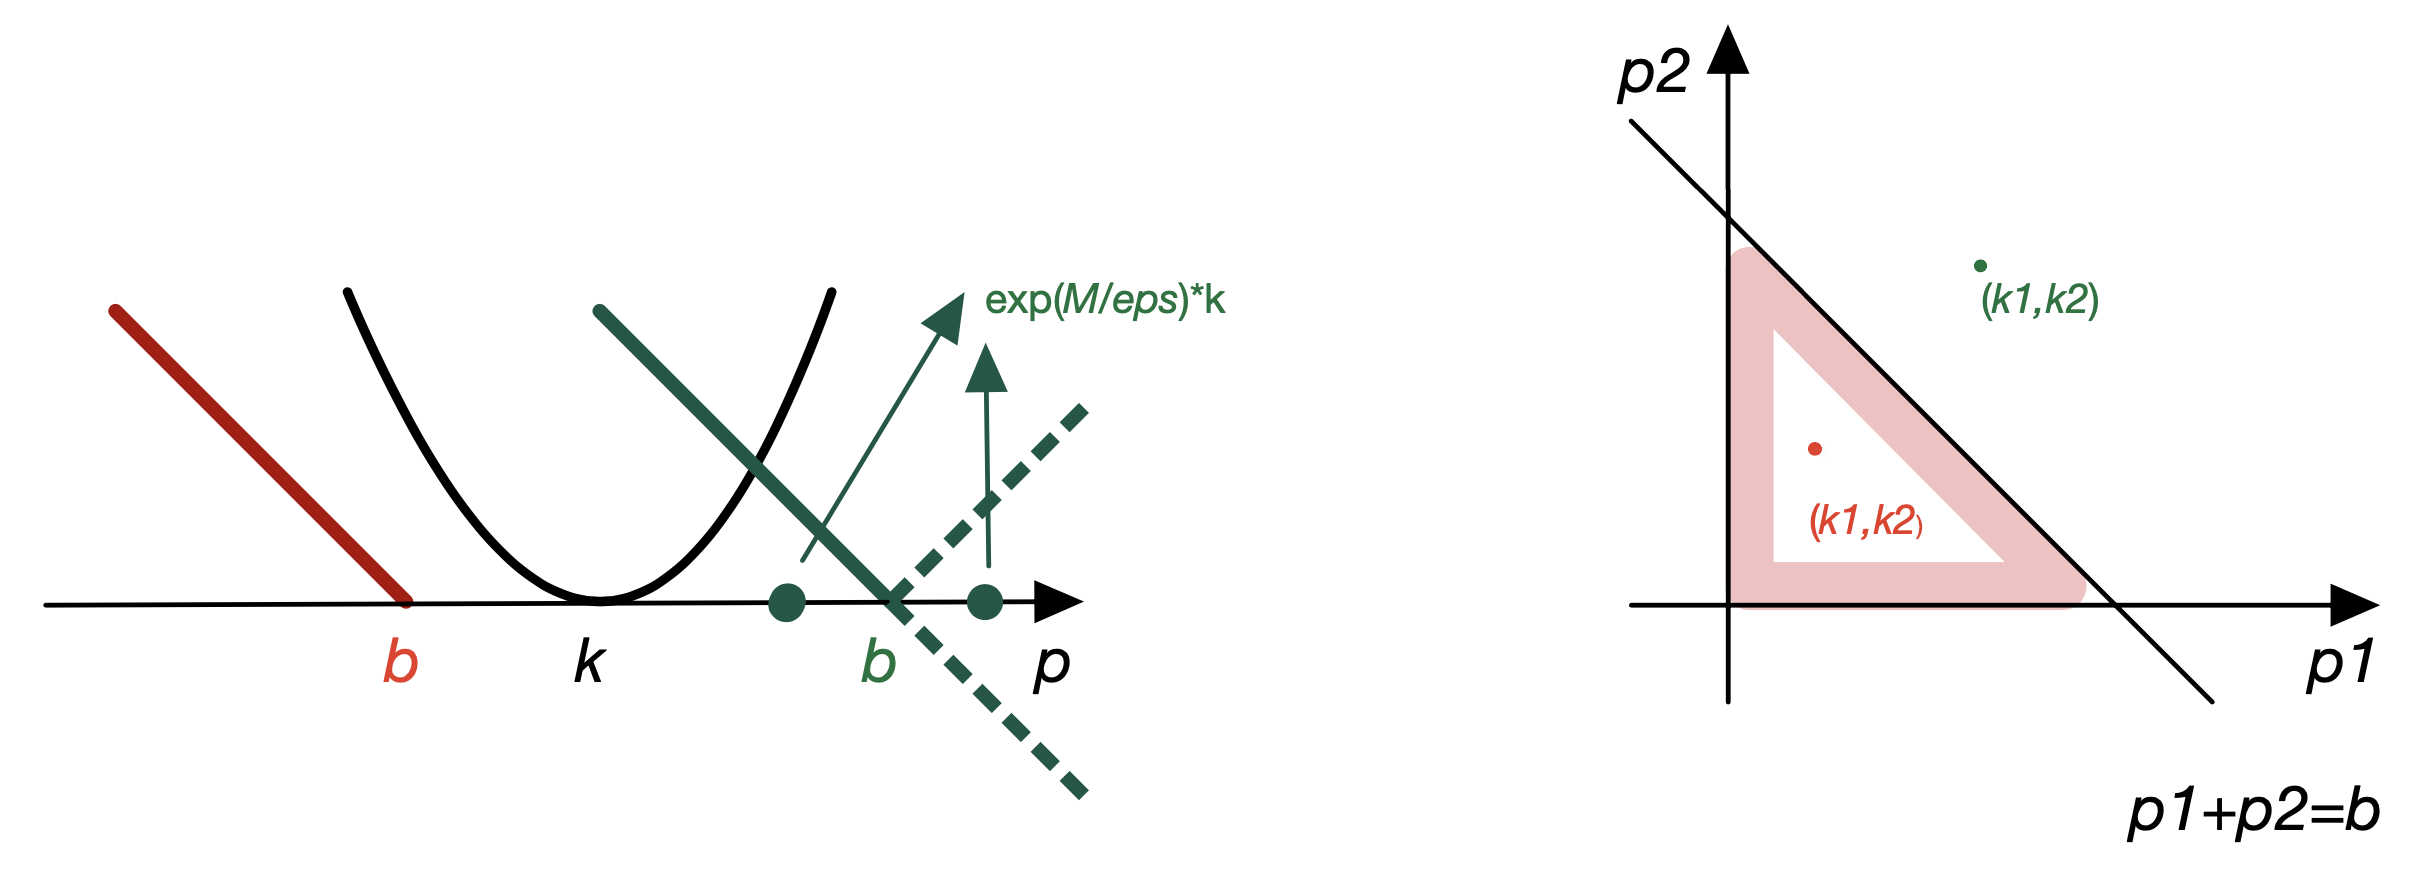
\includegraphics[width=130mm]{Figures/OT_min.png}
\end{center}
\caption{\small {Schematic of minimization of Lemma \ref{lemma:OT_min} for scalar case and Lemma \ref{lemma:OT_min} for vector case. }} 
\label{fig:min_schematic}
\end{figure} 




\begin{lemma}\label{lemma:OT_min}
The following scalar minimization problem has the solution:
\begin{align}
    \underset{p\le b}{\mathrm{argmin}}\ \epsilon\mathrm{KL}(p|k) + M \| p-b \|_1 = \min\{ ke^{\frac{M}{\epsilon}}, b \}.
\end{align}
\end{lemma}
\begin{proof}
If $b\le k$, the minimum is attained at $p^*=b$ because both $\mathrm{KL}(p|k)$ and $\|p-b\|_1$ are decreasing functions over the domain $p\le b$. If $k<b$, then taking the first order optimality condition gives 
\[
\epsilon \log \frac{p}{k} - M = 0 \Rightarrow p = e^{\frac{M}{\epsilon}}k.
\] 
If $e^{\frac{M}{\epsilon}}k \le b$, then the minimum is attained at $p^* = e^{\frac{M}{\epsilon}}k$.; on the other hand, if $e^{\frac{M}{\epsilon}}k > b$, it indicates that the objective function keeps decreasing over the domain $p<b$ (and even beyond, until $e^{\frac{M}{\epsilon}}k$ for $\epsilon\mathrm{KL}(p|k) + M (p-b)$, therefore minimum is reached at $p^* = b$. A summary of the discussion leads to the conclusion. See a schematic of the proof in Figure \ref{fig:min_schematic}.
\end{proof}


\begin{corollary}
The following scalar minimization problem has the solution:
\begin{align}
    \underset{p\ge0}{\mathrm{argmin}}\ \epsilon\mathrm{KL}(p|k) + M \| p - b \|_1 = \min \left\{ ke^{\frac{M}{\epsilon}}, \max \left\{ke^{-\frac{M}{\epsilon}}, b \right\} \right\}.
\end{align}
\end{corollary}



The lemma above can be extended into vector case as follows,
\begin{lemma}\label{lemma:OT_min02}
Let $\mathbf{p}, \mathbf{k}\in\mathbb{R}_+^n$, then
\begin{align}
    \underset{\mathbf{P}^{\mathrm{T}}\mathbb{1}\le \mathbf{b}}{\mathrm{argmin}}\ \epsilon\mathrm{KL}(\mathbf{p}|\mathbf{k}) + M \| \mathbf{p}^{\mathrm{T}}\mathbb{1}-\mathbf{b} \|_1 = \min \left\{ e^{\frac{M}{\epsilon}}, \frac{b}{\mathbf{k}^{\mathrm{T}}\mathbb{1}}  \right\} \mathbf{k}.
\end{align}
\end{lemma}
\begin{proof}
The proof is similar as that of the previous one. If $\mathbf{k}$ is beyond the domain $\mathbf{p}^{\mathrm{T}}\mathbb{1}\le \mathbf{b}$, both $\epsilon\mathrm{KL}(\mathbf{p}|\mathbf{k})$ and $M \| \mathbf{p}^{\mathrm{T}}\mathbb{1}-\mathbf{b} \|_1 $ are convex, and the minimal point $\mathbf{p} = e^{\frac{M}{\epsilon}}\mathbf{k}$ is also beyond the domain $\mathbf{p}^{\mathrm{T}}\mathbb{1}\le b$, then the minimum is attained on the domain boundary $\mathbf{p}^{\mathrm{T}}\mathbb{1} = \mathbf{b}$. Minimizing $\epsilon\mathrm{KL}(\mathbf{p}|\mathbf{k})$ over $\mathbf{p}^{\mathrm{T}}\mathbb{1} = \mathbf{b}$ yields $\mathbf{p}^* = \frac{\mathbf{k}}{\mathbf{k}^{\mathrm{T}}\mathbb{1}}\mathbf{b}$. 

On the other hand, if $\mathbf{k}$ is in the domain $\mathbf{p}^{\mathrm{T}}\mathbb{1} \le \mathbf{b}$, namely, $\mathbf{k}^{\mathrm{T}}\mathbb{1}\le \mathbf{b}$, then we get the minimal point $\mathbf{p}^* = e^{\frac{M}{\epsilon}}\mathbf{k}$ of $\epsilon\mathrm{KL}(\mathbf{p}|\mathbf{k}) + M  ( \mathbf{p}^{\mathrm{T}}\mathbb{1}-\mathbf{b} )$. If it is also in the domain $\mathbf{p}^{\mathrm{T}}\mathbb{1}\le \mathbf{b}$, then it is the expected minimizer $\mathbf{p}^* = e^{\frac{M}{\epsilon}}\mathbf{k}$; on the other hand, if $\mathbf{p}^{*,\mathrm{T}}\mathbb{1} = e^{\frac{M}{\epsilon}}\mathbf{k}^{\mathrm{T}}\mathbb{1} > \mathbf{b}$, the minimum of the original problem is reached on the domain boundary, leading to $\mathbf{p}^* = \frac{\mathbf{k}}{\mathbf{k}^{\mathrm{T}}\mathbb{1}}\mathbf{b}$. Proof is completed.
\end{proof}

We can further extend the conclusion to matrix case.
\begin{lemma}
Let $\mathbf{P}, \mathbf{K}\in\mathbb{R}_+^{n\times n}, \mathbf{a}, \mathbf{b}\in\mathbb{R}_+^n$, the following minimization problems have the solutions:
\begin{align}
& \underset{\mathbf{P}\mathbb{1} \leq \mathbf{a}}{\mathrm{argmin}}\ \epsilon\mathrm{KL}(\mathbf{P}|\mathbf{K}) + M \| \mathbf{P}\mathbb{1} -\mathbf{a} \|_1 = \emph{diag}\left(\min\left\{ \frac{\mathbf{a}}{\mathbf{K}\mathbb{1}}, e^{\frac{M}{\epsilon}}\mathbb{1} \right\} \right) \mathbf{K}, \\
&\underset{\mathbf{P}^{\mathrm{T}}\mathbb{1}\le \mathbf{b}}{\mathrm{argmin}}\ \epsilon\mathrm{KL}(\mathbf{P}|\mathbf{K}) + M \| \mathbf{P}^{\mathrm{T}}\mathbb{1} -\mathbf{b} \|_1 = \mathbf{K} \emph{diag}\left(\min\left\{ \frac{\mathbf{b}}{\mathbf{K}^{\mathrm{T}}\mathbb{1}}, e^{\frac{M}{\epsilon}}\mathbb{1} \right\} \right).
\end{align}
\end{lemma}



Now using the idea of Lemma \ref{lemma:OT_min02}, we can compute the proximal operators $\mathrm{prox}_{\psi_i}^{\epsilon\mathrm{KL}}(\cdot)$ which is summarized in the following lemma.

\begin{lemma}\label{lemma:prox_OptionI}
    Let $\psi_i(\cdot) = \gamma \|\mathbf{a}_i-\cdot\|_1 + \iota_{[0,\mathbf{a}_i]}(\cdot), i = 1, 2$ with $\mathbf{a}_1=\mathbf{a}$ and $\mathbf{a}_2 = \mathbf{b}$, then the proximal operator of $\psi_i$ with respect the $\mathrm{KL}$ divergence is given as
    \begin{align}
    \mathrm{prox}_{\psi_i}^{\epsilon\mathrm{KL}} (\mathbf{q}) = \min\{e^{\gamma/\epsilon}\mathbf{q}, \mathbf{a}_i\}, \ i = 1, 2.
    \end{align}
\end{lemma}

\begin{proof}
    By definition of the proximal operator with respect to the KL divergence, we have
    \begin{align*}
    \mathrm{prox}_{\gamma\|\textbf{a}_i-\cdot\| + \iota_{[0,\textbf{a}_i]}(\cdot)}^{\epsilon\mathrm{KL}}(\mathbf{q}) &= 
    \underset{\mathbf{p}\in[0,\mathbf{a}_i]}{\mathrm{argmin}}\ \epsilon\mathrm{KL}(\mathbf{p}|\mathbf{q}) + \gamma\|\textbf{a}_i-\textbf{p}\|
    \end{align*}
    If $\mathbf{a}_i\le \mathbf{q}$, both $\mathrm{KL}(\cdot|\mathbf{q})$ and $\|\mathbf{a}_i-\cdot\|$ decrease over domain $[0,\mathbf{a}_i]$, so the minimum is attained at $\mathbf{p} = \mathbf{a}_i$; if $\mathbf{a}_i \ge \mathbf{q}$, taking the derivative of $\epsilon\mathrm{KL}(\mathbf{p}|\mathbf{q}) + \gamma\|\mathbf{a}_i-\mathbf{p}\|$ with respect to $\mathbf{p}$ and set it to zero, we find $\mathbf{p} = \min\{e^{\gamma/\epsilon}\mathbf{q}, \mathbf{a}_i\}$. Combining both two cases yields the result.
\end{proof}

Inserting Lemma \ref{lemma:prox_OptionI} to the general Dykstra algorithm for KL divergence (\ref{eqn:generalSinkhorn}), we obtain the generalized Sinkhorn iteration for entropic sOT: Given $\textbf{u}^0 = \textbf{v}^0 = \mathbb{1}$, for any $k=0,1,2,\cdots$, execute the following steps:
\begin{align}
\textbf{u}^{(\ell+1)} &=  \frac{\min\{ e^{\gamma/\epsilon}\textbf{K}\textbf{v}^{(\ell)}, \textbf{a}\}}{\textbf{K} \textbf{v}^{(\ell)}} = \min \left\{ e^{\frac{\gamma}{\epsilon}}\mathbb{1}, \frac{\textbf{a}}{\textbf{K}\textbf{v}^{(\ell)}} \right\}; \\
\textbf{v}^{(\ell+1)} &=  \frac{\min\{ e^{\gamma/\epsilon}\textbf{K}^{\mathrm{T}}\textbf{u}^{(\ell+1)}, \textbf{b}\}}{\textbf{K}^{\mathrm{T}} \textbf{u}^{(\ell+1)}} = \min \left\{ e^{\frac{\gamma}{\epsilon}}\mathbb{1}, \frac{\textbf{b}}{\textbf{K}^{\mathrm{T}}\textbf{u}^{(\ell+1)}} \right\}.
\end{align}







\section{Wassertein Barycenter}


A entropy regularized Wasserstein Barycenter problem can be formulated as:
\begin{align}
\min_{(\mathbf{P}_k)} \left\{ \sum_k \lambda_k \epsilon \mathrm{KL}(\mathbf{P}_k|\mathbf{K}): \forall k, \mathbf{P}_k^{\mathrm{T}}\mathbb{1} = \mathbf{b}_k, \mathbf{P}_k \mathbb{1} = \mathbf{a}, \text{ for some } \mathbf{a}\right\}.
\end{align}

In \cite{benamou2015augmented}, an algorithm is proposed as:
\begin{align}
\mathbf{v}_k^{(n+1)} &= \frac{\mathbf{b}_k}{\mathbf{K}^T\mathbf{u}_k^{(n)}}; \\
\mathbf{u}_k^{(n+1)} &= \frac{\mathbf{a}^{(n+1)}}{\mathbf{K}\mathbf{v}_k^{(n+1)}}, \quad \mathbf{a}^{(n+1)} = \prod_k ({\color{red}\mathbf{u}_k^{(n)}}\odot\mathbf{K}\mathbf{v}_k^{(n+1)})^{\lambda_k}.  \label{eqn:Benamou02}
\end{align}
However in \cite{peyre2019computational}, an alternative algorithm is proposed as:
\begin{align}
\mathbf{v}_k^{(n+1)} &= \frac{\mathbf{b}_k}{\mathbf{K}^T\mathbf{u}_k^{(n)}}; \label{eqn:Cuturi01}\\
\mathbf{u}_k^{(n+1)} &= \frac{\mathbf{a}^{(n+1)}}{\mathbf{K}\mathbf{v}_k^{(n+1)}}, \quad \mathbf{a}^{(n+1)} = \prod_k (\mathbf{K}\mathbf{v}_k^{(n+1)})^{\lambda_k}.\label{eqn:Cuturi02}
\end{align}
why there is a difference indicated by ${\color{red}\mathbf{u}_k^{(n)}}$?

Benamou's algorithm is derived by Bregman iteration. Let 
\begin{align}
\mathcal{C}_1 = \{\mathbf{P} = (\mathbf{P}_k) : \mathbf{P}_k \mathbb{1} = \mathbf{a}, \text{ for some } \mathbf{a}\}, \quad
\mathcal{C}_2 = \{\mathbf{P} = (\mathbf{P}_k) : \mathbf{P}_k^{\mathrm{T}}\mathbb{1} = \mathbf{b}_k\}.
\end{align}
Then we have
\begin{align*}
\mathbf{P}^{(2n+1)} &= \text{proj}_{\mathcal{C}_1}^{\mathrm{KL}_{\lambda}}(\mathbf{P}^{(2n)}) \\
& = \min_{\tilde{\mathbf{P}}\in\mathcal{C}_1} \epsilon \mathrm{KL}_{\lambda}(\tilde{\mathbf{P}}|\mathbf{P}^{(2n)}) \\
& = \min_{\tilde{\mathbf{P}}, a} \sum_k \lambda_k \left[ \epsilon\mathrm{KL}\left(\tilde{\mathbf{P}}_k|\mathbf{P}^{(2n)}_k\right) - \left\langle \mathbf{f}_k , \tilde{\mathbf{P}}_k \mathbb{1} - \mathbf{a} \right\rangle \right].
\end{align*}
Taking the first order optimality condition:
\begin{align*}
& \frac{\partial}{\partial (\tilde{\mathbf{P}}_k)_{ij}} \quad \Rightarrow \quad \epsilon \log \frac{(\tilde{\mathbf{P}}_k)_{ij}}{(\mathbf{P}^{(2n)}_k)_{ij}} - (\mathbf{f}_k)_i = 0 \quad \Rightarrow \quad \tilde{\mathbf{P}}_k = \text{diag}(e^{\frac{\mathbf{f}_k}{\epsilon}})\mathbf{P}_k^{(2n)}; \\
&\frac{\partial}{\partial \mathbf{a}_{i}}  \quad \Rightarrow \quad \sum_k \lambda_k (\mathbf{f}_k)_i = 0 \quad \Rightarrow \quad \sum \lambda_k \mathbf{f}_k = 0.
\end{align*}
The row sum condition results in:
\begin{align*}
\tilde{\mathbf{P}}_k \mathbb{1} = \mathbf{a} & \quad \Rightarrow \quad  e^{\frac{\mathbf{f}_k}{\epsilon}} \odot \mathbf{P}_k^{(2n)} \mathbb{1} = \mathbf{a} \\
& \quad \Rightarrow \quad \frac{\mathbf{f}_k}{\epsilon} + \log(\mathbf{P}_k^{(2n)} \mathbb{1}) = \log \mathbf{a} \\
& \quad \Rightarrow \quad \sum_k \lambda_k\frac{\mathbf{f}_k}{\epsilon} + \sum_k \lambda_k \log(\mathbf{P}_k^{(2n)} \mathbb{1}) = \sum_k \lambda_k \log \mathbf{a} \\
& \quad \Rightarrow \quad \mathbf{a} = \prod_k \left(\mathbf{P}_k^{(2n)} \mathbb{1}\right)^{\lambda_k}.
\end{align*}
Hence the update on $\mathbf{u}_k = e^{\frac{\mathbf{f}_k}{\epsilon}} = \frac{\mathbf{a}}{\mathbf{P}_k^{(2n)} \mathbb{1}}$, obtained from
\[
\mathbf{P}_k^{(2n+1)} = \text{diag} \left(\mathbf{u}_k^{(2n+1)} \right) \mathbf{K}  \text{diag} \left(\mathbf{v}_k^{(2n+1)}\right) = \text{diag} \left(  e^{\frac{\mathbf{f}_k}{\epsilon}} \right) \text{diag}\left(\mathbf{u}_k^{(2n)} \right) \mathbf{K}  \text{diag} \left(\mathbf{v}_k^{(2n)}\right),
\]
reads
\[
\mathbf{u}_k^{(2n+1)} =  e^{\frac{\mathbf{f}_k}{\epsilon}} \odot \mathbf{u}_k^{(2n)} = \frac{\mathbf{a}}{\mathbf{P}_k^{(2n)}1} \odot \mathbf{u}_k^{(2n)}
= \frac{\prod_k \left( \mathbf{u}_k^{(2n)}\odot \mathbf{K}\mathbf{v}_k^{(2n)} \right)^{\lambda_k}}{\mathbf{K}\mathbf{v}_k^{(2n)}} 
\]
which is identical to the equation (\ref{eqn:Benamou02}).

On the other hand, the alternative algorithm in (\ref{eqn:Cuturi01})-(\ref{eqn:Cuturi02}) is obtained from considering directly the steady state equation of the dual form. According to the dual form
\begin{align}
\max_{(\mathbf{f}_k),(\mathbf{g}_k)}  \left\{ \sum_k \lambda_k \left[ \langle \mathbf{g}_k, \mathbf{b}_k \rangle - \epsilon \left \langle e^{\frac{1}{\epsilon}(-\mathbf{C}+\mathbf{f}\oplus\mathbf{g})}, \mathbb{1} \right \rangle   \right] : \sum_k \lambda_k \mathbf{f}_k = 0 \right\},
\end{align}
we have
\begin{align*}
\max_{(\mathbf{f}_k),(\mathbf{g}_k)}  \sum_k \lambda_k \left[ \langle \mathbf{g}_k, \mathbf{b}_k \rangle - \epsilon \left \langle e^{\frac{1}{\epsilon}(-\mathbf{C}+\mathbf{f}\oplus\mathbf{g})}, \mathbb{1} \right \rangle   \right] 
+ \left\langle \sum_{k} \lambda_k\mathbf{f}_k , \mathbf{a} \right\rangle.
\end{align*}
Differentiating the objective function with respect to $\mathbf{f}_k$ arrives:
\begin{align*}
-\lambda_k e^{\frac{\mathbf{f}_k}{\epsilon}} \odot \mathbf{K} e^{\frac{\mathbf{g}_k}{\epsilon}} + \lambda_k \mathbf{a} = 0.
\end{align*}
The same idea applies on the above equation to get the steady state equation:
\begin{align*}
\mathbf{a} = \prod_k (\mathbf{K}e^{\frac{\mathbf{g}_k}{\epsilon}})^{\lambda_k}, \quad e^{\frac{\mathbf{f}_k}{\epsilon}} = \frac{\prod_k (\mathbf{K}e^{\frac{\mathbf{g}_k}{\epsilon}})^{\lambda_k}}{\mathbf{K}e^{\frac{\mathbf{g}_k}{\epsilon}}},
\end{align*}
or equivalently using primal variables $(\mathbf{u},\mathbf{v})$ to obtain:
\begin{align}\label{eqn:dual01}
\mathbf{a} = \prod_k (\mathbf{K}\mathbf{v}_k)^{\lambda_k},
\quad \mathbf{u}_k = \frac{\mathbf{a}}{\mathbf{K}\mathbf{v}_k}.
\end{align}
The other steady state equation obtained from differentiating the objective function with respect to $\mathbf{g}_k$ is:
\begin{align}\label{eqn:dual02}
e^{\frac{\mathbf{g}_k}{\epsilon}} \odot \mathbf{K}^T e^{\frac{\mathbf{f}_k}{\epsilon}}  = \mathbf{b}_k.
\end{align}
Applying alternating minimization on the dual problem based on steady state equations (\ref{eqn:dual01})-(\ref{eqn:dual02}) leads to the algorithm (\ref{eqn:Cuturi01})-(\ref{eqn:Cuturi02}).








\chapter[Dynamical OT]{Dynamical Optimal Transport: Theories}\label{chapter:DOT}



The goal of this chapter is to introduce a differential structure on the space of probability measures, starting from the Benamou--Brenier formula and then introducing Otto's formalism. This will allow us to interpret several important PDEs as gradient flows with respect to the 2-Wasserstein distance. In order to focus on the main ideas behind this important theory, most computations in this chapter will be formal.

In the previous chapter, we saw that, considering the entropy functional 
$
\rho \mapsto \int \rho \log(\rho)
$
in the 2-Wasserstein space, the discrete Euler scheme for gradient flows produces solutions to the heat equation. It is natural to wonder whether we can say that, in some sense,

\begin{center}
\textit{the heat equation is the gradient flow of the entropy with respect to the $W_2$ metric.}
\end{center}

Moreover, one might ask whether a similar strategy could handle other evolution equations. In this chapter, we give an answer to these questions by endowing the Wasserstein space with a differential structure. This makes it much easier to guess (and, with the right toolbox, prove) that the gradient flow of the entropy is the heat equation. Also, this will allow us to repeat the same strategy for other functionals/evolution equations.

\section[Benamou-Brenier]{The Continuity Equation and Benamou--Brenier Formula}

Let $\Omega \subset \mathbb{R}^d$ be a convex set ($\Omega = \mathbb{R}^d$ is admissible). Throughout, we commit a mild abuse of notation and identify all probability measures with their densities: $\text{d}\rho(\mathbf{x}) = \rho(\mathbf{x})\text{d}\mathbf{x}$. In other words, when we have two probability densities $\rho_1$ and $\rho_2$, their $p$-Wasserstein distance means the $p$-Wasserstein distance between the two measures $\rho_1\text{d}\mathbf{x}, \rho_2\text{d}\mathbf{x}$:
\begin{align*}
	W_p(\rho_1,\rho_2): = W_p(\rho_1 \text{d}\mathbf{x}, \rho_2 \text{d}\mathbf{x}).
\end{align*}
Let $\mu \in \mathcal{P}_2(\Omega)$ be a probability measure with finite second moments, and let $\mathbf{v} : [0, T] \times \Omega \to \mathbb{R}^d$ be a smooth bounded vector field tangent to the boundary of $\Omega$. Let $\mathbf{X}(t, \mathbf{x})$ denote the flow of $\mathbf{v}$, namely
\begin{align}\label{eqn:dynamicalOT_velocity_flow}
\begin{cases}
    \dot{\mathbf{X}}(t, \mathbf{x}) = \mathbf{v}(t, \mathbf{X}(t, \mathbf{x})), \\
    \mathbf{X}(0, \mathbf{x}) = \mathbf{x},
\end{cases}
\end{align}
and set $\rho(t,\cdot) = (\mathbf{X}(t))_\sharp \mu$. Note that, since $\mathbf{v}$ is tangent to the boundary, the flow remains inside $\Omega$, hence $\rho(t,\cdot) \in \mathcal{P}_2(\Omega)$.

\begin{lemma}\label{lemma:continuity_eqn}
Let $\mathbf{v}_t(\cdot) := \mathbf{v}(t, \cdot)$ and $\rho_t(\cdot) := \rho(t, \cdot)$ (the two notations are interchangeable hereafter). The continuity equation
\begin{align}\label{eqn:continuity}
\partial_t \rho_t + \nabla\cdot(\rho_t \mathbf{v}_t) = 0
\end{align}
holds in the distributional sense.
\end{lemma}

\begin{proof}
Let $\psi \in C_c^\infty(\Omega)$, and consider the function $t \mapsto \int_\Omega \rho_t(x) \psi(x) \, dx$. Then, using the definitions of $\mathbf{X}$ and $\rho_t$, we get
\begin{align*}
\int_\Omega \partial_t \rho_t(\mathbf{x}) \psi(\mathbf{x}) \, \text{d}\mathbf{x} = &\frac{\text{d}}{\text{d}t} \int_\Omega \rho_t(\mathbf{x}) \psi(\mathbf{x}) \, \text{d}\mathbf{x} = \frac{\text{d}}{\text{d}t} \int_\Omega \psi(\mathbf{X}(t,\mathbf{x})) \mu(\mathbf{x}) \, \text{d}\mathbf{x} \\
=& \int_\Omega \nabla \psi(\mathbf{X}(t, \mathbf{x})) \cdot \dot{\mathbf{X}}(t, \mathbf{x}) \mu(\mathbf{x}) \, \text{d}\mathbf{x} \\
=& \int_\Omega \nabla \psi(\mathbf{X}(t, \mathbf{x})) \cdot \mathbf{v}_t(\mathbf{X}(t, \mathbf{x})) \mu(\mathbf{x}) \, \text{d}\mathbf{x} \\
=& \int_\Omega \nabla \psi(\mathbf{x}) \cdot \mathbf{v}_t(\mathbf{x}) \rho_t(\mathbf{x}) \, \text{d}\mathbf{x} = -\int_\Omega \psi(\mathbf{x}) \, \nabla\cdot(\rho_t \mathbf{v}_t) \, \text{d}\mathbf{x},
\end{align*}
which implies the continuity equation.
\end{proof}

\begin{definition}
Given a pair $(\rho_t, \mathbf{v}_t)$ solving the continuity equation (\ref{eqn:continuity}), with $\mathbf{v}_t \cdot \mathbf{n}|_{\partial \Omega} = 0$ (namely, $\mathbf{v}_t$ is tangent to the boundary of $\Omega$), the dynamical optimal transport is defined as
\begin{align}\label{eqn:dynamicalOT02}
    C_{\mathrm{BB}}(\mu,\nu) = \min_{(\rho,\mathbf{v})\in\mathcal{C}_{\mathrm{BB}}}\  A[\rho_t, \mathbf{v}_t] = \int_0^1\int_{\Omega} \rho_t(\mathbf{x}) \|\mathbf{v}_t(\mathbf{x})\|^2 \ \dx\dt,
\end{align}
where we define the set of constraints as
\begin{align}
    \mathcal{C}_{\mathrm{BB}}(\mu,\nu) : = \left\{ (\rho_t,\mathbf{v}_t) | \partial_t\rho_t = -\nabla\cdot(\rho_t \mathbf{v}_t),\ \rho(0,\mathbf{x})=\mu,\ \rho(1,\mathbf{x})=\nu,\ \mathbf{v}\cdot \mathbf{n}|_{\partial \Omega} = 0  \right\}.
\end{align}
\end{definition}

The following remarkable formula, due to Benamou and Brenier \cite{benamou2000computational} (hence the notation $C_{\mathrm{BB}}$), shows a link between the continuity equation and the $W_2$-distance.

\begin{theorem}[Benamou--Brenier Theorem]\label{theorem:BB}
Given two probability measures $\mu, \nu \in \mathcal{P}_2(\Omega)$, it holds that
\begin{align}\label{eqn:dynamicalOT}
W_2^2(\mu, \nu) = C_{\mathrm{BB}}(\mu,\nu).
\end{align}
\end{theorem}

\begin{proof}
We give only a formal proof.

Let $(\rho_t, \bv_t)$ be a couple (probability measure/smooth vector field) satisfying $\rho_0 = \mu, \rho_1 = \nu$, and $\partial_t \rho_t + \nabla\cdot(\rho_t \bv_t) = 0$. Let $\mathbf{X}(t, \mathbf{x})$ denote the flow of $\mathbf{v}_t$. By the uniqueness for the continuity equation, the unique solution $\rho_t$ is the one constructed in Lemma \ref{lemma:continuity_eqn}, namely $\rho_t = (\mathbf{X}(t))_\sharp \mu$. In particular, $\mathbf{X}(1)_\sharp \mu = \nu$, which implies that $\mathbf{X}(1,\mathbf{x})$ is a transport map from $\mu$ to $\nu$. Then by the definition of $\mathbf{X}$ and Holder inequality, we get
\begin{align}
A[\rho_t, v_t] &= \int_0^1 \int_{\Omega} \|\mathbf{v}_t(\mathbf{x})\|_2^2 \rho_t(\mathbf{x}) \, \dx\dt \nonumber\\
&= \int_0^1 \int_{\Omega} \|\mathbf{v}_t(\mathbf{X}(t,\mathbf{x}))\|_2^2 \ \mu(\mathbf{x}) \, \dx\dt = \int_{\Omega} \left[ \int_0^1 \|\dot{\mathbf{X}}(t,\mathbf{x})\|_2^2 \ \mu(\mathbf{x}) \, \dt \right] \dx \\
&= \int_{\Omega} \mu(\mathbf{x}) \int_0^1 \|\dot{\mathbf{X}}(t,\mathbf{x})\|_2^2 \ \dt\ \dx 
\geq \int_{\Omega} \mu(\mathbf{x}) \left(\int_0^1 \dot{\mathbf{X}}(t,\mathbf{x}) \, \dt \right)^2 \, \dx \nonumber \\
&= \int_{\Omega}  |\mathbf{X}(1,\mathbf{x}) - \mathbf{x}|^2 \mu(\mathbf{x})\, \dx \geq W^2_2(\mu, \nu). \nonumber
\end{align}
Hence, this proves that $W^2_2(\mu, \nu)$ is always less than or equal to the infimum appearing in the statement.

On the other hand, take \( \mathbf{X}(t,\mathbf{x}) = \mathbf{x} + t(\mathbf{T}(\mathbf{x}) - \mathbf{x}) \), where \( \mathbf{T} \) is the optimal Monge map from \( \mu \) to \( \nu \), set \( \rho_t := (\mathbf{X}_t)_\sharp \mu \) and let \( \mathbf{v}_t \) be such that \( \dot{\mathbf{X}} = \mathbf{v}_t \circ \mathbf{X}_t \). With this choice we have \( \dot{\mathbf{X}}(t,\mathbf{x}) = \mathbf{T}(\mathbf{x}) - \mathbf{x} = \mathbf{v}_t(\mathbf{X}(t,\mathbf{x})) \), and looking at the computations above one can easily check that all inequalities in (4.2) become equalities, therefore we have
\[
\inf A[\rho_t, v_t] \le A[\rho_t, v_t] = W_2^2(\mu,\nu).
\]
Finally we have
\[
\inf A[\rho_t, v_t] = W^2_2(\mu, \nu).
\]
The equivalence is obtained.
\end{proof}


The proof of the Benamou-Brenier theorem indeed provides an explicit relation between the optimal Monge map $\mathbf{T}^*(\mathbf{x})$ and the optimal $(\rho^*, \mathbf{v}^*)$.
\begin{corollary}
    Let $\mathbf{T}^*$ be the optimal Monge map from $\mu$ to $\nu$, then the optimal solution $(\rho^*, v^*)$ of the dynamical OT (\ref{eqn:dynamicalOT}) can be constructed as below: Take $\mathbf{X}(t,\mathbf{x}) = (1-t)\mathbf{x}+t\mathbf{T}^*(\mathbf{x})$, then
    \begin{align*}
        \rho^*(t,\mathbf{x})=(\mathbf{X}_t)_{\sharp}\mu, \quad \mathbf{v}^*(t,\mathbf{x}) = \dot{\mathbf{X}}\circ(\mathbf{X}_t^{-1}) = (\mathbf{T}^*-\emph{Id})\circ \mathbf{X}_t^{-1} = \mathbf{T}^*(\mathbf{X}_t^{-1}(\mathbf{x})) - \mathbf{X}_t^{-1}(\mathbf{x}).
    \end{align*}
    Reversely, given the optimal solution $(\rho^*, \mathbf{v}^*)$ of the dynamical OT (\ref{eqn:dynamicalOT}), the optimal Monge map $\mathbf{T}^*$ can be constructed as follows:
    \begin{align*}
        \mathbf{T}^*(\mathbf{x}) = \mathbf{x} + \mathbf{v}^*_t(\mathbf{X}(t,\mathbf{x})) = \mathbf{x} + \mathbf{v}^*_0(\mathbf{X}(0,\mathbf{x})) = \mathbf{x} + \mathbf{v}^*(0,\mathbf{x}).
    \end{align*}
\end{corollary}






\section[Straight Trajectories]{Dynamical OT Induces Straight Trajectories}

In this section, we discuss in further more detail about the relations between dynamical OT and the static OT. 

First of all, the Benamou-Brenier OT formulation \eqref{eqn:dynamicalOT02} can be reformulated as a convex problem with linear constraint as follows
\begin{align}\label{eqn:dynamicalOT03}
    C_{\mathrm{BB}}(\mu,\nu) =  &\min_{(\rho_t,\mathbf{m}_t)\in\mathcal{C}_{\mathrm{BB}}}\  A[\rho_t, \mathbf{m}_t] = \int_0^1\int_{\Omega} J(\rho_t, \mathbf{m}_t) \ \dx\dt,
\end{align}
with linearly constrained feasible set
\begin{align}
    \mathcal{C}_{\mathrm{BB}}(\mu,\nu) : = \left\{ (\rho_t,\mathbf{m}_t) |\ \partial_t\rho_t + \nabla\cdot \mathbf{m}_t = 0,\ \rho(0,\mathbf{x})=\mu,\ \rho(1,\mathbf{x})=\nu,\ \mathbf{m}\cdot \mathbf{n}|_{\partial \Omega} = 0  \right\}.
\end{align}
Here $J$ is the lower semi-continuous convex function
\begin{align}\label{eqn:J_definition02}
  J(\rho_t,\mathbf{m}_t) = 
  \begin{cases}
    \rho_t^{-1}\|\mathbf{m}_t\|_2^2 \quad &\text{if\ } \rho >0, \\
    0 \quad &\text{if\ } (\rho_t, \mathbf{m}_t) = (0,0), \\
    +\infty, \quad & \text{otherwise}.
  \end{cases}
\end{align}
Here we employ a slight abuse of notation with $A[\rho_t,\mathbf{m}_t]$ and $\mathcal{C}(\mu,\nu)$. This rewrite is crucial for the numerical treatment for the Benamou-Brenier OT \eqref{eqn:dynamicalOT02}. Besides, it is also the key for proving the existence of the minimizers for Benamou-Brenier.

Now for can present the dual formulation for the Benamou-Brenier.

\begin{proposition}[Dual form of Benamou-Brenier]
    The minimizer $(\rho,\mathbf{v})$ of the Benamou-Brenier dynamical OT \eqref{eqn:dynamicalOT02} satisfies
    \begin{align*}
        \mathbf{v}(t,\mathbf{x}) = \nabla\Phi(t,\mathbf{x})
    \end{align*}
    in which the dual variable $\Phi(t,\mathbf{x})$ is determined by
    \begin{align}\label{eqn:BB_dualsystem}
        \begin{cases}
         \partial_t\rho(t,\mathbf{x}) + \nabla\cdot(\rho(t,\mathbf{x})\nabla\Phi(t,\mathbf{x})) = 0, \\
         \partial_t\Phi(t,\mathbf{x}) + \dfrac{1}{2}\|\nabla\Phi(t,\mathbf{x})\|_2^2 \le 0, \\
         \rho(0,\mathbf{x}) = \mu, \quad \rho(1,\mathbf{x}) = \nu.
        \end{cases}
      \end{align}
      If $\rho(t,\mathbf{x})>0$, then 
      \begin{align}\label{eqn:HJ02}
        \partial_t\Phi(t,\mathbf{x}) + \frac{1}{2}\|\nabla\Phi(t,\mathbf{x})\|_2^2 = 0.
      \end{align}
\end{proposition}
\begin{proof}
    The proof is traightforward. Taking $2\Phi_t(\mathbf{x}) = 2\Phi(t,\mathbf{x})$ as the dual variable and considering the Lagrangian
    \begin{align*}
        \mathcal{L}(\rho,\mathbf{m};\Phi) = \int_0^1\int_{\Omega} \rho_t^{-1}\|\mathbf{m}\|_2^2 + 2\Phi_t\Big(\partial_t\rho(t,\mathbf{x})+\nabla\cdot\mathbf{m}(t,\mathbf{x})\Big)\ \dx\dt.
    \end{align*}
    By the conditions
    \begin{align*}
        &\frac{\delta \mathcal{L}}{\delta \rho}\ge0 \Longrightarrow -\rho_t^{-2}\|\mathbf{m}\|_2^2 - 2\partial_t\Phi_t \ge 0 ; \\
        &\frac{\delta \mathcal{L}}{\delta \mathbf{m}}=0 \Longrightarrow -2\rho_t^{-1}\mathbf{m} -2 \nabla\Phi_t = 0; \\
        &\frac{\delta \mathcal{L}}{\delta \Phi}=0 \Longrightarrow \partial_t\rho(t,\mathbf{x})+\nabla\cdot\mathbf{m}(t,\mathbf{x}),
    \end{align*}
    which recover the required system by using $\nabla\Phi_t = \rho^{-1}\mathbf{m} = \mathbf{v}$. If $\rho_t >0$ strictly, the Hamilton-Jacobi equation has equal sign.
\end{proof}


Now we can provide an alternative derivation of the static Monge formulation from the Benamou-Brenier \eqref{eqn:dynamicalOT02}.
\begin{proposition}
    Given the following static Monge OT
    \begin{align}
        C_{\mathrm{M}}(\mu,\nu) : = \inf \left\{\int_{\Omega}  \mu(\mathbf{x}) \|\mathbf{T}(\mathbf{x}) - \mathbf{x}\|_2^2  \ \dx \mid \mathbf{T}_\sharp \mu = \nu \right\}, 
    \end{align}
    we have that
    \begin{align*}
        C_{\mathrm{M}}(\mu,\nu) = C_{\mathrm{BB}}(\mu,\nu).
    \end{align*}
\end{proposition}
\begin{proof}
    Consider any (smooth) vecocity field and its flow $(\mathbf{v}, \mathbf{X})$ satisfying
    \begin{align}\label{eqn:dynamicalOT_velocity_flow02}
        \begin{cases}
            \dot{\mathbf{X}}(t, \mathbf{x}) = \mathbf{v}(t, \mathbf{X}(t, \mathbf{x})), \\
            \mathbf{X}(0, \mathbf{x}) = \mathbf{x},
        \end{cases}
    \end{align}
    and define $\rho(t,\mathbf{x}) := (\mathbf{X}_t)_{\sharp}\mu(\mathbf{x})$. By Lemma \ref{lemma:continuity_eqn}, $(\rho,\mathbf{v})$ satisfies the continuity equation \eqref{eqn:continuity}. Then we have
    \begin{align}
        \int_0^1 \int_{\Omega} \rho(t,\mathbf{x}) \|\mathbf{v}(t,\mathbf{x})\|_2^2 \ \dx\dt
        &= \int_0^1 \int_{\Omega} \rho(t,\mathbf{X}) \|\mathbf{v}(t,\mathbf{X})\|_2^2 \ \mathrm{d}\mathbf{X}\dt \nonumber\\
        &= \int_0^1 \int_{\Omega}  \|\dot{\mathbf{X}}(t,\mathbf{x})\|_2^2 \ \rho(t,\mathbf{X}) \mathrm{det}(\nabla_{\mathbf{x}}\mathbf{X}) \mathrm{d}\mathbf{x}\dt. \label{eqn:CM_CBB_temp}
    \end{align}
    We next derive a differential equation for the quantity $J(t,\mathbf{x}) = \rho(t,\mathbf{X}_t(\mathbf{x})) \mathrm{det}(\nabla_{\mathbf{x}}\mathbf{X}_t(\mathbf{x}))$. Note that
    \begin{align*}
        \frac{\mathrm{d}}{\mathrm{d}t}J(t,\mathbf{x}) 
       & = \frac{\mathrm{d}}{\mathrm{d}t} \Big[ \rho(t,\mathbf{X}) \mathrm{det}(\nabla_{\mathbf{x}}\mathbf{X}) \Big] \\
       & = \partial_t\rho(t,\mathbf{X}) \mathrm{det}(\nabla_{\mathbf{x}}\mathbf{X}) + \nabla_{\mathbf{X}} \rho(t,\mathbf{X}) \frac{\mathrm{d}\mathbf{X}}{\mathrm{d}t} \mathrm{det}(\nabla_{\mathbf{x}}\mathbf{X}) + \rho(t,\mathbf{X}) \partial_t\Big[ \mathrm{det}(\nabla_{\mathbf{x}}\mathbf{X}) \Big] \\
       & = \Big( \partial_t\rho + \nabla\rho\cdot\mathbf{v} + \rho\nabla\cdot\mathbf{v}  \Big)(t,\mathbf{X}) \mathrm{det}(\nabla_{\mathbf{x}}\mathbf{X}) \\
       & = \Big( \partial_t\rho + \nabla\cdot(\rho\mathbf{v}) \Big)(t,\mathbf{X}) \mathrm{det}(\nabla_{\mathbf{x}}\mathbf{X}) = 0,
    \end{align*}
    where the third equality is due to the Jacobi's formula:
    \begin{align*}
        \partial_t \mathrm{det}(\nabla_{\mathbf{x}}\mathbf{X}) & = \mathrm{det}(\nabla_{\mathbf{x}}\mathbf{X}) \mathrm{tr}\left( (\nabla_{\mathbf{x}}\mathbf{X})^{-1} \frac{\mathrm{d}}{\mathrm{d}t}(\nabla_{\mathbf{x}}\mathbf{X})  \right) = \mathrm{det}(\nabla_{\mathbf{x}}\mathbf{X}) \mathrm{tr}\left( (\nabla_{\mathbf{x}}\mathbf{X})^{-1} \nabla_{\mathbf{x}}\frac{\mathrm{d}\mathbf{X}}{\mathrm{d}t}  \right) \\
        & = \mathrm{det}(\nabla_{\mathbf{x}}\mathbf{X}) \mathrm{tr}\left( (\nabla_{\mathbf{x}}\mathbf{X})^{-1} \nabla_{\mathbf{x}}\mathbf{v}(t,\mathbf{X})  \right) = \mathrm{det}(\nabla_{\mathbf{x}}\mathbf{X}) \mathrm{tr}\left( (\nabla_{\mathbf{x}}\mathbf{X})^{-1} \nabla_{\mathbf{X}}\mathbf{v}(t,\mathbf{X}) \nabla_{\mathbf{x}}\mathbf{X}  \right) \\
        & = \mathrm{det}(\nabla_{\mathbf{x}}\mathbf{X}) \mathrm{tr}\left( \nabla_{\mathbf{X}}\mathbf{v}(t,\mathbf{X}) \nabla_{\mathbf{x}}\mathbf{X} (\nabla_{\mathbf{x}}\mathbf{X})^{-1} \right) = \mathrm{det}(\nabla_{\mathbf{x}}\mathbf{X}) \mathrm{tr}\left( \nabla_{\mathbf{X}}\mathbf{v}(t,\mathbf{X})  \right) \\
        & = \mathrm{det}(\nabla_{\mathbf{x}}\mathbf{X}) \nabla_{\mathbf{X}}\cdot\mathbf{v}(t,\mathbf{X})
    \end{align*}
    Therefore we have 
    $
        J(t,\mathbf{x}) = J(0,\mathbf{x}) = \rho(0,\mathbf{x}) = \mu(\mathbf{x}).
    $
    When $\mathbf{X}$ is the Lagrangian minimizer, the minimizer in Eulerian coordinators satisfies the Hamilton-Jacobi equation \eqref{eqn:HJ02}. This combined with $\dot{\mathbf{X}}=\mathbf{v}(t,\mathbf{X})=\nabla\Phi(t,\mathbf{X})$, we have that
    \begin{align*}
        \ddot{\mathbf{X}}(t,\mathbf{x}) = \frac{\mathrm{d}}{\mathrm{d}t}\nabla\Phi(t,\mathbf{X}) 
        = \partial_t \nabla\Phi(t,\mathbf{X}) + \nabla^2\Phi(t,\mathbf{X}) \frac{\mathrm{d}\mathbf{X}}{\mathrm{d}t} 
         = \nabla_{\mathbf{X}} \partial_t\Phi(t,\mathbf{X}) + \nabla_{\mathbf{X}}\Big( \frac{1}{2}\| \nabla\Phi(t,\mathbf{X}) \|_2^2 \Big) = 0.
    \end{align*}
    This implies that $\dot{\mathbf{X}}$ is a constant with respect to $t$ and
    \begin{align*}
        \dot{\mathbf{X}}=\mathbf{v}(t,\mathbf{X}) = \int_0^1 \dot{\mathbf{X}}\ \dt = \mathbf{X}(1,\mathbf{x}) - \mathbf{X}(0,\mathbf{x}) := \mathbf{T}(\mathbf{x}) - \mathbf{x}.
    \end{align*}
    It follows that 
    \begin{align*}
        \mathbf{X}(t,\mathbf{x}) = t\mathbf{T}(\mathbf{x}) + (1-t)\mathbf{x}.
    \end{align*}
    Substituting all the about equations into \eqref{eqn:CM_CBB_temp}, we have
    \begin{align*}
        \int_0^1 \int_{\Omega} \rho(t,\mathbf{x}) \|\mathbf{v}(t,\mathbf{x})\|_2^2 \ \dx\dt
        & = \int_0^1 \int_{\Omega}  \|\dot{\mathbf{X}}(t,\mathbf{x})\|_2^2 \ J(t,\mathbf{x})\mathrm{d}\mathbf{x}\dt\\
        & = \int_0^1 \int_{\Omega}  \|\mathbf{T}(\mathbf{x})-\mathbf{x}\|_2^2 \ J(0,\mathbf{x})\mathrm{d}\mathbf{x}\dt \\
        & = \int_0^1 \int_{\Omega}  \|\mathbf{T}(\mathbf{x})-\mathbf{x}\|_2^2 \ \mu(\mathbf{x})\mathrm{d}\mathbf{x}\dt. 
    \end{align*}
    Proof is completed.
\end{proof}




\section[Lagrangian Form]{Dynamical OT: Lagrangian Formulation}

In this section, we use the laguange of {\it continuous normalizing flow} (CNF) to describe the dynamical OT. It turns out that Dynamical OT in Lagrangian form can be reformulated as a regularized CNF, which is a key theory in the TrajecyoryNet \cite{tong2020trajectorynet}.

\subsection{Continuous Normalizing Flows}

In this section, we present some elelemtary results in the continuous normalizing flows. To begin with, we recall the change-of-variable formula  as present in Section \ref{section:Jacobian}.

Given a random initial $x$ with density $p_X$: $x \sim p_{X}(\cdot)$, and a map $z = T(x)$, the change-of-variables formula link the density $p_X$ with the density $p_Z$ by:
\begin{align}\label{eqn:change_of_variables}
    p_{X}(x) = p_Z(T(x)) \mathrm{det}\nabla_x T(x)
\end{align}
or in the log form, it reads
\begin{align}\label{eqn:change_of_variables_log}
    \log p_Z(T(x)) = \log p_X(x) - \log \mathrm{det}\nabla_x T(x).
\end{align}
Now we consider a particle dynamics \eqref{eqn:dynamicalOT_velocity_flow}. To make the notation consistent with those adopted in the field of machine learning, we rewrite the dynamics as
\begin{align}\label{eqn:dynamicalOT_velocity_flow_02}
    \begin{cases}
        \dot{\mathbf{X}}(t) = \mathbf{f}_{\theta}(t, \mathbf{X}(t)), \\
        \mathbf{X}(0) = \mathbf{x} \sim p_0(\cdot).
    \end{cases}
\end{align}
Then the density $p_t$ of $\mathbf{X}(t)$ is determined by the following lemma.
\begin{lemma}[Change of variables in continuous form]
    Let $\mathbf{X}(t)$ be the flow of the velocity field $\mathbf{f}_{\theta}$ parameterized by $\theta$ through \eqref{eqn:dynamicalOT_velocity_flow_02}. Then at any later time $t$, the particle position $\mathbf{X}(t)$ and its density $p_t(\cdot)$ are determined respectively by
    \begin{align}
        &\mathbf{X}(t) = \mathbf{X}(0) + \int_0^t \mathbf{f}_{\theta}(s,\mathbf{X}(s)) \ \mathrm{d}s \label{eqn:position_eqn}\\
        &\log p_t(\mathbf{X}(t)) = \log p_0(\mathbf{X}(0)) - \int_0^t \mathrm{tr}\bigg[  \frac{\partial \mathbf{f}_{\theta}(s,\mathbf{X}(s))}{\partial \mathbf{X}(s)}  \bigg] \mathrm{d}s. \label{eqn:density_eqn}
    \end{align}
\end{lemma}
\begin{proof}
    The equation \eqref{eqn:position_eqn} can be simply obtained by taking integral of the dynamics \eqref{eqn:dynamicalOT_velocity_flow_02} over the time interval $[0,t]$. For the density equation \eqref{eqn:density_eqn}, we apply the change-of-variables formula in log form to $\mathbf{X}(t)$:
    \begin{align*}
        \log p_t(\mathbf{X}(t)) = \log p_0(\mathbf{X}(0)) - \log \mathrm{det} \bigg[\frac{\mathrm{d}\mathbf{X}(t)}{\mathrm{d}\mathbf{X}(0)}\bigg].
    \end{align*}
    Now we can find a differential equation for $\log p_t(\mathbf{X}(t))$ by considering its time derivative
    \begin{align*}
        \frac{\mathrm{d}}{\mathrm{d}t}\log p_t(\mathbf{X}(t)) &= \lim_{s\rightarrow0} \frac{ \log p_{t+s}(\mathbf{X}(t+s)) - \log p_t(\mathbf{X}(t)) }{s} \\
        & = \lim_{s\rightarrow0} - \log \mathrm{det} \bigg[\frac{\mathrm{d}\mathbf{X}(t+s)}{\mathrm{d}\mathbf{X}(t)}\bigg] \big/ s \\
        & = \lim_{s\rightarrow0} - \frac{\mathrm{d}}{\mathrm{d}s} \log \mathrm{det} \bigg[\frac{\mathrm{d}\mathbf{X}(t+s)}{\mathrm{d}\mathbf{X}(t)}\bigg]. 
    \end{align*}
    By the identity
    \begin{align*}
        \frac{\mathrm{d}}{\mathrm{d}t}\ln \mathrm{det}(A) = \mathrm{tr}\Big( A^{-1} \frac{\partial A}{\partial t} \Big),
    \end{align*}
    we further have 
    \begin{align*}
        \frac{\mathrm{d}}{\mathrm{d}t}\log p_t(\mathbf{X}(t)) = - \mathrm{tr}\left(  \bigg[\frac{\mathrm{d}\mathbf{X}(t+s)}{\mathrm{d}\mathbf{X}(t)}\bigg]^{-1} \frac{\mathrm{d}}{\mathrm{d}s}\bigg[\frac{\mathrm{d}\mathbf{X}(t+s)}{\mathrm{d}\mathbf{X}(t)}\bigg]  \right).
    \end{align*}
    Note that
    \begin{align*}
        \frac{\mathrm{d}\mathbf{X}(t+s)}{\mathrm{d}\mathbf{X}(t)} = \frac{\partial}{\partial \mathbf{X}(t)} \left[ \mathbf{X}(t) + \int_t^{t+s} \mathbf{f}_{\theta}(s,\mathbf{X}(s)) \ \mathrm{d}s \right] = \mathbf{I} + s \frac{\partial \mathbf{f}_{\theta}(t,\mathbf{X}(t))}{\partial \mathbf{X}(t)},
    \end{align*}
    it follows that
    \begin{align*}
        \frac{\mathrm{d}}{\mathrm{d}t}\log p_t(\mathbf{X}(t)) = \lim_{s\rightarrow0} - \mathrm{tr}\left(\mathbf{I}^{-1}\frac{\partial\mathbf{f}_{\theta}}{\partial\mathbf{X}}\right) = - \mathrm{tr}\left( \frac{\partial \mathbf{f}_{\theta}(t,\mathbf{X}(t))}{\mathbf{X}(t)}  \right).
    \end{align*}
    Taking integral of the above equation over $[0,t]$, the equation \eqref{eqn:density_eqn} is proved.
\end{proof}

In the framework of CNF, given samples $\{\mathbf{X}^{(i)}(0)\}_{i=1}^n$ of $\mathbf{X}(0) \sim p^{\mathrm{base}}(\cdot)$, and a target density $\bar{p}_T(\cdot)$ at time $T$ (or the target density is unknown, but its samples are known), we are interested in finding a velocity $\mathbf{f}_{\theta}(t,\mathbf{x})$ so that the transformed flow $\mathbf{X}(T)$ and the transformed samples $\{\mathbf{X}^{(i)}(T)\}_{i=1}^n$ of $\mathbf{X}(0) \sim p_0(\cdot)$ has a density $p_T$ which is as close as $\bar{p}_T$. Mathematically, we solve the system
\begin{align*}
    &\frac{\mathrm{d}}{\mathrm{d}t}\mathbf{X}(t) = \mathbf{f}_{\theta}(t,\mathbf{X}(t)), \\
    & \frac{\mathrm{d}}{\mathrm{d}t} \Big[ \underbrace{\log p_t(\mathbf{X}(t)) - \log p_T(\mathbf{X}(T)) }_{\Delta\log p_t} \Big] = -\mathrm{tr}\bigg[ \frac{\partial \mathbf{f}_{\theta}}{\partial \mathbf{X}(t)} \bigg],
\end{align*}
backward from $T$ to $0$ with terminal conditions:
\begin{align*}
    &\mathbf{X}(T) = \mathrm{Given\ sample\ points\ with\ unknown\ density\ }\bar{p}_T, \\
    & \Delta\log p_t \big|_{t=T} = 0.
\end{align*}
Using the Neural ODE \cite{chen2018neural}, we can find $\mathbf{X}(0)$ and $\Delta\log p_t |_{t=0}$. Ideally
\begin{align*}
    \log p_T(\mathbf{X}(T))  = \log p_0(\mathbf{X}(0)) - \Delta \log p_t \Big|_{t=0}  \approx \log p^{\mathrm{base}}(\mathbf{X}(0)) - \Delta \log p_t \Big|_{t=0},
\end{align*}
therefore we can take the loss as a maximum likelihood
\begin{align*}
    \mathrm{loss}: = - \frac{1}{n}\sum_i \log p_T(\mathbf{X}^{(i)}(T)).
\end{align*}

Inspired by CNF, in the framework of TrajectoryNet, dynamical OT can be expressed with an optimization over flows with a penalty at terminal density. We summarize it in the following theorem.
\begin{theorem}
    The dynamical OT \eqref{eqn:dynamicalOT02} can be reformulated in the following Lagrangian form
    \begin{align*}
        C_{\mathrm{BB}}(\mu,\nu) = \min_{\theta, \rho_0=\mu} \mathbb{E}_{\mathbf{X}(0)\sim\mu} \bigg[ \int_0^1 \|\mathbf{f}_{\theta}(t,\mathbf{X}(t))\|_2^2 \bigg]\dt + \lambda \mathrm{KL}(\rho_1|\nu),
    \end{align*}
    for sufficiently large $\lambda$.
\end{theorem}



\section[Otto Calculus]{Otto Calculus: Wasserstein Gradient Flow}




\subsection{Wasserstein Geometry: Wasserstein norm and Wasserstein Scalar Product}

In \cite{otto2001geometry}, Otto generalized classical notions from Riemannian geometry to the Wasserstein space: the norm, the scalar product, and the gradient. We will not follow the line of thought of that paper precisely. Instead, we will use the Benamou--Brenier formula as a starting point for our reasoning.

Thanks to the Benamou--Brenier formula in Theorem \ref{theorem:BB}, we can rewrite the single-level optimization into a bi-level optimization problem as follows:
\begin{align*}
    W_2^2(\mu, \nu) &= \inf_{(\rho, \mathbf{v})} \left\{ \int_0^1 \left( \int_\Omega \|\mathbf{v}\|_2^2 \rho \, \dx \right) \dt \,\middle|\, 
    \begin{array}{ll}
        \partial_t \rho + \nabla\cdot(\rho\mathbf{v}) = 0, \\
        \mathbf{v}\cdot \mathbf{n} |_{\partial \Omega} = 0, \\
        \rho(0,\mathbf{x}) = \mu, \, \rho(1,\mathbf{x}) = \nu.
    \end{array}
    \right\} \\
    &= \inf_{\rho} \left\{ \inf_{\mathbf{v}} \int_0^1 \left( \int_\Omega \|\mathbf{v}\|_2^2 \rho \, \dx \right) \dt \,\middle|\, 
    \begin{array}{l}
        \partial_t \rho + \nabla\cdot(\rho\mathbf{v}) = 0, \\
        \mathbf{v} \cdot \mathbf{n} |_{\partial \Omega} = 0, \\
        \rho(0,\mathbf{x}) = \mu, \, \rho(1,\mathbf{x}) = \nu.
    \end{array}
    \right\} \\
    &= \inf_{\rho} \bigg\{ \int_0^1 \underbrace{\inf_{\mathbf{v}} \left\{ \int_\Omega \|\mathbf{v}\|_2^2 \rho \, \dx \,\middle|\, 
    \begin{array}{l}
        \partial_t \rho + \nabla\cdot(\rho \mathbf{v}) = 0, \\
        \mathbf{v} \cdot \mathbf{n} |_{\partial \Omega} = 0
    \end{array}
    \right\} }_{:=\|\partial_t\rho\|_{\rho_t}^2} \dt\ \bigg| \ \rho_0 = \mu, \, \rho_1 = \nu\bigg\} 
\end{align*}
where in the last equality we used that, for each time \( t \), given \( \rho_t \) and \( \partial_t \rho_t \), one can 
minimize with respect to all vector fields \( \mathbf{v}_t \) satisfying the constraint \(\nabla\cdot(\mathbf{v}_t \rho_t) = -\partial_t \rho_t\). 
In analogy with the formula for the Riemannian distance on a manifold, it is natural to define 
the Wasserstein norm of the derivative \( \partial_t \rho_t \) at \( \rho_t \) as
\begin{align}\label{eqn:Wasserstein_norm}
    \| \partial_t \rho_t \|^2_{\rho_t} := \inf_{\mathbf{v}_t} \left\{ \int_\Omega \|\mathbf{v}_t\|^2 \rho_t \, \dx \,\middle|\,
    \nabla\cdot(\rho_t\mathbf{v}_t) = -\partial_t \rho_t, \, \mathbf{v}_t \cdot \mathbf{n} |_{\partial \Omega} = 0 \right\}.
\end{align}
In other words the continuity equation gives, at each time \( t \), a constraint on the divergence of \( \rho_t\mathbf{v}_t \), and we get the formula
\begin{align}
    W_2^2(\mu, \nu) = \inf_{\rho_t} \left\{ \int_0^1 \| \partial_t \rho_t \|^2_{\rho_t} \, \dt \,\middle|\, \rho_0 = \mu, \, \rho_1 = \nu \right\}.
\end{align}
To find a better formula for the Wasserstein norm of \( \partial_t \rho_t \), we want to understand 
the properties of the vector field \( v_t \) that realizes the infimum in (\ref{eqn:Wasserstein_norm}). 
Hence, given \( \rho_t \) and \( \partial_t \rho_t \), let \( \mathbf{v}_t \) be a minimizer, and let \( \mathbf{w} \) be a vector field such that \(\nabla\cdot\mathbf{w} \equiv 0\). Then, for every \( \epsilon > 0 \), we have
\begin{align*}
    \nabla\cdot \left( \left(\mathbf{v}_t + \frac{\epsilon \mathbf{w}}{\rho_t} \right) \rho_t \right) = -\partial_t \rho_t.
\end{align*}
Thus \( \mathbf{v}_t + \frac{\epsilon \mathbf{w}}{\rho_t} \) is an admissible vector field in the minimization problem  (\ref{eqn:Wasserstein_norm}), and so by minimality of \( \mathbf{v}_t \) we get
\begin{align*}
    \int_\Omega \|\mathbf{v}_t\|^2 \rho_t \, \dx 
    \leq \int_\Omega \left| \mathbf{v}_t + \frac{\epsilon \mathbf{w}}{\rho_t} \right|^2 \rho_t \, \dx = \int_\Omega \|\mathbf{v}_t\|^2 \rho_t \, \dx + 2 \epsilon \int_\Omega \langle \mathbf{v}_t, \mathbf{w} \rangle \, \dx + \epsilon^2 \int_\Omega \|\mathbf{w}\|^2 \frac{1}{\rho_t} \, \dx.
\end{align*}
Dividing by \( \epsilon \) and letting it go to zero yields
\begin{align*}
    \int_\Omega \langle \mathbf{v}_t, \mathbf{w} \rangle \, \dx = 0,
\end{align*}
for every \( \mathbf{w} \) such that \( \text{div}(\mathbf{w}) = 0 \). By the Helmholtz decomposition, this implies that
\begin{align*}
    \mathbf{v}_t \in \left\{ \mathbf{w} \, \middle| \, \text{div}(\mathbf{w}) = 0 \right\}^\perp = \left\{ \nabla q \, \middle| \, q: \Omega \to \mathbb{R} \right\}.
\end{align*}
Therefore, there exists a function \( \psi_t \) such that \( \mathbf{v}_t = \nabla \psi_t \). Also, since \( \nabla\cdot(\rho_t\mathbf{v}_t) = -\partial_t \rho_t \) 
and \( \mathbf{v}_t \cdot \mathbf{n} |_{\partial \Omega} = 0 \), then \( \psi_t \), the so-called {\it Wasserstein potential} of $\partial_t\rho_t$, is a solution of
\begin{align}\label{eqn:Wasserstein_potential}
    \begin{cases}
        -\nabla\cdot(\rho_t \nabla \psi_t) = \partial_t \rho_t & \text{in } \Omega, \\
        \frac{\partial \psi_t}{\partial \nu} = 0 & \text{on } \partial \Omega.
    \end{cases} 
\end{align}
Note that if \( \rho_t \) is “nice” (say, positive and smooth), then (\ref{eqn:Wasserstein_potential}) is a uniformly elliptic equation with Neumann boundary conditions for \( \psi_t \), and the Wasserstein potential \( \psi_t \) is unique up to a constant. So one can define
\begin{align*}
    \| \partial_t \rho_t \|^2_{\rho_t} = \int_\Omega |\nabla \psi_t|^2 \rho_t \, \dx,
\end{align*}
where \( \psi_t \) solves (\ref{eqn:Wasserstein_potential}). More generally, we have the following definition of the Wasserstein norm:
\begin{definition}[Wasserstein norm and Wasserstein scalar product]
Given \( \rho \in \mathcal{P}_2(\Omega) \) and \( h, h_1, h_2: \Omega \to \mathbb{R} \) such that 
\(\int_\Omega h = \int_\Omega h_1 = \int_\Omega h_2 = 0\), we can define the Wasserstein norm 
\begin{align}
    \| h \|^2_\rho := \int_\Omega |\nabla \psi|^2 \rho \, \dx, \quad \text{where} \quad
    \begin{cases}
        -\nabla\cdot(\rho \nabla \psi) = h & \text{in } \Omega, \\
        \frac{\partial \psi}{\partial \nu} = 0 & \text{on } \partial \Omega,
    \end{cases}
\end{align}
and the Wasserstein scalar product between $h_1$ and $h_2$ at $\rho$ as 
\begin{align}\label{eqn:Wasserstein_scalarproduct}
    \langle h_1, h_2 \rangle_\rho := \int_\Omega \nabla \psi_1 \cdot \nabla \psi_2 \, \rho \, \dx, 
    \quad \text{where} \quad 
    \begin{cases}
        -\nabla\cdot(\rho \nabla \psi_i) = h_i & \text{in } \Omega, \\
        \frac{\partial \psi_i}{\partial \nu} = 0 & \text{on } \partial \Omega,
    \end{cases}
    \ i = 1,2.
\end{align}
Denote $-\Delta_{\rho}\psi: = -\nabla\cdot(\rho\nabla\psi)$, and $(-\Delta_{\rho})^{-1}h$ as the Wasserstein potential $\psi_h$ associated with $h$, then the Wasserstein scalar product can also be rewritten as
\begin{align}
    \langle h_1,h_2 \rangle_{\rho} 
    &= \left\langle (-\Delta_{\rho})^{-1}h_1, h_2  \right\rangle_{L^2} 
    = \left\langle h_1, (-\Delta_{\rho})^{-1}h_2  \right\rangle_{L^2} 
    = \left\langle (-\Delta_{\rho})^{-1/2}h_1, (-\Delta_{\rho})^{-1/2}h_2  \right\rangle_{L^2} \label{eqn:Wasserstein_scalarproduct02} \\
    &= \left\langle \psi_1, -\Delta_{\rho}\psi_2  \right\rangle_{L^2} 
    \hspace{0.29in}
    = \left\langle -\Delta_{\rho} \psi_1, \psi_2  \right\rangle_{L^2} 
    \hspace{0.29in}
    = \left\langle \nabla_{\rho}\psi_1,\nabla_{\rho}\psi_2  \right\rangle_{L^2} .
\end{align}
\end{definition}
Hence, we have obtained a nice expression for the Wasserstein norm of the derivative $\partial_t\rho(\cdot,t)$ of a curve $\rho(\cdot,t)$. Using Riemannian notations, The Wasserstein norm and the Wasserstein scalar product are defined over the tangent space $T_{\rho(\cdot,t)}$ of $\rho(\cdot,t)$, for any $h, h_1, h_2 \in T_{\rho(\cdot,t)}$, we denote them by
\[
\|h\|_{T_{\rho(\cdot,t)}}^2, \quad \langle h_1, h_2 \rangle_{T_{\rho(\cdot,t)}}.
\]
Hereafter, the two set of notations will be used interchangeably.

Now that we have a scalar product, we can define the gradient of a functional in the Wasserstein space.





\subsection{Review: Gradient Flow Dynamics}

To define the Wasserstein gradient flow system. We need to recall some elementary concepts in the calculus of variations. 

Let us first of all recall the definition of the standard gradient vector for a multivariable function $F[\bx]$. $F:\mathbb{R}^n\rightarrow \mathbb{R}$ has gradient $\nabla F(\bx)\in\mathbb{R}^n$ since the ambient inner product is $\langle \mathbf{a}, \mathbf{b} \rangle = \mathbf{a} \cdot \mathbf{b} $, and 
\begin{align}
    \frac{\mathrm{d}}{\mathrm{d}t} \Big|_{t=0} F(\bx + t \bv) = \langle \nabla F(\bx), \bv \rangle.
\end{align}
This is directly related to the directional derivative $\nabla_{\bv} F(\bx) = \nabla F(\bx)\cdot \frac{\bv}{\|\bv\|_2}$.


Let $F: M\rightarrow \mathbb{R}$ be a smooth function defined on a compact $d$-dimensional smooth manifold embedded in $\mathbb{R}^n$. Then we can define a tangent space at $p\in M$ as: 
\begin{align}
    T_pM: = \Big\{ \dot{\gamma}(0) \ \big|\ \gamma: (-1,1) \rightarrow M, \gamma(0) = p \Big\}.
\end{align}
Intuitively, the tangent space contains all the directions tangent to $M$ at $p$. Now we give the definition of the gradient of a function over a manifold. 

\begin{definition}[Gradient on Manifold]
    Let $F: M\rightarrow \mathbb{R}$ be a smooth function. Its gradient $\nabla F: M \rightarrow \mathbb{R}^n$ is defined as the unique tangent vector field on $M$, that is, $\nabla F(\bx) \in T_{\bx}M$ for all $\bx \in M$, such that the following holds: for any curve $\gamma: (-1,1) \rightarrow M$,
    \begin{align}
        \frac{\mathrm{d}}{\mathrm{d}t} \Big|_{t=0} F(\gamma(t)) = \langle \nabla F(\gamma(0)), \dot{\gamma}(0) \rangle.
    \end{align}
\end{definition}

Now we consider a smooth energy functional $F[\rho]$ for $\rho \in \mathcal{P}_2(\mathbb{R}^n)$, and define the first variation as follows.

\begin{definition}
    The first variation of the energy functional $F[\phi]$ is defined as
    \begin{align}\label{eq:first-variation}
        \left.\frac{\dd}{\dd\varepsilon}\right|_{\varepsilon=0} F[\phi+\varepsilon\eta]
        = \int_{\R^n} \frac{\delta F}{\delta \phi}[\phi]\,\eta(x)\,\dd \bx.
    \end{align}
    where $\eta$ is a scalar perturbation (a tangent direction of $\phi$). Here $\frac{\delta F}{\delta \phi}$ is a scalar function, defined only up to an additive constant.
\end{definition}

Note that the perturation $\phi \rightarrow \phi+\epsilon\eta$ is only a linear perturbation, but it suffices to define the first variation. Alternatively, we can also consider a general perturbation $\phi \rightarrow \phi_{\epsilon}:(-\epsilon_0,\epsilon_0)\rightarrow L^2(\mathbb{R}^n)$ with $\phi_0 = \phi$, and then define the first variation as
    \begin{align}\label{eq:first-variation-2}
        \left.\frac{\dd}{\dd\varepsilon}\right|_{\varepsilon=0} F[\phi_{\epsilon}]
        = \int_{\R^n} \frac{\delta F}{\delta \phi}[\rho]\, \frac{\partial \phi_\epsilon}{\partial \epsilon} \bigg|_{\epsilon=0}\,\dd \bx 
        = \left\langle  \frac{\delta F}{\delta \phi}[\rho],  \dot{\phi}_0\right\rangle. 
    \end{align}
Equations (\ref{eq:first-variation}) and (\ref{eq:first-variation-2}) gives identical first variation.


\begin{example}[Ginzburg-Landau energy]
    Consider the Ginzburg-Landau energy 
    \begin{align}
        E[\phi] = \int_{\mathbb{R}^n} \frac{\epsilon}{2}|\nabla\phi|^2 + \frac{1}{\epsilon}W(\phi) \dd \bx.
    \end{align}
    Introducing a perturbation $\phi \rightarrow \phi+\epsilon \eta$ with $\eta \in C_c^{\infty}(\mathbb{R}^n)$, then by integration-by-parts, we have
    \begin{align*}
        \frac{\dd}{\dd \epsilon} \Big|_{\epsilon = 0} E[\phi+\epsilon\eta] = \Big\langle -\epsilon\Delta\phi + \epsilon^{-1}W'(\phi), \ \eta \Big\rangle_{L^2},
    \end{align*}
    leading to 
    \begin{align*}
        \frac{\delta F}{\delta \phi}[\phi] = -\epsilon\Delta\phi + \epsilon^{-1}W'(\phi).
    \end{align*}
\end{example}




\subsection{Wasserstein Gradient Flow Dynamics}


In the Wasserstein geometry, the perturbation of a given density $\rho$ is not through $\rho \rightarrow \rho_{\epsilon} = \rho + \epsilon \eta$. This is because $\rho_{\epsilon}$ can not be guaranteed to have the mass conserved, and to be nonnegative. Indeed, Let $\rho_t$ be a sufficiently regular curve in $\Ptwo$ with $\rho_0=\rho$. In Wasserstein geometry, the natural infinitesimal motion of mass is transport. Let $\bX_t$ be the flow of a given vector field $\bv_t(\bx)$, namely, 
\begin{align}
    \begin{cases}
        \dot{\mathbf{X}}_t = \bv_t(\mathbf{X}_t), \\
        \mathbf{X}_0 = \mathbf{x}.
    \end{cases}
\end{align}
Define a perturbation of $\rho_0$ by $\rho_0 \rightarrow \rho_t = (\bX_t)_{\sharp}\rho_0$, then $\rho_t$ satisfies the continuity equation
\begin{align*}
    \partial_t \rho_t + \nabla \cdot (\rho_t \bv_t) = 0.
\end{align*}
At $t=0$, it gives  
\begin{align}\label{eqn:twofaces_identity}
    \partial_t|_{t=0}\rho_t = \dot{\rho}_0 = - \nabla \cdot(\rho_0\bv_0).
\end{align}
This shows that a single tangent direction may be written in two different ways:
\begin{itemize}
  \item \textbf{Eulerian scalar face:} the density derivative $\sigma = \partial_t\rho_t|_{t=0}$, which is a scalar distribution;
  \item \textbf{Lagrangian velocity face:} the velocity field $\bv_0$, which is a vector field in $L^2(\rho;\R^n)$.
\end{itemize}
They are not two different tangent vectors, but two coordinate descriptions of the same tangent direction, linked by $\sigma = -\nabla\cdot(\rho_0\bv_0)$.

\begin{keybox}{Why the velocity representation is preferred in $W_2$}
The $W_2$ metric is built from kinetic energy. The squared norm of a tangent vector $\sigma$ is measured by
\[
\|\sigma\|_{T_{\rho_0}}^2 = \inf_{\sigma = -\nabla\cdot(\rho_0\bv_0)}\int_{\R^n} \|\bv_0(\bx)\|_2^2\,\rho_0(\bx)\,\dd \bx,
\]
Thus the geometry naturally pairs with velocity fields, not directly with arbitrary scalar perturbations.
\end{keybox}

On the other hand, the scalar face is still useful. If one insists on describing tangent directions by $\sigma$, then $\sigma$ is not arbitrary, but must be realizable as in \reff{eqn:twofaces_identity}. Among all such $v$, the Wasserstein geometry selects the minimal $L^2(\rho)$ representative, which in the smooth setting is a gradient field.


Now we consider the Wasserstein gradient for $F[\rho]$. The Wasserstein gradient is defined using the $W_2$ metric, so it must live in the tangent space, hence it is represented by a vector field. More precisely, a vector field $g\in L^2(\rho;\R^n)$ is the Wasserstein gradient of $F$ at $\rho$ if for every admissible flow perturbation $\bx \rightarrow \bX_t$ (driven by $\bv_t$ through $\dot{\bX}_t = \bv_t(\bX_t)$) one has
\begin{align}\label{eq:Wgrad-def}
\left.\frac{\dd}{\dd t}\right|_{t=0} F[\rho_t]
= \int_{\R^n} g(\bx)\cdot \bv_0(\bx)\,\rho_0(\bx)\,\dd \bx,
\qquad \forall \  \partial_t\rho_t|_{t=0}=-\nabla\cdot(\rho_0 \bv_0).
\end{align}
We then write $g = \nabla_W F(\rho_0)$.

We can also consider a linear flow perturbation to derive the Wasserstein gradient. Let the perturbation be $\rho \rightarrow \rho_{\epsilon} =  (\mathrm{Id} + \epsilon \xi)_{\sharp}\rho$, then one has that 
\begin{align*}
    \frac{\dd}{\dd \epsilon}(\mathrm{Id} + \epsilon \xi)(\bx) = \bv_{\epsilon}(\bx + \epsilon \xi(\bx)), \quad \partial_{\epsilon} \rho_{\epsilon} = -\nabla\cdot(\rho_{\epsilon}\bv_{\epsilon}).
\end{align*}
At $\epsilon = 0$, we have $\partial_{\epsilon}|_{\epsilon = 0} \rho_{\epsilon} = -\nabla\cdot(\rho \bv_0) = -\nabla\cdot(\rho \xi)$. In this case, the Wasserstein gradient is defined as:
\begin{align}\label{eq:Wgrad-def2}
    \left.\frac{\dd}{\dd \epsilon}\right|_{\epsilon=0} F[\rho_{\epsilon}]
    = \int_{\R^n} \nabla_W F[\rho]\cdot \xi(\bx)\,\rho(\dd \bx),
    \qquad \forall \  \partial_{\epsilon}\rho_\epsilon|_{\epsilon=0}=-\nabla\cdot(\rho \xi).   
\end{align}
Similar to the ordinary first variation, nonlinearly perturbed flow \reff{eq:Wgrad-def} and linearly perturbed flow \reff{eq:Wgrad-def2} generates the identical Wasserstein gradient.



\begin{keybox}{Density perturbation induced by a velocity field}
Take a smooth vector field $\xi: \Rn \rightarrow \Rn$ and define perturbation
\[
\rho \rightarrow \rho_{\epsilon} =  (\mathrm{Id} + \epsilon \xi)_{\sharp}\rho,
\]
this perturbation automatically preserves total mass and nonnegativity. It is the infinitesimal version of the transport. If $\rho$ has a smooth density, we can expand this perturbation to first order and get
\[
\frac{\dd}{\dd\epsilon} \Big|_{\epsilon = 0} \rho_{\epsilon}  = -\nabla \cdot (\rho \xi).
\]
So the density perturbation induced by this velocity field $\xi$ is
\[
\rho \rightarrow \rho_{\epsilon} =  \rho + \epsilon \eta = \rho  - \epsilon \nabla\cdot(\rho\xi),
\]
which is exactly the linearization of the continuity equation.
\end{keybox}



The ordinary first variation $\frac{\delta F}{\delta \rho}$ and the Wasserstein gradient are closely related. Insert the continuity equation variation into the ordinary first variation:
\[
\left.\frac{\dd}{\dd t}\right|_{t=0} F[\rho_t]
= \int \deldrho{F}\,\frac{\partial \rho_t}{\partial t}\Big|_{t=0}\,\dd \bx
= -\int \deldrho{F}\,\nabla\cdot(\rho \xi)\,\dd \bx 
= \int_{\R^n} \nabla\!\left(\deldrho{F}\right)\cdot \xi(\bx) \rho(\mathrm{d}\bx).
\]
from which we obtain the fundamental identity
\begin{equation}
\boxed{\nabla_W F(\rho)=\nabla\!\left(\deldrho{F}\right).}
\label{eq:main-relation}
\end{equation}

So the ordinary first variation is a scalar potential, while the Wasserstein gradient is the corresponding tangent vector field obtained by taking its spatial gradient.

\begin{keybox}{Scalar tangent form of the Wasserstein gradient}
If one wants the steepest ascent direction in the scalar tangent representation, then combine \eqref{eq:main-relation} with \reff{eqn:twofaces_identity}:
\[
\grad_W F[\rho] = -\nabla\cdot\!\left(\rho\,\gradw F(\rho)\right)
= -\nabla\cdot\!\left(\rho\,\nabla\!\left(\deldrho{F}\right)\right).
\]
For steepest descent, one takes the negative of this direction.
\end{keybox}


Alternatively, we can also define the scalar tangent form of the Wasserstein gradient $\grad_W F[\rho]$ directly from the viewpoint of calculus of variations.


\begin{definition}[Wasserstein gradient in scalar form]
Given a functional \( F : \mathcal{P}_2(\Omega) \to \mathbb{R} \), 
its gradient with respect to the Wasserstein scalar product at \( \bar{\rho} \in \mathcal{P}_2(\Omega) \) 
is the unique function \( \mathrm{grad}_{W} F[\bar{\rho}] \) (if it exists) such that
\begin{align}
    \left\langle \mathrm{grad}_{W} F[\bar{\rho}], \frac{\partial \rho_\epsilon}{\partial \epsilon} 
    \bigg|_{\epsilon=0} \right\rangle_{T_{\bar{\rho}}} 
    = \frac{\mathrm{d}}{\mathrm{d}\epsilon} F[\rho_\epsilon]:= \left\langle \frac{\delta \mathcal{F}[\bar{\rho}]}{\delta \rho},
    \frac{\partial \rho_\epsilon}{\partial \epsilon} \bigg|_{\epsilon=0} \right\rangle_{L^2}
\end{align}
for any smooth curve \( \rho_\epsilon : (-\epsilon_0, \epsilon_0) \to \mathcal{P}(\Omega) \) with \( \rho_0 = \bar{\rho} \). In other words, for any given tangent (test) vector $h\in T_{\bar{\rho}}$, \( \mathrm{grad}_{W} F[\bar{\rho}] \) is defined by
\begin{align}
    \left\langle \mathrm{grad}_{W} F[\bar{\rho}], h \right\rangle_{T_{\bar{\rho}}} = \left\langle \frac{\delta \mathcal{F}[\bar{\rho}]}{\delta \rho},
    h \right\rangle_{L^2}.
\end{align}
\end{definition}

\begin{lemma}
Wasserstein gradient has an explicit expression
\[
\mathrm{grad}_W F(\bar{\rho}) = -\nabla \cdot \left(  \bar{\rho} \nabla \frac{\delta F[\bar{\rho}]}{\delta \rho}  \right).
\]
\end{lemma}

\begin{proof}
Denoting by \( \psi_h \) the Wasserstein potential of $h$ with respect to $\bar{\rho}$, namely, the solution of \( \text{div}(\bar{\rho} \nabla \psi) = -h \) with zero Neumann boundary conditions, we have
\begin{align*}
    \left\langle \text{grad}_{W} F[\bar{\rho}], h \right\rangle_{T_{\bar{\rho}}}
    = \left\langle \frac{\delta F[\bar{\rho}]}{\delta \rho}, h \right\rangle_{L^2}
    = -\int_\Omega \frac{\delta F[\bar{\rho}]}{\delta \rho} \nabla\cdot(\bar{\rho} \nabla \psi_h) \dx
    = \int_\Omega \nabla \left( \frac{\delta F[\bar{\rho}]}{\delta \rho} \right) \cdot \nabla \psi_h \, \bar{\rho} \, \dx.
\end{align*}
Comparing LHS and RHS of the above equation, and owing to the definition of the Wasserstein scalar product (\ref{eqn:Wasserstein_scalarproduct}), We obtain that, since $\psi_h$ is the Wasserstein potential of $h$,  $\frac{\delta F[\bar{\rho}]}{\delta \rho}$ must be the Wasserstein potential of $\text{grad}_{W} F[\bar{\rho}]$, which implies that
\begin{align*}
    \text{grad}_{W} F[\bar{\rho}] = -\nabla \cdot \left( \bar{\rho} \nabla \frac{\delta F[\bar{\rho}]}{\delta \rho} \right).
\end{align*}

Another way to derive the Wasserstein gradient is to using the Wasserstein scalar product notation in (\ref{eqn:Wasserstein_scalarproduct02}),  then we have
\begin{align*}
    &\left\langle \grad_{W} F[\bar{\rho}], h \right\rangle_{T_{\bar{\rho}}}
    = \left\langle (-\Delta_{\bar{\rho}})^{-1} \grad_{W} F[\bar{\rho}], h \right\rangle_{L^2}
    = \left\langle \frac{\delta F[\bar{\rho}]}{\delta \rho}, h \right\rangle_{L^2}
\end{align*}
which implies that
\begin{align*}
  (-\Delta_{\bar{\rho}})^{-1} \grad_{W} F[\bar{\rho}] = \frac{\delta F[\bar{\rho}]}{\delta \rho} 
    \Longrightarrow  \grad_{W} F[\bar{\rho}] = -\Delta_{\bar{\rho}} \frac{\delta F[\bar{\rho}]}{\delta \rho}.
\end{align*}
Proof is completed.
\end{proof}

\begin{example}
Take $F[\rho] = \int_{\Omega} U(\rho) \dx$, then
\[
\mathrm{grad}_{W} F[\bar{\rho}] = -\mathrm{div} \big( \bar{\rho} \nabla U'(\bar{\rho}) \big) 
= -\mathrm{div} \big( \bar{\rho} U''(\bar{\rho}) \nabla \bar{\rho} \big).
\]
\end{example}

\begin{example}
    Take $F[\rho]=\int_{\Omega}\rho(x)V(x) \dx$, then
    \begin{align*}
        \mathrm{grad}_W F[\bar{\rho}] = - \nabla\cdot(\bar{\rho}\nabla V).
    \end{align*}
\end{example}

\begin{example}
Take \( F[\rho] = \frac{1}{2} \int \int \rho(x) \rho(y) W(x-y) \, \dx \, \mathrm{d}\mathbf{y} \) 
with \( W : \mathbb{R}^d \to \mathbb{R} \) such that \( W(\mathbf{z}) = W(-\mathbf{z}) \), then its first \( L^2 \) variation at \( \bar{\rho} \) is
\begin{align*}
    \frac{\delta F[\bar{\rho}]}{\delta \rho}(\mathbf{x}) = W \ast \bar{\rho}(\mathbf{x}) = \int_\Omega W(\mathbf{x}-\mathbf{y}) \rho(\mathbf{y}) \, \mathrm{d}\mathbf{y},
\end{align*}
where \( \ast \) denotes the convolution, and therefore the Wasserstein gradient of \( F \) is
\begin{align*}
    \mathrm{grad}_{W} F[\bar{\rho}] = -\mathrm{div}\big((\nabla W \ast \bar{\rho}) \bar{\rho} \big).
\end{align*}
\end{example}


In the following example, we consider the Wasserstein gradient for $\frac12\,\W^2(\rho,\mu)$. Since this result is so important, we will list the result as a theorem.

\begin{theorem}
Let
\[
F(\rho) = \frac12 W_2^2(\rho,\sigma),
\]
where $\sigma\in \mathcal P_2(\R^n)$ is fixed. Assume that $\rho\ll \mathcal L^n$, so that the optimal transport from $\rho$ to $\sigma$ is induced by the Brenier map
\[
T = T_{\rho\to\sigma},\qquad T_\#\rho = \sigma.
\]
Then the Wasserstein gradient of $F$ at $\rho$ is given by
\begin{align}
\gradw F(\rho) = \id - T_{\rho\to\sigma}
\qquad \text{in } L^2(\rho;\R^n).
\end{align}
Equivalently, if $\phi$ is a Kantorovich potential for the quadratic cost $c(\bx,\by)=\frac12|\bx-\by|^2$, then
\[
\gradw F(\rho)=\nabla \phi,
\qquad
T_{\rho\to\sigma}(\bx)=\bx-\nabla\phi(\bx)
\quad \rho\text{-a.e.}
\]
\end{theorem}

\begin{proof}
To prove the formula for the Wasserstein gradient, it suffices to compute the derivative of $F$ along perturbations of the form
\[
\rho_t = (\id + t\xi)_\#\rho,
\qquad \xi\in C_c^{\infty}(\R^n;\R^n),
\]
and show that
\[
\left.\frac{\dd}{\dd t}\right|_{t=0} F(\rho_t)
=
\int_{\R^n} (\bx-T(\bx))\cdot \xi(\bx)\,\dd\rho(\bx).
\]
By the definition of the Wasserstein gradient, this will imply
\[
\gradw F(\rho)=\id-T.
\]

Set
\[
X_t(\bx)=\bx+t\xi(\bx),
\qquad \rho_t=(X_t)_\#\rho.
\]

\medskip
\noindent
{\bf Step I (an upper bound)}.
Since $T_\#\rho=\sigma$, the plan
\[
\gamma_t := (X_t,T)_\#\rho
\]
is an admissible transport plan between $\rho_t$ and $\sigma$. Therefore,
\[
\frac12 W_2^2(\rho_t,\sigma)
\le
\int_{\R^n\times\R^n} \frac12 |\bx-\by|^2\,\dd\gamma_t(\bx,\by)
=
\int_{\R^n} \frac12 |X_t(\bx)-T(\bx)|^2\,\dd\rho(\bx).
\]
Expanding the square gives
\[
\frac12 |X_t(\bx)-T(\bx)|^2
=
\frac12 |\bx-T(\bx)|^2
+
t\,(\bx-T(\bx))\cdot \xi(\bx)
+
\frac{t^2}{2}|\xi(\bx)|^2.
\]
Hence
\[
F(\rho_t)
\le
F(\rho)
+
t\int_{\R^n} (\bx-T(\bx))\cdot \xi(\bx)\,\dd\rho(\bx)
+
\frac{t^2}{2}\int_{\R^n}|\xi(\bx)|^2\,\dd\rho(\bx).
\]
Therefore,
\begin{equation}\label{eq:upperbound}
\limsup_{t\to 0}
\frac{F(\rho_t)-F(\rho)}{t}
\le
\int_{\R^n} (\bx-T(\bx))\cdot \xi(\bx)\,\dd\rho(\bx).
\end{equation}

\medskip
\noindent
{\bf Step II (a lower bound from Kantorovich duality)}.
Let $\phi$ be a Kantorovich potential for the pair $(\rho,\sigma)$ associated with the cost
\[
c(\bx,\by)=\frac12|\bx-\by|^2.
\]
Let $\phi^c$ denote the $c$-transform. Then
\begin{align*}
F(\rho) &=  \sup_{\phi\oplus\psi\le c} \int_{\R^n} \phi(\bx)\,\dd\rho(\bx) + \int_{\R^n} \psi(\by)\,\dd\sigma(\by) \\
&= \sup_{\phi} \int_{\R^n} \phi(\bx)\,\dd\rho(\bx) + \int_{\R^n} \phi^c(\by)\,\dd\sigma(\by),
\end{align*}
and for every $\eta\in\mathcal P_2(\R^n)$,
\[
F(\eta)=\frac12 W_2^2(\eta,\sigma)
\ge
\int_{\R^n}\phi\,\dd\eta + \int_{\R^n}\phi^c\,\dd\sigma.
\]
Applying this with $\eta=\rho_t$, we obtain
\[
F(\rho_t)-F(\rho)
\ge
\int_{\R^n}\phi\,\dd\rho_t - \int_{\R^n}\phi\,\dd\rho.
\]
Since $\rho_t=(X_t)_\#\rho$,
\[
\int_{\R^n}\phi\,\dd\rho_t
=
\int_{\R^n} \phi(X_t(\bx))\,\dd\rho(\bx).
\]
Thus,
\[
F(\rho_t)-F(\rho)
\ge
\int_{\R^n}\bigl[\phi(\bx+t\xi(\bx)) - \phi(\bx)\bigr] \,\dd\rho(\bx).
\]
Dividing by $t$ and letting $t\to 0$, we obtain formally, and rigorously under the standard differentiability assumptions on $\phi$,
\begin{equation}\label{eq:lowerbound1}
\liminf_{t\to 0}
\frac{F(\rho_t)-F(\rho)}{t}
\ge
\int_{\R^n} \nabla\phi(\bx)\cdot \xi(\bx)\,\dd\rho(\bx).
\end{equation}

\medskip
\noindent
{\bf Step III (identify the gradient)}.
For the quadratic cost, the Brenier map and the Kantorovich potential are related by
\[
T(\bx)=\bx-\nabla\phi(\bx)
\qquad \rho\text{-a.e.}
\]
Hence
\[
\nabla\phi(\bx)=\bx-T(\bx).
\]
Substituting this into \reff{eq:lowerbound1}, we find
\begin{equation}\label{eq:lowerbound2}
\liminf_{t\to 0}
\frac{F(\rho_t)-F(\rho)}{t}
\ge
\int_{\R^n} (\bx-T(\bx))\cdot \xi(\bx)\,\dd\rho(\bx).
\end{equation}
Combining \reff{eq:upperbound} and \reff{eq:lowerbound2}, we conclude that
\[
\left.\frac{\dd}{\dd t}\right|_{t=0}F(\rho_t)
=
\int_{\R^n} (\bx-T(\bx))\cdot \xi(\bx)\,\dd\rho(\bx).
\]
By the definition of the Wasserstein gradient, this proves that
\[
\gradw F(\rho)=\id-T_{\rho\to\sigma}.
\]
This completes the proof.
\end{proof}

\begin{remark}
The theorem can also be expressed in terms of the scalar first variation. Up to an additive constant,
\[
\frac{\delta}{\delta\rho}\left(\frac12 W_2^2(\rho,\sigma)\right)=\phi,
\]
where $\phi$ is a Kantorovich potential. Taking the spatial gradient gives
\[
\gradw\left(\frac12 W_2^2(\rho,\sigma)\right)=\nabla\phi=\id-T_{\rho\to\sigma}.
\]
Thus the scalar first variation and the Wasserstein gradient encode the same information, but in different forms: the first variation is a scalar potential, while the Wasserstein gradient is the corresponding tangent vector field.
\end{remark}


This is the standard prototype for understanding JKO. In the velocity picture, the gradient is the displacement field $\bx - T_{\rho\to\mu}(\bx)$. In the scalar picture, the corresponding tangent direction is
\[
\sigma = -\nabla\cdot\bigl(\rho\, (\id-T_{\rho\to\mu})\bigr).
\]


This example explain the JKO flow. A JKO step for an energy $F$ is
\begin{equation}
\rho^{k+1}\in \operatorname*{argmin}_{\rho\in\Ptwo}
\left\{F[\rho] + \frac{1}{2\tau}\W^2(\rho,\rho^k)\right\}.
\label{eq:JKO}
\end{equation}
At the formal Euler-Lagrange level, the optimality condition in velocity form is
\begin{equation}
\gradw F(\rho^{k+1}) + \frac{1}{\tau}\bigl(\id - T_{\rho^{k+1}\to \rho^k}\bigr)=0.
\label{eq:JKO-EL}
\end{equation}
Using \eqref{eq:main-relation}, this can be written as
\[
\nabla\!\left(\deldrho{F}(\rho^{k+1})\right)
+ \frac{1}{\tau}\bigl(\id - T_{\rho^{k+1}\to \rho^k}\bigr)=0.
\]
This is the Wasserstein analogue of the implicit Euler rule in Euclidean space.


The definition of gradient flow in the Wasserstein space is (at least on a purely formal level) given below.

\begin{definition} [Wasserstein gradient flow] Given a functional \( F : \mathcal{P}_2(\Omega) \to \mathbb{R} \), 
a curve of probability measure \( \rho : [0, T) \to \mathcal{P}_2(\Omega) \) is a  gradient flow of \( \mathcal{F} \) 
with respect to \( W_2 \) and with starting point \( \bar{\rho}_0 \) if
\begin{align}\label{eqn:Wasserstein_gradientflow}
    \begin{cases}
        \partial_t \rho_t = -\mathrm{grad}_{W} F[\rho_t], \\
        \rho_0 = \bar{\rho}_0.
    \end{cases}
\end{align}
\end{definition}

\begin{example}
    Take $F[\rho] = \int_{\Omega} \rho \log \rho \ \dx$, the entropy functional, then the corresponding Wasserstein gradient flow is the heat equation:
    \[
    \partial_t \rho = -\mathrm{grad}_W F[\rho] = \Delta \rho.
    \]

    Take $F[\rho] = \frac{1}{m-1}\int_{\Omega}\rho^m \dx$ for $1\ne m >0$, then the gradient flow is
    \[
    \partial_t \rho -\mathrm{grad}_W F[\rho] = \Delta (\rho^m),
    \]
    which is the porous medium equation $(m>1)$, or the fast diffusion equation $(m<1)$.
    
\end{example}



\begin{summarybox}
\textbf{Final dictionary.}
\begin{align*}
\text{first variation}: &\quad \deldrho{F} && \text{scalar potential},\\[0.3em]
\text{Wasserstein gradient}: &\quad \gradw F(\rho)=\nabla\!\left(\deldrho{F}\right) && \text{velocity-field tangent vector},\\[0.3em]
\text{scalar tangent form}: &\quad -\nabla\cdot\!\left(\rho\,\gradw F(\rho)\right) && \text{density derivative},\\[0.3em]
\text{Wassserstein gradient flow}: &\quad \partial_t\rho = \nabla\cdot\!\left(\rho\,\nabla\!\left(\deldrho{F}\right)\right) && \text{steepest descent in } W_2.
\end{align*}
The three lines above describe the same geometric information in three different but compatible languages.
\end{summarybox}





\section[JKO Scheme]{Implicit Scheme of Wasserstein Gradient Flow: JKO Scheme}



\subsection{JKO Flow: Implict Euler Scheme in Wasserstein Metric}

The JKO scheme is the implicit Euler method in the Wasserstein metric. The key idea is that the optimality condition of one JKO step gives a discrete velocity field, and when the time step $\tau \to 0$, this discrete velocity converges to the continuous Wasserstein steepest descent velocity. The corresponding density evolution is then obtained from the continuity equation.

% The Wasserstein gradient flow (\ref{eqn:Wasserstein_gradientflow}) can be viewed as the limit as $\tau \to 0$ for the JKO scheme:
% \begin{align}\label{eqn:JKO}
%     \rho_{\tau}^{n+1} = \text{prox}_{\tau F}^{W}\left(\rho_{\tau}^{n}\right): =  \underset{\rho\in\mathcal{P}(\Omega)}{\mathrm{argmin}} \ \frac{1}{2\tau} W_2^2(\rho,\rho_{\tau}^{n}) + F[\rho].
% \end{align}
% in which $\text{prox}_{\tau F}^{W}$ is the proximal operator of $\tau F$ with respect to $\frac{1}{2}W_2^2(\cdot,\cdot)$. To understand why, we need to take the Wasserstein gradient for the two terms in 


Let $F[\rho]$ be an energy on $\Ptwo$. One JKO step with time step $\tau>0$ is
\begin{align}\label{eq:JKO}
\rho^{n+1}\in \operatorname*{argmin}_{\rho\in\Ptwo}
\left\{F[\rho] + \frac{1}{2\tau}\W^2(\rho,\rho^n)\right\}.
\end{align}

This is the Wasserstein analogue of the Euclidean implicit Euler minimization
\[
x^{n+1}\in \operatorname*{argmin}_{x\in \R^d}
\left\{E(x)+\frac{1}{2\tau}\|x-x^n\|^2\right\}.
\]

In Euclidean space, the Euler--Lagrange condition is
\[
0 = \nabla E(x^{n+1}) + \frac{1}{\tau}(x^{n+1}-x^n).
\]
The Wasserstein version has exactly the same structure, but now the ``distance term'' must be interpreted through optimal transport.




Assume we are in the smooth regime where $\rho^{n+1}$ is absolutely continuous, the optimal transport map $T_{\rho^{n+1}\to \rho^n}$ exists, and the energy $F$ has a smooth first variation $\deldrho{F}$. Now we derive the Wasserstein gradient dynamics.

{\bf{Step I.}} \underline{\it{Wasserstein Euler-Lagrange Equation}}: The Wasserstein gradient of $F$ is
\[
\gradw F(\rho^{n+1}) = \nabla\!\left(\deldrho{F}(\rho^{n+1})\right),
\]
and the gradient of $\frac12 \W^2(\cdot,\rho^n)$ at $\rho^{n+1}$ is
\[
\id - T_{\rho^{n+1}\to \rho^n}.
\]
Therefore the first-order optimality condition for \eqref{eq:JKO} becomes
\begin{equation}
0 = \gradw F(\rho^{n+1}) + \frac{1}{\tau}\bigl(\id - T_{\rho^{n+1}\to \rho^n}\bigr).
\label{eq:EL-W}
\end{equation}
Equivalently,
\begin{equation}
\frac{1}{\tau}\bigl(T_{\rho^{n+1}\to \rho^n}-\id\bigr)=\gradw F(\rho^{n+1}).
\label{eq:discrete-velocity1}
\end{equation}
Using the scalar first variation, this can also be written as
\begin{equation}
\frac{1}{\tau}\bigl(\id-T_{\rho^{n+1}\to \rho^n}\bigr)
= -\nabla\!\left(\deldrho{F}(\rho^{n+1})\right).
\label{eq:discrete-velocity2}
\end{equation}

The quantity
\begin{align}\label{eqn:forward_velocity}
\bv^{n+1} := \frac{1}{\tau}\bigl(\id-T_{\rho^{n+1}\to \rho^n}\bigr)
\end{align}
is the discrete forward velocity. Formula \eqref{eq:discrete-velocity2} says that it is exactly the negative Wasserstein gradient of the energy at the new time level.


{\bf{Step II.}} \underline{\it{Weak Discrete Density Evolution Equation}}:
Because $(T_{\rho^{n+1}\to \rho^n})_{\#}\rho^{n+1}=\rho^n$, for every smooth test function $\psi$ we have
\begin{equation}
\int_{\R^d} \psi(y)\,\rho^n(\dd \by)
= \int_{\R^d} \psi\bigl(T_{\rho^{n+1}\to \rho^n}(x)\bigr)\,\rho^{n+1}(\dd \bx).
\label{eq:pushforward-test}
\end{equation}
Subtracting $\int \psi\,\dd\rho^{n+1}$ from both sides and dividing by $\tau$ gives
\begin{equation}
\frac{1}{\tau}\left(\int \psi\,\dd\rho^{n+1}-\int \psi\,\dd\rho^n\right)
=
\frac{1}{\tau}\int \Bigl(\psi(\bx)-\psi(T_{\rho^{n+1}\to \rho^n}(\bx))\Bigr)\,\rho^{n+1}(\dd \bx).
\label{eq:weak-discrete}
\end{equation}

Now use a first-order Taylor expansion:
\[
\psi(T(\bx)) \approx \psi(\bx)+\nabla\psi(\bx)\cdot (T(\bx)-\bx),
\]
where $T=T_{\rho^{n+1}\to \rho^n}$. Then the right-hand side of \eqref{eq:weak-discrete} becomes
\begin{equation}
-\int_{\R^d} \nabla\psi(\bx)\cdot \frac{T(\bx)-\bx}{\tau}\,\rho^{n+1}(\dd \bx).
\label{eq:taylor-step}
\end{equation}
Using \eqref{eq:discrete-velocity1}, we obtain the discrete weak form
\begin{align}
\frac{1}{\tau}\left(\int \psi\,\dd\rho^{n+1}-\int \psi\,\dd\rho^n\right)
&\approx
-\int_{\R^d} \nabla\psi(\bx)\cdot \gradw F(\rho^{n+1})(\bx)\,\rho^{n+1}(\dd \bx). \notag\\
&= -\int_{\R^d} \nabla\psi(x)\cdot \nabla\!\left(\deldrho{F}(\rho^{n+1})(x)\right)\,\rho^{n+1}(\dd \bx). \label{eq:weak-discrete-3}
\end{align}



{\bf{Step III.}} \underline{\it{Pass the Limit}}:
If $\rho^{n+1}\approx \rho(t+\tau)$ and $\rho^n\approx \rho(t)$, then as $\tau\to 0$ the left-hand side of \eqref{eq:weak-discrete-3} converges formally to
\[
\frac{\dd}{\dd t}\int_{\R^d} \psi(x)\,\rho_t(\dd \bx).
\]
Hence the limiting weak equation is
\begin{equation}
\frac{\dd}{\dd t}\int_{\R^d} \psi(\bx)\,\rho_t(\dd \bx)
=
-\int_{\R^d} \nabla\psi(\bx)\cdot \nabla\!\left(\deldrho{F}(\rho_t)\right)\,\rho_t(\dd \bx)
= \int_{\R^d} \psi(\bx) \nabla\cdot \left(\rho_t \nabla\!\left(\deldrho{F}(\rho_t)\right)\right)\, \dd \bx
\label{eq:weak-limit}
\end{equation}
This is exactly the weak form of the continuity equation
\begin{equation}
\partial_t\rho_t + \nabla\cdot(\rho_t \bv_t)=0,
\qquad
\bv_t = -\gradw F(\rho_t).
\label{eq:CE-GF}
\end{equation}
Since $\gradw F(\rho_t)=\nabla\bigl(\deldrho{F}(\rho_t)\bigr)$, the PDE becomes
\begin{align}
\boxed{
\partial_t\rho_t
=
\nabla\cdot\left(\rho_t\,\nabla\!\left(\deldrho{F}(\rho_t)\right)\right).
}
\label{eq:GF-PDE}
\end{align}


In summary, the JKO step is an implicit Euler minimization in the Wasserstein metric such that
\begin{enumerate}
    \item Its Euler--Lagrange condition gives a discrete velocity field through the optimal transport map.
    \item The continuity equation converts that velocity information into a weak evolution equation for the density.
    \item Letting $\tau\to0$ yields the continuous Wasserstein gradient flow PDE \eqref{eq:GF-PDE}.
\end{enumerate}

So the JKO scheme is not merely an optimization algorithm. It is the time-discretized variational form of the PDE
\[
\partial_t\rho_t = \nabla\cdot\left(\rho_t\,\nabla\!\left(\deldrho{F}(\rho_t)\right)\right),
\]
which is the Wasserstein steepest descent flow of the energy $F$.

\begin{summarybox}
\textbf{Compact dictionary.}
\[
\begin{aligned}
\text{JKO minimization}
&\Longrightarrow \text{discrete Euler--Lagrange condition}\\
&\Longrightarrow \text{discrete velocity field}\\
&\Longrightarrow \text{continuity equation}\\
&\Longrightarrow \text{gradient flow PDE.}
\end{aligned}
\]
In short, the optimal transport map in one JKO step encodes the discrete motion of mass, and in the small time-step limit this becomes the continuous Wasserstein gradient flow.
\end{summarybox}


\begin{remark}
    One point that may confuse the reader is the fact that \reff{eqn:forward_velocity} is the forward velocity, rather than backward velocity. Let $T=T_{\rho^{n+1}\to \rho^n}$ such that $T_{\sharp}\rho^{n+1} = \rho^n$. So $T(\bx)$ is the {\bf{old location}} of the particle that is currently at $\bx$. Thus, $\bx$ is the current location at time $t_{n+1}$ and $T(\bx)$ is the previous position at time $t_n$. Therefore $\bx - T(\bx)$ points from the old position to the new position. So the JOK Euler-Lagrange condition \reff{eq:discrete-velocity2} always says exactly that ``the forward velocity equals minus the Wasserstein gradient", this is precisely what a gardient descent flow should do.
\end{remark}






\subsection{JKO Scheme in Dynamical Form}


Using the Benamou-Brenier theorem, we can convert the JKO flow (\ref{eq:JKO}) as a dynamical form, which is called dynamical JKO flow \cite{carrillo2022primal}:
\begin{equation}\label{eqn:JKO02}
  \begin{aligned}
  &    \min_{(\rho,\mathbf{v})}\  \int_0^1\int_{\Omega} \rho \|\mathbf{v}\|^2 \ \dx\dt + 2\tau F[\rho(1,\cdot)], \\
  \text{s.t.} \quad & \partial_t\rho = -\nabla\cdot(\rho \mathbf{v}),\ \rho(0,\mathbf{x})=\rho_{\tau}^{(n)},\ \ \mathbf{v}\cdot \mathbf{n}|_{\partial \Omega} = 0.
  \end{aligned}
\end{equation}
Solving this dynamical JKO flow (\ref{eqn:JKO02}) and set $\rho_{\tau}^{(n+1)}:=\rho^{\mathrm{opt}}(1,\cdot)$ yields the update of the JKO scheme (\ref{eq:JKO}).

Later in the lecture notes, we will develop primal-dual based numerical methods for the dynamical OT (\ref{eqn:dynamicalOT}) and the dynamical JKO flow problem (\ref{eqn:JKO02}).





\subsection{JKO Scheme in Finite Dimensional Case}

Indeed, we also have a discrete version of the JKO flow that corresponds to dynamical JKO flow. Let $f[\mathbf{p}]$ be a discretization of $F[\rho]$, and use entropy regularized OT (\ref{eqn:OT_entropic}) to replace the original Wasserstein metric, then we have a entropy regularized discrete JKO flow:
\begin{align}\label{eqn:JKO_entropy}
    \mathbf{p}_{\tau}^{(n+1)} = \text{prox}_{\tau f}^{W_{\epsilon}}\left(\mathbf{p}_{\tau}^{(n)}\right): =  \underset{\mathbf{p}\in\Sigma_N}{\mathrm{argmin}} \ W_{\epsilon}(\mathbf{p},\mathbf{p}_{\tau}^{(n)}) + \tau f[\mathbf{p}].
\end{align}
Here $\mathbf{C} = (d(\mathbf{x}_i,\mathbf{y}_j)^2)_{ij}$ so that $L_{\mathbf{C}}^{\epsilon}$ is an approximation of $W_2^2$. However, in broader applications, cost matrix $\mathbf{C}$ can be of other forms. The update $\mathbf{p}_{\tau}^{(n)} \to \mathbf{p}_{\tau}^{(n+1)}$ in (\ref{eqn:JKO_entropy}) can be achieved by the following calculation: 
\begin{lemma}
The update of the discrete JKO scheme (\ref{eqn:JKO_entropy}) can be achieved by solving the following strictly convex optimization problem:
\begin{align}\label{eqn:discreteJKO_step1}
    \min_{\mathbf{P}} \ \langle \mathbf{P}, \mathbf{C} \rangle - \epsilon H(\mathbf{P}) + \tau f(\mathbf{P}\mathbb{1}) + \iota_{\{\mathbf{P}:\mathbf{P}^{\mathrm{T}}\mathbb{1}=\mathbf{p}_{\tau}^{(n)}\}}(\mathbf{P}),
\end{align}
and then with the optimal solution $\mathbf{P}^*$ calculated, we obtain $\mathbf{p}_{\tau}^{(n+1)}$ as
\begin{align}
   \mathbf{p}_{\tau}^{(n+1)} = \mathbf{P}^*\mathbb{1}.
\end{align}
\end{lemma}

\begin{proof}
    The entropic JKO flow is indeed a bilevel minimization problem:
    \begin{align*}
        &\min_{\mathbf{p}\in\Sigma_N} W_{\epsilon}(\mathbf{p},\mathbf{p}_{\tau}^{(n)}) + \tau f[\mathbf{p}] \\
        =& \min_{\mathbf{p}\in\Sigma_N} \min_{\mathbf{P}\in \mathbf{U}(\mathbf{p},\mathbf{p}_{\tau}^{(n)})} \langle \mathbf{P}, \mathbf{C} \rangle - \epsilon H(\mathbf{P}) + \tau f(\mathbf{p}) \\
        = & \min_{\mathbf{P}\mathbb{1}=\mathbf{p},\ \mathbf{P}^{\text{T}}\mathbb{1}=\mathbf{p}_{\tau}^{(n)}} \min_{\mathbf{p}\in\Sigma_N}  \langle \mathbf{P}, \mathbf{C} \rangle - \epsilon H(\mathbf{P}) + \tau f(\mathbf{p}) \\
        = & \min_{\mathbf{P}\mathbb{1}=\mathbf{p},\ \mathbf{P}^{\text{T}}\mathbb{1}=\mathbf{p}_{\tau}^{(n)}} \min_{\mathbf{p}\in\Sigma_N}  \langle \mathbf{P}, \mathbf{C} \rangle - \epsilon H(\mathbf{P}) + \tau f(\mathbf{P}\mathbb{1}).
    \end{align*}
    In the last equation, the outer minimization is over feasible $\mathbf{P}$ whose column sum is fixed as $\mathbf{p}_{\tau}^{(n)}$, but the row sum is a probability vector $\mathbf{p}$ which is the feasible point for the inner optimization. Therefore, it can be converted into 
    \begin{align*}
    \min_{\mathbf{P}} \ \langle \mathbf{P}, \mathbf{C} \rangle - \epsilon H(\mathbf{P}) + \tau f(\mathbf{P}\mathbb{1}) + \iota_{\{\mathbf{P}:\mathbf{P}^{\text{T}}\mathbb{1}=\mathbf{p}_{\tau}^{(n)}\}}(\mathbf{P}),
    \end{align*}
    namely, for fixed column sum $\mathbf{P}^{\text{T}}\mathbb{1} = \mathbf{p}_{\tau}^{(n)}$, we minimize the quantity $\langle \mathbf{P}, \mathbf{C} \rangle - \epsilon H(\mathbf{P}) + \tau f(\mathbf{P}\mathbb{1})$. Whoever $\mathbf{P}$ minimizes this quantity, its row sum gives the optimal $\mathbf{p}$.
\end{proof}

Comparing (\ref{eqn:discreteJKO_step1}) to the dynamical JKO update (\ref{eqn:JKO02}), one notes that they are very similar with each other.



















\chapter[Unbalanced Dynamical OT]{Unbalanced Dynamical Optimal Transport}\label{chapter:UnbalancedDOT}






\section{Fish-Rao Problem}

Fish-Rao (FR) problem solves the following minimization,
\begin{align}
    \mathrm{FR}(\bar{\rho}_0,\bar{\rho}_1) = \min_{(\rho,g)\in\mathcal{C}_{\mathrm{FR}}} A_{\mathrm{FR}}(\bar{\rho}_0,\bar{\rho}_1) = \int_0^1 \int_X \rho_t(\bx) g(\bx)^2 d\bx dt,
\end{align}
with the feasibility set $\mathcal{C}_{\mathrm{FR}}(\bar{\rho}_0,\bar{\rho}_1)$ defined as
\begin{align}
    \mathcal{C}_{\mathrm{FR}}(\bar{\rho}_0,\bar{\rho}_1) = \left\{ (\rho,g) \ \middle| \ \partial_t\rho_t = \rho_t g_t, \rho_{0,1} = \bar{\rho}_{0,1}  \right\}.
\end{align}

Let $r_t(\bx) = \sqrt{\rho_t(\bx)}$, then 
\begin{align*}
    \partial_t r_t = \frac{1}{2\sqrt{\rho_t}} \partial_t \rho_t = \frac{1}{2\sqrt{\rho_t}}  \rho_t g_t = \frac{1}{2}\sqrt{\rho_t} g_t,
\end{align*}
accordingly, FR becomes a Direclet problem
\begin{align}
    \mathrm{FR} = \min_{r} \left\{ \int_0^1 \int_X 4|\partial_t r_t|^2 dx dt \ \middle| \ r_{0,1} = \sqrt{\bar{\rho}_{0,1}} \right\}.
\end{align}



\chapter[Deep Learning Approaches]{Deep Learning Approaches for Dynamical Optimal Transport}\label{chapter:DL}


















\chapter[Ext. Dynamical OT]{Extensions of Dynamical Optimal Transport}









\section{Wasserstein Gradient Flow}

Optimal transport defines a Riemannian metric structure. Given two tangent vectors $\frac{\partial\rho}{\partial t_1}$ and $\frac{\partial\rho}{\partial t_2}$, the inner product can be defined as:
\begin{align}\label{eqn:Wmetric}
\left\langle \frac{\partial\rho}{\partial t_1}, \frac{\partial\rho}{\partial t_2} \right\rangle_W = \int \rho\ \langle \nabla u_1, \nabla u_2 \rangle,
\end{align}
where $u_1$ and $u_2$ solve
\[
-\nabla\cdot(\rho\nabla u_1) = \frac{\partial\rho}{\partial t_1}, \quad 
-\nabla\cdot(\rho\nabla u_2) = \frac{\partial\rho}{\partial t_2}.
\]
With this given Riemannian metric, one can define the Wasserstein gradient $\text{grad}_W$ by 
\begin{align}\label{eqn:Wgrad}
\left\langle \text{grad}_W F(\rho), \frac{\partial\rho}{\partial t} \right\rangle_W = 
\left\langle \frac{\delta F(\rho)}{\delta \rho}, \frac{\partial\rho}{\partial t} \right\rangle_{L^2},
\end{align}
in which $ \frac{\delta F(\rho)}{\delta \rho}$ is the $L^2$-gradient of $F(\rho)$.

\begin{lemma}
Wasserstein gradient has an explicit expression
\[
\mathrm{grad}_W F(\rho) = -\nabla \cdot \left(  \rho \nabla \frac{\delta F}{\delta \rho}  \right).
\]
\end{lemma}
\begin{proof}
By definitions (\ref{eqn:Wmetric}) and (\ref{eqn:Wgrad}), we take any tangent (test) vector $\frac{\partial\rho}{\partial t}$ and assume $\frac{\partial\rho}{\partial t} = -\nabla\cdot(\rho\nabla u)$, and assume $\text{grad}_W F(\rho)$, as a tangent vector, satisfies $\text{grad}_W F(\rho) = -\nabla\cdot(\rho\nabla \phi)$. Then
\begin{align*}
\left\langle \text{grad}_W F(\rho), \frac{\partial\rho}{\partial t} \right\rangle_W 
& = \left\langle -\nabla\cdot(\rho\nabla \phi), -\nabla\cdot(\rho\nabla u)\right\rangle_W \\
& = \left\langle \rho \nabla \phi, \nabla u \right\rangle_{L^2}.
\end{align*}
On the other hand,
\begin{align*}
\left\langle \frac{\delta F(\rho)}{\delta \rho}, \frac{\partial\rho}{\partial t} \right\rangle_{L^2}
& = \left\langle  \frac{\delta F(\rho)}{\delta \rho}, -\nabla\cdot(\rho\nabla u)\right\rangle_{L^2} \\
& = \left\langle  \nabla \frac{\delta F(\rho)}{\delta \rho}, \rho\nabla u  \right\rangle_{L^2}.
\end{align*}
By the definition (\ref{eqn:Wgrad}), we have
\[
\left\langle \rho \nabla \phi, \nabla u \right\rangle_{L^2} = 
\left\langle  \nabla \frac{\delta F(\rho)}{\delta \rho}, \rho\nabla u  \right\rangle_{L^2},
\]
which implies
$
\phi = \frac{\delta F(\rho)}{\delta \rho}
$.
Inserting it back to $\text{grad}_W F(\rho) = -\nabla\cdot(\rho\nabla \phi)$, we have
\[
\text{grad}_W F(\rho) = -\nabla \cdot \left(  \rho \nabla \frac{\delta F}{\delta \rho}  \right).
\]
Finally the corresponding Wasserstein gradient flow of $F(\rho)$ reads
\[
\frac{\partial \rho}{\partial t} = - \text{grad}_W F(\rho) = \nabla \cdot \left(  \rho \nabla \frac{\delta F}{\delta \rho}  \right).
\]
\end{proof}











\section{Transport Hessian Metric}

In this section, we introduce a generalization of the transport metric (or Wasserstein metric). To this end, let us introduce some convenient notations for transport metric. Let $W_{\rho}$ be the transport metric:
\begin{align}
W_{\rho}(\sigma_1,\sigma_2) : &= \left\langle (-\Delta_{\rho})^{-1}\sigma_1, \sigma_2  \right\rangle_{L^2} 
    = \left\langle (\sigma_1, (-\Delta_{\rho})^{-1}\sigma_2  \right\rangle_{L^2} 
    = \left\langle (-\Delta_{\rho})^{-\frac{1}{2}}\sigma_1, (-\Delta_{\rho})^{-\frac{1}{2}}\sigma_2  \right\rangle_{L^2} \nonumber\\
    &=\left\langle (\Phi_1, (-\Delta_{\rho}\Phi_2)  \right\rangle_{L^2} 
    =\left\langle (-\Delta_{\rho})\Phi_1, \Phi_2)  \right\rangle_{L^2} 
    = \left\langle \nabla\Phi_1,\nabla\Phi_2  \right\rangle_{L^2_{\rho}} \nonumber \\
    &=\left\langle (\Phi_1, \sigma_2)  \right\rangle_{L^2} 
    =\left\langle (\sigma_1, \Phi_2)  \right\rangle_{L^2},  
\end{align}
in which $(-\Delta_{\rho})u:= -\nabla\cdot(\rho\nabla u)$, and $\sigma_j = (-\Delta_{\rho})\Phi_j, j=1,2$.

Given an energy functional $E(\rho)$, now we define transport Hessian metric $W_{\rho}^{H}(\sigma_1,\sigma_2)$ by the Hessian operator $\text{Hess}_{W} E(\rho)$ in tangent space $T_{\rho}M$ (or equivalently Hessian operator $\text{Hess}_{W}^* E(\rho)$ in co-tangent space $T_{\rho}^*M$):
\begin{align*}
W_{\rho}^{H}(\sigma_1,\sigma_2) := \text{Hess}_{W}E(\rho)(\sigma_1,\sigma_2) =  \text{Hess}_{W}^*E(\rho)(\Phi_1,\Phi_2),
\end{align*}
in which Hessian operator $\text{Hess}_{W} E(\rho)$ in tangent space $T_{\rho}M$ is defined as
\begin{align*}
 \text{Hess}_{W}E(\rho)(\sigma_1,\sigma_2) = \int_x\int_y \frac{\delta^2E}{\delta\rho^2}(x,y)\sigma_1(x)\sigma_2(y) \text{d}y\text{d}x + \int_x \frac{\delta E}{\delta \rho} \Gamma_{\rho}(\sigma_1,\sigma_2) \text{d}x,
\end{align*}
and Hessian operator $\text{Hess}_{W}^* E(\rho)$ in co-tangent space $T_{\rho}^*M$ is defined as
\begin{align*}
 \text{Hess}_{W}^*E(\rho)(\Phi_1,\Phi_2) = \int_x\int_y \frac{\delta^2E}{\delta\rho^2}(x,y)(-\Delta_{\rho,x})\Phi_1(x) (-\Delta_{\rho,y})\Phi_2(y) \text{d}y\text{d}x + \int_x \nabla_x^2\frac{\delta E}{\delta \rho}(\nabla\Phi_1,\nabla\Phi_2) \rho(x)\text{d}x.
\end{align*}
See \cite{Li_JMP2021} for detail. So the explicit formulation of $W_{\rho}^{H}$ reads:
\begin{align}
W_{\rho}^{H}(\sigma_1,\sigma_2) = \int_x\int_y \frac{\delta^2E}{\delta\rho^2}(x,y)(-\Delta_{\rho,x})\Phi_1(x) (-\Delta_{\rho,y})\Phi_2(y) \text{d}y\text{d}x + \int_x \nabla_x^2\frac{\delta E}{\delta \rho}(\nabla\Phi_1,\nabla\Phi_2) \rho(x)\text{d}x.
\end{align}

Note that $\nabla_x^2\frac{\delta E}{\delta \rho}(\nabla\Phi_1,\nabla\Phi_2) : = \left(\nabla_x^2\frac{\delta E}{\delta \rho}\nabla\Phi_2\right)\cdot \nabla\Phi_1$, by integration-by-parts, we have
\begin{align*}
W_{\rho}^{H}(\sigma_1,\sigma_2) &= \int_x (-\Delta_{\rho,x})\Phi_1(x)  \int_y \frac{\delta^2E}{\delta\rho^2}(x,y)(-\Delta_{\rho,y})\Phi_2(y)\text{d}y\ \text{d}x - \int_x  \nabla_x\cdot\left(\rho\nabla_x^2\frac{\delta E}{\delta \rho}\nabla_x\Phi_2\right)\Phi_1\ \text{d}x\\
&= \int_x \Phi_1(x) (-\Delta_{\rho,x}) \int_y \frac{\delta^2E}{\delta\rho^2}(x,y)(-\Delta_{\rho,y})\Phi_2(y)\text{d}y\ \text{d}x - \int_x  \nabla_x\cdot\left(\rho\nabla_x^2\frac{\delta E}{\delta \rho}\nabla_x\Phi_2\right)\Phi_1\ \text{d}x\\
& = \int_x \left( \int_y H^E_{\rho}(x,y) \Phi_2(y)\text{d}y \right) \Phi_1(x) \text{d}x,
\end{align*}
in which the bilinear operator $H^E_{\rho}(x,y)$ is given as
\begin{align}
H^E_{\rho}(x,y): = (-\Delta_{\rho,x}) \frac{\delta^2E}{\delta\rho^2}(x,y)(-\Delta_{\rho,y}) - \nabla_x\cdot\left(\rho\nabla_x^2\frac{\delta E}{\delta \rho}\nabla_x\right)\delta(x-y).
\end{align}
Furthermore, we can rewrite $W_{\rho}^H(\sigma_1,\sigma_2)$ as
\begin{align}
W_{\rho}^{H}(\sigma_1,\sigma_2) &= \int_x \left( \int_y H^E_{\rho}(x,y) (-\Delta_{\rho,y})^{-1}\sigma_2(y)\text{d}y \right)  (-\Delta_{\rho,x})^{-1}\sigma_1(x) \text{d}x \nonumber\\
& = \int_x \sigma_1(x) (-\Delta_{\rho,x})^{-1} \left( \int_y H^E_{\rho}(x,y) (-\Delta_{\rho,y})^{-1}\sigma_2(y)\text{d}y \right)  \ \text{d}x  \nonumber\\
& \stackrel{\text{sym}}{=} \Big\langle \sigma_1(x), (-\Delta_{\rho,x})^{-1}\cdot H_{\rho}^E \cdot(-\Delta_{\rho,y})^{-1}\sigma_2(y) \Big\rangle_{L^2}. \label{eqn:H_symbol}
\end{align}

If $H^E_{\rho}$ is invertible in the sense that 
\begin{align}\label{eqn:inverse_H}
\int_y \int_z H^E_{\rho}(x,y) (H^E_{\rho})^{-1}(y,z)f(z) \ \text{d}z\text{d}y = f(x), \quad \forall f(x),
\end{align}
we have the following lemma as the construction of explicit solution to certain Poisson equation.

\begin{lemma}
Let $H^E_{\rho}$ be defined as in (\ref{eqn:H_symbol}), and its inverse as in (\ref{eqn:inverse_H}). Then Poisson equation
\begin{align}
H_{\rho}^E \Psi(y)\stackrel{\emph{def}}{=} \int_y H_{\rho}^E(x,y)\Psi(y) \text{d}y =   f(x)
\end{align}
has an explicit solution
\begin{align}
\Psi(y) = (H_{\rho}^E)^{-1}f(x) \stackrel{\emph{def}}{=} \int_{x} (H_{\rho}^E)^{-1}(x,y) f(x) \text{d}x.
\end{align}
\end{lemma}

Using the above lemma, we can get the following corollary.
\begin{corollary}\label{corollary:HessianPotential}
Let
\[
 (-\Delta_{\rho,x})^{-1}\cdot H_{\rho}^E \cdot(-\Delta_{\rho,y})^{-1} \sigma(y) = \Psi(x),
\]
be the transport Hessian potential,  then 
\begin{align*}
\sigma(y) &= \Big( (-\Delta_{\rho,x})^{-1}\cdot H_{\rho}^E \cdot(-\Delta_{\rho,y} )^{-1} \Big)^{-1}\Psi(x)  \\
&= (-\Delta_{\rho,y})\cdot (H_{\rho}^E)^{-1} \cdot(-\Delta_{\rho,x})  \Psi(x) \\
& \stackrel{\emph{def}}{=} (-\Delta_{\rho,y}) \int_x  (H_{\rho}^E)^{-1}(x,y) (-\Delta_{\rho,x})\Psi(x) \emph{d}x.
\end{align*}
\end{corollary}

\begin{remark}
Note that when $E = \int \frac{1}{2}x^2 \rho(x) \text{d}x$, $H_{\rho}^E$ reduces to 
\[
H_{\rho}^E(x,y) = (-\Delta_{\rho,x})\delta(x-y) = (-\Delta_{\rho,y}),
\]
therefore, the composited operator in the above corollary becomes
\[
(-\Delta_{\rho,x})^{-1}\sigma(x) = \Psi(x),
\]
which reduces to the standard Wasserstein potential.
\end{remark}

\begin{remark}
Using the transport Hessian potential $\Psi$ defined in Corollary \ref{corollary:HessianPotential}, the transport Hessian metric $W_{\rho}^H(\sigma_1,\sigma_2)$ in (\ref{eqn:H_symbol}) can be rewritten as 
\begin{align*}
W_{\rho}^H(\sigma_1,\sigma_2) &= \left\langle (\sigma_1, \Psi_2)  \right\rangle_{L^2} \\
& = \left\langle ((-\Delta_{\rho,x})\cdot (H_{\rho}^E)^{-1}\cdot(-\Delta_{\rho,y})\Psi_1(y), \Psi_2(x))  \right\rangle_{L^2} \\
& = \int_x \Psi_2(x) (-\Delta_{\rho,x}) \int_y (H_{\rho}^E)^{-1}(x,y)(-\Delta_{\rho,y})\Psi_1(y) \emph{d}y \ \emph{d}x \\
& = \int_x \int_y \Big( \nabla_x\nabla_y (H_{\rho}^E)^{-1}(x,y) \nabla_y\Psi_1(y) \Big)\cdot \nabla_x\Psi_2(x) \rho(x)\rho(y)\ \emph{d}x\emph{d}y.
\end{align*}
In other words, 
\begin{align*}
W_{\rho}^H(\sigma_1,\sigma_2)  = \int_x \int_y  \nabla_x\nabla_y (H_{\rho}^E)^{-1}(x,y) (\nabla_y\Psi_1(y), \nabla_x\Psi_2(x) ) \rho(x)\rho(y)\ \emph{d}x\emph{d}y,
\end{align*}
in which the transport hessian potential $\Psi_i$ are defined as in Corollary \ref{corollary:HessianPotential},
\begin{align*}
\sigma_i(x) = (-\Delta_{\rho,x}) \int_y  (H_{\rho}^E)^{-1}(x,y) (-\Delta_{\rho,y})\Psi_i(y) \emph{d}y.
\end{align*}
\end{remark}


\subsection{Transport Hessian Distance}

Given the transport Hessian metric, one can define the transport Hessian distance as follows.
\begin{definition}
The transport Hessian distance $\emph{dist}_H(\rho^0,\rho^1)$ is defined as
\begin{align}
\emph{dist}_H(\rho^0,\rho^1) = \min_{\rho} \int_0^1 W_{\rho}^H(\partial_t\rho,\partial_t\rho)\ \emph{d}t = 
\min_{\rho} \int_0^1 \Big\langle \partial_t\rho(x), (-\Delta_{\rho,x})^{-1}\cdot H_{\rho}^E \cdot(-\Delta_{\rho,y})^{-1}\partial_t\rho(y) \Big\rangle_{L^2}\ \emph{d}t
\end{align}
over all smooth paths $\rho(t,x)$ such that $\rho(t=0,x) = \rho^0, \rho(t=1,x) = \rho^1$.
\end{definition}

By the definition of the transport Hessian distance, one can have several equivalent expressions as follows.
\begin{align}
\text{dist}_H(\rho^0,\rho^1)  &=
\min_{\rho} \int_0^1 \Big\langle (-\Delta_{\rho,x})\cdot(H_{\rho}^E)^{-1}\cdot (-\Delta_{\rho,y})\Psi^{\partial_t\rho}(y), \Psi^{\partial_t\rho}(x) \Big\rangle_{L^2}\ \text{d}t \\
& = \min_{\rho} \int_0^1 \Big\langle \partial_t\rho, \Psi^{\partial_t\rho} \Big\rangle_{L^2} \ \text{d}t \\
& = \min_{\rho} \int_0^1 \Big\langle (-\Delta_{\rho,x})^{-1}\partial_t\rho(x), H_{\rho}^E\cdot(-\Delta_{\rho,y})^{-1}\partial_t\rho(y) \Big\rangle_{L^2} \ \text{d}t .
\end{align}

\subsection{Transport Hessian Gradient Flow}

Given the transport Hessian metric $W_{\rho}^H$ induced by $E(\rho)$, we consider the transport Hessian gradient flow with respect to the energy functional $F(\rho)$:
\begin{align}
\partial_t \rho = -\text{grad}_{W^H}F(\rho).
\end{align}
Here $\text{grad}_{W^H}F(\rho)$ is defined by
\begin{align}\label{eqn:def_grad_WH}
W_{\rho}^H(\text{grad}_{W^H}F(\rho),\sigma) = \left\langle  \frac{\delta F}{\delta \rho}, \sigma \right\rangle_{L^2}.
\end{align}

More specifically, define 
\[
\text{grad}_{W^H}F(\rho) = (-\Delta_{\rho})\Phi^F, \quad \sigma =  (-\Delta_{\rho})\Phi,
\]
we have
\begin{align*}
W_{\rho}^H(\text{grad}_{W^H}F(\rho),\sigma) &=  \int_x \left( \int_y H^E_{\rho}(x,y) \Phi^F(y)\text{d}y \right) \Phi(x) \text{d}x \\
& = \int_x \left( (-\Delta_{\rho,x})\frac{\delta F}{\delta\rho} \right) \Phi \ \text{d}x.
\end{align*}
Consequently, $\Phi^F$ is determined by the following Poisson equation
\begin{align}\label{eqn:Poisson}
\int_y H^E_{\rho}(x,y) \Phi^F(y)\text{d}y = (-\Delta_{\rho,x})\frac{\delta F}{\delta\rho}.
\end{align}
Finally, the transport Hessian gradient flow reads
\begin{align}\label{eqn:TransportHessianGradient}
\begin{cases}
\partial_t \rho = \Delta_{\rho}\Phi^F, \\
\int_y H^E_{\rho}(x,y) \Phi^F(y)\text{d}y = (-\Delta_{\rho,x})\frac{\delta F}{\delta\rho}.
\end{cases}
\end{align}

On the other hand, one can also use transport Hessian potential defined in Corollary \ref{corollary:HessianPotential} to derive transport Hessian gradient flow. Note that 
\begin{align*}
W_{\rho}^H(\text{grad}_{W^H}F(\rho),\sigma) &=  \int_x \left( \int_y H^E_{\rho}(x,y) \Phi^F(y)\text{d}y \right) \Phi(x) \text{d}x \\
& = \int_x \left( \int_y H^E_{\rho}(x,y) (-\Delta_{\rho,y})^{-1}\text{grad}_{W^H}F(\rho) \ \text{d}y \right) (-\Delta_{\rho,x})^{-1}\sigma \text{d}x \\
& = \Big\langle \sigma(x), (-\Delta_{\rho,x})^{-1}\cdot H_{\rho}^E \cdot(-\Delta_{\rho,y})^{-1}\text{grad}_{W^H}F(\rho)\Big\rangle_{L^2},
\end{align*}
by the definition (\ref{eqn:def_grad_WH}), we have 
\[
(-\Delta_{\rho,x})^{-1}\cdot H_{\rho}^E \cdot(-\Delta_{\rho,y})^{-1}\text{grad}_{W^H}F(\rho) = \frac{\delta F}{\delta\rho},
\]
or equivalently
\[
\text{grad}_{W^H}F(\rho) = (-\Delta_{\rho,y})\cdot (H_{\rho}^E)^{-1} \cdot(-\Delta_{\rho,x}) \frac{\delta F}{\delta\rho}.
\]
In other words,  $\frac{\delta F}{\delta\rho}$ is the transport Hessian potential of $\text{grad}_{W^H}F(\rho)$. Finally the transport Hessian gradient flow can be rewritten as
\begin{align}
\partial_t\rho(x) = -\text{grad}_{W^H}F(\rho)(x) = (\Delta_{\rho,x})\cdot (H_{\rho}^E)^{-1} \cdot(-\Delta_{\rho,y}) \frac{\delta F}{\delta\rho}(y).
\end{align}

Once again, when $E = \int \frac{1}{2}x^2 \rho(x)\text{d}x$, the transport Hessian gradient flow reduces to the standard Wasserstein gradient flow
\[
\partial_t \rho = \Delta_{\rho}\frac{\delta F}{\delta\rho}.
\]


\subsection{Transport Newton Flow}

When the two energy functional coincide $E(\rho) = F(\rho)$, the transport Hessian gradient flow is reduced to transport Newton flow
\begin{align}\label{eqn:TransportNewton}
\begin{cases}
\partial_t \rho = \Delta_{\rho}\Phi^F, \\
\int_y H^F_{\rho}(x,y) \Phi^F(y)\text{d}y = (-\Delta_{\rho,x})\frac{\delta F}{\delta\rho}.
\end{cases}
\end{align}
More specifically, 
\begin{align}\label{eqn:TransportNewton2}
\begin{cases}
\partial_t \rho = \Delta_{\rho}\Phi^F, \\
(-\Delta_{\rho,x}) \int_y \frac{\delta^2 F}{\delta\rho^2}(x,y)(-\Delta_{\rho,y})\Phi^F(y)\text{d}y\ -  \nabla_x\cdot\left(\rho\nabla_x^2\frac{\delta F}{\delta \rho}\nabla_x\Phi^F\right) =  (-\Delta_{\rho,x})\frac{\delta F}{\delta\rho}.
\end{cases}
\end{align}


\subsection{Transport Hessian Gradient Flow v.s. Stein Gradient Flow}

If $H^E_{\rho}$ is invertible in the sense that 
\[
\int_y \int_z H^E_{\rho}(x,y) (H^E_{\rho})^{-1}(y,z)f(z) \ \text{d}z\text{d}y = f(x), \quad \forall f(x),
\]
then the solution of Poisson equation (\ref{eqn:Poisson}) can be constructed explicitly
\[
\Phi^F(x) = \int (H^E_{\rho})^{-1} (x,y) (-\Delta_{\rho,y}) \frac{\delta F}{\delta \rho}(y) \ \text{d}y,
\]
and the corresponding transport Hessian gradient flow (\ref{eqn:TransportHessianGradient}) becomes
\begin{align}
\partial_t\rho &= \Delta_{\rho,x}\int_y (H^E_{\rho})^{-1} (x,y) (-\Delta_{\rho,y}) \frac{\delta F}{\delta \rho}(y) \ \text{d}y \nonumber\\
& =  \Delta_{\rho,x}\int_y \nabla_y(H^E_{\rho})^{-1} (x,y) \cdot \nabla_y \frac{\delta F}{\delta \rho}(y)  \ \rho(y)\text{d}y \nonumber\\
& = \nabla_x\cdot \left( \rho(x) \nabla_x \int_y \nabla_y(H^E_{\rho})^{-1} (x,y) \cdot \nabla_y \frac{\delta F}{\delta \rho}(y)  \ \rho(y)\text{d}y  \right)  \nonumber \\
& = \nabla_x \cdot \left( \rho(x) \int_y \rho(y) \nabla_x\nabla_y (H^E_{\rho})^{-1}(x,y) \nabla_y \frac{\delta F}{\delta \rho}(y) \ \text{d}y \right). \label{eqn:TransportHessianGradient_Explicit}
\end{align}

From the last equation, it suggests a generalization of the transport Hessian gradient flow as
\begin{align}\label{eqn:SteinGradient}
\partial_t \rho = \nabla_x \cdot \left( \rho(x) \int_y \rho(y) K(x,y) \nabla_y \frac{\delta F}{\delta \rho}(y) \ \text{d}y \right),
\end{align}
for a kernel function $K(x,y)$. This is called the Stein gradient flow.

Meanwhile, Stein gradient flow can be derived from the following Stein metric
\begin{align}\label{eqn:SteinMetric}
g^S(\sigma_1,\sigma_2) = \int_x \int_y K(x,y)(\nabla_x\Phi_1(x),\nabla_y\Phi_2(y))\rho(x)\rho(y)\ \text{d}x\text{d}y,
\end{align}
in which the Stein potential $\Phi_i$ are defined by
\begin{align}\label{eqn:SteinPotential}
\sigma_i(x) := -\nabla_x\cdot\left( \rho(x) \int_y \rho(y)K(x,y) \nabla_y \Phi_i(y)\ \text{d}y \right).
\end{align}
To see this, we only need to derive an explicit expression of $\text{grad}_{g^S}F(\rho)$. To this end, start the equation
\[
g^S(\text{grad}_{g^S}F(\rho), \sigma) = \left\langle \frac{\delta F}{\delta \rho}, \sigma \right\rangle_{L^2}.
\]
Note that 
\begin{align*}
\text{LHS} &= \int_x \int_y K(x,y)(\nabla_x\Phi^F(x),\nabla_y\Phi(y))\rho(x)\rho(y)\ \text{d}x\text{d}y; \\
\text{RHS} & = \left\langle  \frac{\delta F}{\delta \rho}, -\nabla_x\cdot\left( \rho(x) \int_y \rho(y)K(x,y) \nabla_y \Phi(y)\ \text{d}y \right) \right\rangle_{L^2} \\
& = \left\langle  \nabla_x \frac{\delta F}{\delta \rho}, \int_y \rho(y)K(x,y) \nabla_y \Phi(y)\ \text{d}y \right\rangle_{L_{\rho}^2} \\
& = \int_x \int_y K(x,y)\left(\nabla_x\frac{\delta F}{\delta \rho}, \nabla_y \Phi(y)\right) \rho(x)\rho(y) \ \text{d}y\text{d}x.
\end{align*}
So we have $\Phi^F(x) = \delta F/\delta\rho$, and 
\begin{align*}
\text{grad}_{g^S}F(\rho) &= -\nabla_x\cdot\left( \rho(x) \int_y \rho(y)K(x,y) \nabla_y \Phi^F(y)\ \text{d}y \right) \\
&= -\nabla_x\cdot\left( \rho(x) \int_y \rho(y)K(x,y) \nabla_y \frac{\delta F}{\delta\rho} \ \text{d}y \right).
\end{align*}
Finally the gradient flow $\partial_t\rho = -\text{grad}_{g^S}F(\rho)$ recovers the Stein gradient flow (\ref{eqn:SteinGradient}).


\begin{remark}
Note that when Stein kernel $K(x,y) = \nabla_x\nabla_y L(x,y)$, the Stein potential equation (\ref{eqn:SteinPotential}) becomes
\begin{align*}
\sigma_i(x) = (-\Delta_{\rho,x})\left( \Big\langle  L(x,y), (-\Delta_{\rho,y})\Phi_i(y) \Big\rangle_{L^2_{y}} \right).
\end{align*}
Then Stein gradient flow can be expressed similarly as the first equation in (\ref{eqn:TransportHessianGradient_Explicit}):
\[
\partial_t\rho = \Delta_{\rho,x}\int_y L(x,y) (-\Delta_{\rho,y}) \frac{\delta F}{\delta \rho}(y) \ \text{d}y.
\]
\end{remark}





\section[Nonlocal OT and BB]{Nonlocal Optimal Transport and Nonlocal Benamou-Brenier}



The standard OT has a differential viewpoint from which one can derive the Benamou-Brenier formula. 

Let $\Omega\subset\mathbb{R}^d$ be a convex set, $\rho_0\in\mathcal{P}_2(\Omega)$ be a probability measure with finite 2nd moments, and $v: [0,1]\times\Omega \rightarrow \mathbb{R}^d$ be a smooth bounded vector field tangent to the boundary of $\Omega$. Let $X(t,x)$ denote the flow of $v$, namely
\begin{align}\label{eqn:X_eqn}
\begin{cases}
\dot{X}(t,x) = v(t,X(t,x)), \\
X(0,x) = x,
\end{cases}
\end{align}
and set
\begin{align}\label{eqn:rho_construction}
\rho(t,\cdot) = (X(t,\cdot))_{\#} \rho_0.
\end{align}


\begin{lemma}
Let $\rho = \rho(t,x)$ be defined above, then it satisfies the continuity equation
\[
\partial_t \rho + \nabla\cdot(v\rho) = 0
\]
holds in the distributional sense.
\end{lemma}
\begin{proof}
Take an arbitrary test function $\psi \in C_c^{\infty}(\Omega)$, we have
\begin{align*}
\int \partial_t\rho(t,x)\psi(x)\text{d}x &= \frac{\text{d}}{\text{d}t} \int \rho(t,x)\psi(x) \text{d}x = \frac{\text{d}}{\text{d}t} \int \psi(X(t,x)) \rho_0(x) \text{d}x \\
&= \int \nabla\psi(X(t,x))\cdot\dot{X}(t,x)\rho_0(x)\text{d}x \\
& = \int \nabla\psi(X(t,x))\cdot v(t, X(t,x))\rho_0(x)\text{d}x \\
& = \int \nabla\psi(x)\cdot v(t, x)\rho(t,x)\text{d}x = - \int \psi(x)\nabla\cdot(v(t,x)\rho(t,x)),
\end{align*}
which leads to the continuity equation.
\end{proof}


\begin{theorem}[Benamou-Brenier formula]
Given two probability measures $\rho_0,\rho_1 \in \mathcal{P}_2(\Omega)$, it holds that
\begin{align*}
W_2^2(\rho_0,\rho_1) &= \inf_{v,\rho} \left\{ \int_0^1 \int_{\Omega} |v(t,x)|^2 \rho(t,x)\emph{d}x\emph{d}t: \partial_t\rho + \nabla\cdot(v\rho) = 0, \rho(0,x) = \rho_0, \rho(1,x) = \rho_1, v\cdot\nu|_{\partial\Omega} = 0 \right\}\\
& = \int_0^1 W_{\rho}(\partial_t\rho,\partial_t\rho)\ \emph{d}t.
\end{align*}
\end{theorem}
\begin{proof}
The constraint in Benamou-Brenier formula leads that $\rho(t,x)$ is uniquely constructed by (\ref{eqn:X_eqn}) and (\ref{eqn:rho_construction}). More specifically $X(1,\cdot)$ is a transport map from $\rho_0$ to $\rho_1$. By equations (\ref{eqn:X_eqn}) and (\ref{eqn:rho_construction}), we have
\begin{align*}
\int_0^1 |v|^2 \rho\ dxdt &= \int_0^1 \int_{\Omega} |v(t,X(t,x))|^2 \rho_0(x) dxdt = \int_0^1 \int_{\Omega} |\dot{X}(t,x)|^2 \rho_0 dxdt  \\
& = \int_{\Omega} \rho_0(x) \int_0^1 |\dot{X}(t,x)|^2 dtdx \ge \int_{\Omega} \rho_0(x) \left|\int_0^1 \dot{X}(t,x) dt \right|^2 dx\\
& = \int_{\Omega} \rho_0(x) |X(1,x) - x|^2 dx \ge W_2^2(\rho_0,\rho_1).
\end{align*}
The equality holds by taking $T = \nabla\phi$ to be an optimal transport from $\rho_0$ to $\rho_1$, and constructing $X(t,x) = x + t(T(x) - x)$ and $\rho(t,\cdot) = (X(t,x))_{\#}\rho_0$.

\end{proof}























































































































































\appendix






\chapter{Proximal Operator}



\section{Proximal Operator}

Given the proximal operator
\begin{align}
  u^* = \text{prox}_{g}(u^n) = \underset{u}{\mathrm{argmin}} \ g(u) + \frac{1}{2}\|u-u^n\|^2,
\end{align}
we have that this is equivalent to
\begin{align}
  & 0 \in u^* - u^n + \partial g(u^*) \\
  \Leftrightarrow\  & u^n \in (I + \partial g) u^* \\
  \Leftrightarrow\  & u^* = (I + \partial g)^{-1} u^n 
\end{align}
In other words, $\text{prox}_g(\cdot) = (I + \partial g)^{-1}(\cdot)$.

\section{Proximal Gradient Descent}

The proximal gradient descent for the problem
\begin{align}
  \min_x f(x) + g(x)
\end{align}
reads
\begin{align}\label{eqn:ProximalGradientDescent}
  x^{n+1} = \text{prox}_{\tau g} (x^n - \tau \nabla f(x^n)).
\end{align}
We can derive the proximal gradient descent from the following point of view. The minimization is equivalent to
\begin{align*}
  & 0 \in \nabla f(x^*) + \partial g(x^*) \\
  \Leftrightarrow\   & 0 \in \nabla f(x^*) + \partial g(x^*) + \frac{x^* - x^*}{\tau} \\
  \Leftrightarrow\   & 0 \in \tau \nabla f(x^*) -x^* +  \tau \partial g(x^*) + x^* \\
  \Leftrightarrow\   & 0 \in \tau \nabla f(x^*) -x^* +  \tau \partial g(x^*) + x^* \\
  \Leftrightarrow\   & (I + \tau \partial g)x^*  \in (I - \tau\nabla f)x^* \\
  \Leftrightarrow\   & x^*  \in (I + \tau \partial g)^{-1} (I - \tau\nabla f)x^* \\
  \Leftrightarrow\   & x^*  \in \text{prox}_{\tau g} \Big( (I - \tau\nabla f)x^* \Big)\\
\end{align*}
Applying the fixed point iteration, we get the proximal gradient descent iteration (\ref{eqn:ProximalGradientDescent}). Assuming $g$ is smooth, then the proximal gradient descent is equivalent to the following gradient flow dynamics:
\begin{align}\label{eqn:gradient_explicit_implicit}
  \frac{x^{n+1}-x^n}{\tau} = - \left(\nabla f(x^n) + \partial g(x^{n+1})\right).
\end{align}
In other words, $f$-update is explicit, but $g$-update is implicit.

When $f = 0$, the proximal gradient descent becomes proximal point method. By the iteration (\ref{eqn:gradient_explicit_implicit}), it is equivalent to the implicit Euler scheme:
\begin{align}\label{eqn:gradient_implicit}
  \frac{x^{n+1}-x^n}{\tau} = - \partial g(x^{n+1}).
\end{align}



\section{Primal-dual Algorithm}

Consider the following minimization problem
\begin{align}
  \min_x \  f\circ K(x) + g(x).
\end{align}
We can get its primal-dual form
\begin{align}\label{eqn:primal_dual}
  \min_x \max_y \ \langle Kx, y  \rangle - f^*(y) + g(x)
\end{align}

by using the convex conjugate identity $f(Kx) = \langle Kx, y  \rangle - f^*(y)$. To find the saddle point from the min-max primal-dual form (\ref{eqn:primal_dual}), we use the first order conditions:
\begin{align}
  \begin{cases}
    0 \in Kx - \partial f^*(y),  \\
    0 \in K^* y + \partial g(x). 
  \end{cases}
\end{align}
Now these two first order conditions are equivalent to
\begin{align}
  \begin{cases}
    0 \in - Kx + \partial f^*(y),  \\
    0 \in K^* y + \partial g(x). 
  \end{cases}
  \Leftrightarrow
  \begin{cases}
    0 \in y - (y + \sigma Kx) + \sigma \partial f^*(y),  \\
    0 \in x - (x - \tau K^* y)  + \tau \partial g(x). 
  \end{cases}
  \Leftrightarrow
  \begin{cases}
    y = \text{prox}_{\sigma f^*} (y + \sigma Kx),  \\
    x = \text{prox}_{\tau g}(x - \tau K^* y).
  \end{cases}
\end{align}
This equivalence motivates the following primal-dual iteration:
\begin{align}
  \begin{cases}
    y^{n+1} = \text{prox}_{\sigma f^*} (y^n + \sigma K x^n), \quad \text{\ (dual\ update)} \\
    \hat{x}^{n+1} = \text{prox}_{\tau g}(\hat{x}^n - \tau K^* y^{n+1}), \quad \text{\ (primal\ update)}\\
    x^{n+1} = \hat{x}^{n+1} + \theta (\hat{x}^{n+1} - \hat{x}^n).\quad \text{\ (extrapolation)}
  \end{cases}
\end{align}










\chapter{Exercises}





\chapter{Answers to Exercises}











% \begin{thebibliography}{99}

% \bibitem{Li_JMP2021} W.Li, \emph{Hessian metric via transport information geometry}, J. Math. Phys. 62, 033301 (2021).


% \end{thebibliography}
\bibliographystyle{plain}
\bibliography{nsfref}
























\end{document}
